\documentclass[graybox,envcountchap,sectrefs]{svmono_mod}
%\documentclass[envcountsame,envcountchap]{svmono}

% choose options for [] as required from the list
% in the Reference Guide
\usepackage{amsmath}
\usepackage{amsfonts}
\usepackage{amssymb}
\usepackage{mathptmx}
\usepackage{helvet}
\usepackage{courier}
%
\usepackage{type1cm}         
%\usepackage{epsfig}
\usepackage{makeidx}         % allows index generation
\usepackage{graphicx}        % standard LaTeX graphics tool
                             % when including figure files
\graphicspath{{Figures/}}
\usepackage{multicol}        % used for the two-column index
\usepackage[bottom]{footmisc}% places footnotes at page bottom
\usepackage{array,booktabs,calc}

\usepackage{listings}
\usepackage[final]{pdfpages}
% see the list of further useful packages
% in the Reference Guide

%\usepackage{anyfontsize}
\usepackage{enumerate}
%\usepackage{rotating}
%\usepackage{psfrag}
%\usepackage{color}
%\usepackage{framed}
%\usepackage{t1enc}
%\usepackage{times}
%\usepackage{fancyhdr}
%\usepackage{float}
%\usepackage{marvosym}
%\usepackage[mode=tex]{standalone}
\usepackage[mode=buildnew]{standalone}

\usepackage{tikz,pgfplots}
\usetikzlibrary{arrows.meta,quotes, positioning, calc}
% Definición de estilos para los bloques
\tikzset{
    block/.style = {draw, rectangle, minimum height=3em, minimum width=3em},
    sum/.style = {draw, circle, node distance=1cm},
    input/.style = {coordinate},
    output/.style = {coordinate}
}

%\usepackage{enumitem}
\usepackage{bbold}
\usepackage{bm}
\usepackage{hyperref}
\usepackage{capt-of}

% This is to neutralize the \textcolor command
% (command \usepackage[monochrome]{xcolor} does not work, likely because the cls file
%  modifies it)
%\let\oldtextcolor\textcolor
%\renewcommand{\textcolor}[2]{#2}

\input{format.tex}

%%% 2) Operadores de decision
\def\dunodcero{\begin{array}{c} D=1 \\ \gtrless \\ D=0 \end{array}}
\def\dceroduno{\begin{array}{c} D=0 \\ \gtrless \\ D=1 \end{array}}
%%%
%%% 3) Abreviaturas para PFA, PM  y PD.
\newcommand{\pfa}{P_{\text{FA}}} 
\newcommand{\pmis}{P_{\text{M}}} 
\newcommand{\pdet}{P_{\text{D}}} 
\newcommand{\appropto}{\mathrel{\vcenter{\offinterlineskip\halign{\hfil$##$\cr \propto\cr\noalign{\kern2pt}\sim\cr\noalign{\kern-2pt}}}}}

\newcommand{\EE}{\mathbb{E}}
\DeclareMathOperator*{\argmin}{argmin} % no space, limits underneath in displays
\DeclareMathOperator*{\argmax}{argmax} % no space, limits underneath in displays
\newcommand{\sML}{\hat{s}_\text{ML}}
\newcommand{\SML}{\hat{S}_\text{ML}}
\newcommand{\sMAP}{\hat{s}_\text{MAP}}
\newcommand{\SMAP}{\hat{S}_\text{MAP}}
\newcommand{\sMSE}{\hat{s}_\text{MSE}}
\newcommand{\SMSE}{\hat{S}_\text{MSE}}
\newcommand{\sMAD}{\hat{s}_\text{MAD}}
\newcommand{\SMAD}{\hat{S}_\text{MAD}}
\newcommand{\ejw}{e^{j\omega}}

\makeindex             % used for the subject index
                       % please use the style svind.ist with
                       % your makeindex program

%%%%%%%%%%%%%%%%%%%%%%%%%%%%%%%%%%%%%%%%%%%%%%%%%%%%%%%%%%%%%%%%%%%%%
\newcommand{\px}{p_X(x)}
\newcommand{\py}{p_Y(y)}


\begin{document}

\author{Jer\'onimo Arenas-Garc\'ia, Jes\'us Cid-Sueiro, Vanessa G\'omez-Verdejo}
\title{Estimation Theory}
\subtitle{Year 2021-22}
% \maketitle

\frontmatter%%%%%%%%%%%%%%%%%%%%%%%%%%%%%%%%%%%%%%%%%%%%%%%%%%%%%%

%\include{Contents/init/dedic}
%\include{Contents/init/foreword}
%\include{Contents/init/preface}
%\include{Contents/init/acknow}
%\pagestyle{empty}
%\include{Contents/init/acronym}

%\chapter{Stochastic Processes}
%
This document introduces the concept of stochastic process and analyzes some important examples.

\vspace{1.5cm}

%%%%%%%%%%%%%%%%%%%%%%
\section{Introduction}
%%%%%%%%%%%%%%%%%%%%%%

A stochastic process (SP) is a collection of random variables $\{X_n\}$ indexed by time, $n$. Depending on the nature of the time variable, there are two types of SP:
\begin{itemize}
\item \textbf{Continuous-time} SP: when the time variable is a real number ($n \in \mathbb{R}$)
\item \textbf{Discrete-time} SP: when the time variable is an integer ($n \in \mathbb{Z}$).
\end{itemize}

This chapter discusses discrete-time processes only. Thus, unless contrary stated, all SP will be assumed to be discrete.

Depending on the range of the time variable, two types of SP will be considered:
\begin{itemize}
\item \textbf{One-sided} SP: $\{X_n, n \ge 0\}$. A one-sided SP is a sequence of random variables.
\item \textbf{Two-sided} SP: $\{X_n, n\in \mathbb{Z}\}$, the SP is defined for all integer times.
\end{itemize}

%%%%%%%%%%%%%%% 
\begin{example}

Consider the one-sided stochastic process $X_n$ such that, for all $n$, $X_n \in \{-n, n\}$ with $P\{X_n=n\}=P\{X_n=-n\}=\frac12$ and all variables in the collection are mutually independent.

\end{example}
%%%%%%%%%%%%%

A realization of all random variables in an SP defines a signal. For this reason, we can define stochastic processes in the following alternative but equivalent form:

%%%%%%%%%%%%%%%%%%%%%%%%%%%%%%%%%%%%%%
\begin{definition}[Stochastic Process]

A discrete-time stochastic process is a probability measure over a space of (one-sided or two-sided) discrete-time signals.

\end{definition}

%%%%%%%%%%%%%%%
\begin{example}
\label{ex:2signals}
Consider the one-sided stochastic process $X_n$ such that
\begin{align}
X_n = n, 	\quad		\text{for all } n \ge 0
\end{align}
or 
\begin{align}
X_n = -n, 	\quad		\text{for all } n \ge 0
\end{align}
with equal probabilities. Note that the universe set of this SP if finite, containing only two signals.

\end{example}
%%%%%%%%%%%%%


%%%%%%%%%%%%%%%%%%%%%%%%%%%%%%%%%%%%%%%%%%%%%%%%%%%%%
\subsection{Characterization of a stochastic process}

In a discrete-time SP, the time variable is discrete, but the random variables defining the SP can be continuous or discrete. In general, a SP is completely characterized when we can determine the joint distribution $P(X_{n_0},X_{n_1},\ldots, X_{n_{M-1}})$ for any subset of random variables from the process. However, for many SP, the computation of these distributions is often unfeasible. We will pay attention to processes satisfying several properties that simplify the characterization.


%%%%%%%%%%%%%%%%%%%%%%%%%%%%%%%
\section{Independent processes}

%%%%%%%%%%%%%%%%%%
\begin{definition}[Independent process]
A stochastic process $X_n$ is statistically independent (or, simply, independent) if all its random variables are statistically independent, that is, for any integer $M >0$ and any subset of $M$ random variables $X_{n_0}, X_{n_1}, \ldots, X_{n_{M-1}}$ with $n_0<n_1,\ldots < n_{M-1}$ we have
\begin{equation}
\label{def_indep}
P(X_{n_0}, X_{n_1}, \ldots, X_{n_{M-1}}) = \prod_{k=0}^{M-1} P(X_{n_k})
\end{equation}
\end{definition}
%%%%%%%%%%%%%%%%

\textbf{Note}: A quick explanation on the mathematical notation. Eq. \eqref{def_indep} should be interpreted as: the joint distribution of the set of $M$ random variables $X_{n_0}, X_{n_1}, \ldots, X_{n_{M-1}}$ is the product of the marginal distribution of each variable. Thus, for instance, the cumulative distribution functions (CDFs) get factorized as follows:
\begin{equation}
\label{Findep}
F_{X_{n_0}, X_{n_1}, \ldots, X_{n_{M-1}}}(x_{n_0}, x_{n_1}, \ldots, x_{n_{M-1}}) 
	= \prod_{k=0}^{M-1} F_{X_{n_k}}(x_{n_k})
\end{equation}
for any $x_{n_0}, x_{n_1}, \ldots, x_{n_{M-1}}$ in the respective domains of the variables. If all the random variables in the process are continuous, Eq. \eqref{Findep} is equivalent to the factorization of the density functions
\begin{equation}
\label{pdf_indep}
p_{X_{n_0}, X_{n_1}, \ldots, X_{n_{M-1}}}(x_{n_0}, x_{n_1}, \ldots, x_{n_{M-1}}) 
	= \prod_{k=0}^{M-1} p_{X_{n_k}}(x_{n_k})
\end{equation}
Also, if the random variables are discrete, this is equivalent to the factorization of the probability mass functions
\begin{equation}
\label{pmf_indep}
P_{X_{n_0}, X_{n_1}, \ldots, X_{n_{M-1}}}(x_{n_0}, x_{n_1}, \ldots, x_{n_{M-1}}) 
	= \prod_{k=0}^{M-1} P P_{X_{n_k}}(x_{n_k})
\end{equation}

In general, we will use formulations like \eqref{def_indep} instead of \eqref{Findep}, \eqref{pdf_indep}, or \eqref{pmf_indep} to express relationships between distributions, because it is simpler and encompasses all of them.

A particularly interesting case arises when all variables in the SP follow the same distribution.

%%%%%%%%%%%%%%%%%%
\begin{definition}[IID process]

A stochastic process $X_n$ is independent and identically distributed, or IID, if it is independent and all variables in the process follow the same distribution, i.e. $P(X_n)=P(X_m)$. This implies that the CDFs re also identical, i.e., $F_{X_n}(x)= F_{X_m}(x)$, for all $x$ and any $n, m$ in the time domain of the process.
\end{definition}
%%%%%%%%%%%%%%%% 

One of the simplest IID processes is the Bernoulli process.

%%%%%%%%%%%%%%%
\begin{example}
A Bernoulli process $X_n$ with parameter $p$, denoted as ${\cal B}(p)$ is an IID process given by Bernoulli random variables:
\begin{equation}
\label{SP:Bernoulli}
P_{X_n}(x) = p^x (1-p)^{1-x},  \qquad x \in \{0, 1\}
\end{equation}
\end{example}
%%%%%%%%%%%%%

Note that Eq. \eqref{SP:Bernoulli} is equivalent to stating that $P\{X_n=1\} = p$ and $P\{X_n=0\} = 1-p$. Bernoulli and other IID processes are commonly used as building blocks of other, more complex, processes.

%%%%%%%%%%%%%%%
\begin{example}
\label{ejexp}
Figure \ref{fig:noisy_sin} shows 4 realizations of the independent stochastic process $X_n$, where each sample of the process follows a Gaussian distribution with mean and standard deviation equal to $4 \sin\left(0.05 \pi n \right)$. 
%%%%%%%%%%%%%%
%\begin{figure}[htb]
\begin{center}
\includegraphics[width=12cm]{Figures/sp_noisy_sin.png} 
\captionof{figure}{4 realizations of process $X_n$} %  described in example \ref{ejexp}}
\label{fig:noisy_sin}
\end{center}
%\end{figure}
%%%%%%%%%%%%

\end{example}
%%%%%%%%%%%%%

  

%%%%%%%%%%%%%%%%%%%%%%
\section{Random walks}

%%%%%%%%%%%%%%%%%%
\begin{definition}[Simple random walk (SRW)]
Let $B_n \in \{-1, 1\}$ be a one-sided IID process with $P\{B_n=1\}=\frac12$. A simple random walk $\{X_n\}$ is defined by $X_0 = 0$ and
\begin{equation}
X_n = \sum_{k=1}^n B_k,    \qquad n>0
\label{sp:srw_def}
\end{equation}
%%%%%%%%%%%%%%

\end{definition}
%%%%%%%%%%%%%%%%

Note that we can express the random variables in a SRW recursively as
 \begin{equation}
X_n = \sum_{k=1}^{n-1} B_k + B_n = X_{n-1} + B_n,    \qquad  n>0
\label{sp:srw_rec}
\end{equation}
Thus, a SRW is not an independent process. It is not an identically distributed process either, since the domain of the random variables in the process grows with $n$. 
\begin{align}
-n \le X_n \le n
\end{align}
Fig. \ref{fig:sp_srw} shows several realizations of the SRW. Note that the realizations are quite far from the bounds. This is because the probability that $X_n$ is close to $n$ or $-n$ vanishes for large $n$.
%%%%%%%%%%%%%%
\begin{figure}[htb]
\begin{center}
\includegraphics[width=14cm]{Figures//sp_random_walk_1d.png} 
\caption{20 realizations of a simple random walk. The straight lines represent the boundaries of the region containing all possible trajectories. The shaded area covers two standard deviations: all trajectories tend to be inside the gray area around 95\% of the time.}
\label{fig:sp_srw}
\end{center}
\end{figure}
%%%%%%%%%%%%

The mean of the process is given by
\begin{align}
\mathbb{E}\{X_n\} = \sum_{k=0}^n \mathbb{E}\{B_k\} = 0
\end{align}
and, since $B_n$ is IID, the variance is given by
\begin{align}
\text{var}\{X_n\} = \sum_{k=1}^n \text{var}\{B_k\} = n
\end{align}
Therefore, the standard deviation is $\sqrt{n}$ and we can expect from the process to lie between the limits $-\sqrt{n}$ and $\sqrt{n}$ most of the time. This can be expressed more precisely by noting that, since $X_n$ is the sum of $n$ independent random variables with zero-mean and bounded variance and, as a consequence of the central limit theorem, $X_n$ converges in distribution to a zero-mean Gaussian random variable with variance $n$. This implies that, after large $n$, we can expect that $|X_n| < 2\sqrt{n}$ approximately 95\% of time.

%%%%%%%%%%%%%%%%%%%%%%%%%%%%%%%%%%%%%%%%%%%
\subsection{Properties of random walks}

\begin{itemize}
\item \textbf{Independent increment} For all $0 \le n_0 \le n_1 \le n_2 \le n_3$, the random variables $X_{n_1} - X_{n_0}$ and $X_{n_3} - X_{n_2}$ are mutually independent
\item \textbf{Time invariance} For all $h \ge 1$, the SP $Z_n = X_{n+h} - X_h$ is a simple random walk.
\end{itemize}

%%%%%%%%%%%%%%%%%%%%%%%%%%%%%%%%%%%%%%%%%%%
\subsection{Stopping times}

The SRW can be used as a model of the total winning and losses of a fair game. Assume that we play a game based on repeated trials of flipping a coin. Every time the result is 'heads', we win 1 point while we loose 1 point otherwise. By taking $B_n=1$ if the $n$-th toss is 'heads', process $X_n=X_{n-1}+B_n$ is an SRW that accounts for the evolution of the total score with time.

Since the SRW is zero mean, we cannot expect a positive gain after an arbitrary number of steps. One may wonder if there is a way to ensure a positive score by choosing the appropriate stopping time. Let's assume we set an upper and lower limits, $U>0$ and $-L<0$, respectively, such that, when $X_n=U$ or $X_n=-L$, we stop betting. By choosing $L$, we set the maximum loss we can tolerate, by choosing $U$, we set the gains that will make us stop playing.

We define {\em stopping time}, $N$ as the first time where $X_N$ reaches $U$ or $-L$. Note that $N$ is a random variable, because it is a function of the random variables in the SP:
\begin{align}
N = \min\{n \mid X_n = U \text{ or } X_n = -L \} 
\end{align}

Is there a way to select $U$ and $L$ in order to expect a positive gain? To answer this question, let us compute the probability of stopping at level $U$, that is $P\{X_N=U|X_0=0\}$. Thus, defining function
$$
f(i) = P\{X_N = U | X_0 = i\}
$$
our goal is to compute $f(0)$. 

Applying the total probability theorem,
\begin{align}
f(i) =& P\{X_N = U | X_0 = i\}  \nonumber \\
     =& P\{X_1 = i+1 | X_0 = i\} P\{X_N = U | X_0 = i, X_1 = i+1\}   \nonumber \\
      &+ P\{X_1 = i-1 | X_0 = i\} P\{X_N = U | X_0 = i, X_1 = i-1\}   \nonumber\\
     =& \frac12 P\{X_N = U | X_1 = i+1\} + \frac12 P\{X_N = U | X_1 = i-1\} \nonumber\\
     =& \frac12 f (i+1) + \frac12 f(i-1)
\end{align}
Noting, also, that $f(U)=1,$ and $f(-L) = 0$, \textcolor{blue}{we can apply standard methods for solving linear difference equations to find the unique solution
\begin{align}
f(i) = \frac{L+i}{L+U}
\end{align}
so that
\begin{align}
f(0) = P\{X_N = U | X_0 = 0\} = \frac{L}{L+U}
\end{align}}
Thus, the gambler can increase the probability of scoring $U$ points by increasing $L$. However, this implies a higher risk to suffer large temporal losses. The expected gain becomes:
\begin{align}
\EE\{X_N\} = U f(0) - L (1-f(0)) = 0
\end{align}
Thus, \textcolor{blue}{there} is no way to set the bounds $U$ and $L$ in order to expect a positive gain.

%\newpage


%%%%%%%%%%%%%%%%%%%%%%%
\section{Markov Chains}

One important property of the simple random walk is that the effect of the past on the future is summarized only by the current state, rather than the whole history of the process. In other words, the distribution of $X_{n+1}$ depends only on the value of $X_n$ and not on the whole set of values of $X_0, X_1, \ldots, X_n$. A stochastic process with such property is called a \textbf{Markov chain}.

%%%%%%%%%%%%%%%%%%
\begin{definition}[Markov chain]
Let $X_n$ be a one-sided discrete-time SP that, for each $n$, takes value in some discrete set ${\cal S}$, which we call  the \textbf{state space}. \textcolor{blue}{We say that $X_n$ is a Markov chain} if
\textcolor{blue}{\begin{align}
P(X_{n+1} | X_n, X_{n-1}, \ldots, X_0) = P(X_{n+1} | X_n)
\label{SP:markov_chain}
\end{align}}
for all $n > 0$. 

\end{definition}
%%%%%%%%%%%%%%%% 

Note that this definition can be extended to two-sided SP, by conditioning over $\{X_k, k\le n\}$ in the left side of \eqref{SP:markov_chain}.

We will say that an MC is \textbf{finite} if ${\cal S}$ is a finite set. In this case, we usually take the elements of ${\cal S}$ as consecutive integers. For instance, for a state space with $m$ elements, we will take ${\cal S} = \{0, 1, \ldots, m-1\}$ or ${\cal S} = \{1, 2, \ldots, m\}$ under our convenience.

Note that the SRW is a one-sided MC, but it is not finite. 

Any finite MC can be described in terms of the transition probabilities
\begin{equation}
\label{SP:state_probs}
p_{ij} = P\{X_{n+1}=j| X_n=i\}
\end{equation}

All the elements of a MC model can be encoded in a \textbf{transition probability matrix}
\begin{align}
{\bf P} = 
\begin{pmatrix}
p_{00} & p_{01} & \ldots & p_{0,m-1}  \\
p_{10} & p_{11} & \ldots & p_{1,m-1}  \\
\vdots & \vdots & \ddots & \vdots  \\
p_{m-1,0} & p_{m-1,1} & \ldots & p_{m-1,m-1} 
\end{pmatrix}
\end{align}

Using \eqref{SP:state_probs}, it is easy to see that
\begin{align}
\sum_{j \in {\cal S}} p_{ij} = 1
\end{align}
thus, all rows in ${\bf P}$ sum up to one. For this reason, we say that ${\bf P}$ is a \textbf{right-stochastic} matrix. In matrix form, this property can be expressed as
\begin{align}
{\bf P}\mathbb{1}_m = \mathbb{1}_m
\label{sp:psum1}
\end{align}
where $\mathbb{1}_m$ is an all-ones vector with dimension $m$.

Note that, in general, the transition probabilities $p_{ij} $ (and, thus, the transition matrix) may change with time. However, the case of constant probabilities is particularly interesting.

%%%%%%%%%%%%%%%%%%
\begin{definition}[Homogeneous Markov Chain]
A markov chain $X_n$ is homogeneous if the transition probabilities do not depend on time, that is.
\begin{align}
P\{X_{n+1}=j| X_n=i\} = P\{X_{m+1}=j| X_m=i\},   \qquad i \in {\cal S},\quad  j \in {\cal S} 
\end{align}
for any $m$ and $n$ in the time domain of the process.
\end{definition}
%%%%%%%%%%%%%%%%


%%%%%%%%%%%%%%%
\begin{example}[Two-state machine]
A machine can be either working or broken on a given day. If it is working, it will break down in the next day with probability 0.01, and will continue working with probability 0.99. If it breaks down
on a given day, it will be repaired and be working in the next day with probability 0.8, and will continue to be broken down with probability 0.2. We can model this machine by a Markov chain with two states: 0 ("working"), and 1 ("broken down"). The transition probability matrix is given by
$$
\begin{pmatrix}
0.99 & 0.01 \\
0.8 & 0.2
\end{pmatrix}
$$
\end{example}
%%%%%%%%%%%%%

%%%%%%%%%%%%%%%
\begin{example}[SRW]
A simple random walk is an MC. However, since its sample space is infinity, it cannot be described by a transition probability matrix.
\end{example}
%%%%%%%%%%%%%

%%%%%%%%%%%%%%%%%%%%%%%%%%%%%
\subsection{Transition graph}

The transition probability matrix of a given homogeneous MC can be  represented by a directed graph, whose nodes are the states, and and edges from node $i$ to node $j$ represents a transition from state $i$ to state $j$ with nonzero probability. The weight of the edge is the transition probability.

%%%%%%%%%%%%%%%
\begin{example}\label{sp:MC3ex}
The transition graph of an MC given by state space ${\cal S} = \{0, 1, 2\}$ and transition probability matrix
\begin{align}
\label{sp:MC3example}
{\bf P} = \begin{pmatrix}
0.4 & 0.2 & 0.4 \\
0   & 1   & 0 \\
0   & 0   & 1 
\end{pmatrix}
\end{align}
is shown in Figure \ref{fig:sp_mc}.

%%%%%%%%%%%%%%
%\begin{figure}[htb]
  \begin{center}
    \includegraphics[width=4cm]{Figures/MC0_markov_chan_graph.png} 
    \captionof{figure}{The transition graph for the markov chain given by \eqref{sp:MC3example}}
    \label{fig:sp_mc}
  \end{center}
%\end{figure}
%%%%%%%%%%%%

\end{example}
%%%%%%%%%%%%%

%%%%%%%%%%%%%%%%%%%%%%%%%%%%%%%%
\subsection{State probabilities}

The transition probability matrix is useful to compute any probabilities about the state of the process at any given time. For instance, the $n$-th step transition probabilities, defined as $r_{ij}(n) = P\{X_n = j | X_0 = i\}$ can be computed recursively, by applying the total probability theorem, as
\begin{align}
r_{ij}(n) 
	&= \sum_{k \in {\cal S}} P\{X_n = j | X_{n-1} = k,  X_0 = i\} P\{X_{n-1} = k | X_0 = i\}  
	 = \sum_{k \in {\cal S}} r_{ik}(n-1) p_{kj},  \qquad n > 1 
\label{sp:mc_rij_rec}	
\end{align}
Note that $r_{ij}(1)= p_{ij}$. 

Defining the $n$-step transition probability  matrix ${\bf R}_n$ as the matrix with components $r_{ij}(n)$, the recurrent relation \eqref{sp:mc_rij_rec} can be written in matrix form as
\begin{align}
{\bf R}_n = {\bf R}_{n-1}{\bf P}
\end{align}
and, noting that ${\bf R}_1={\bf P}$, we get
\begin{align}
{\bf R}_n = {\bf P}^n
\label{sp:mc_Rn_rec}	
\end{align}

Using these relations we can compute the state probabilities at any given time, given the initial state or the initial state probabilities.

For instance, let ${\bf q}_n$ be the state probability vector at time $n$, that is
\begin{align}
q_{n,i} = P\{X_n = i\},    \quad n \ge 0, \quad {i \in {\cal S}}
\end{align}
then we can express the state probability vector at time $n$ as a function of the initial state probabilities using \eqref{sp:mc_Rn_rec} as
\begin{align}
q_{n,j} &= P\{X_n = j\} 
         = \sum_{i \in {\cal S}} P\{X_n = j | X_0 = i\} P\{X_0 = i\} \nonumber\\
        &= \sum_{i \in {\cal S}}  r_{ij}(n) P\{X_0 = i\}
\end{align}
which, in vector form, can be computed as
\begin{align}
{\bf q}_n = {\bf R}_n^\intercal {\bf q}_0 = \left({\bf P}^\intercal\right)^n {\bf q}_0
\end{align}

%%%%%%%%%%%%%%%%%%%%%%%%%%%%%%%%%%%%
\subsection{Stationary distribution}

%%%%%%%%%%%%%%%%%%
\begin{definition}[Stationary distribution]
A stationary distribution of an MC is a probability distribution over the state space ${\cal S}$ (where $P\{X_0=j\} = \pi_j$) such that
\begin{equation}
\label{sp:mc_stat_def}
{\bf P}^\intercal \bm{\pi} = \bm{\pi}
\end{equation}

\end{definition}
%%%%%%%%%%%%%%%%%%

%%%%%%%%%%%%%%%
\begin{example}
Let ${\cal S} = \mathbb{Z}_m$ and $X_0=0$. Consider the MC $X_n$ such that $X_{n+1}=(X_n+1) \mod m$ with probability $\frac12$ and $X_{n+1} = (X_n-1) \mod  m$ with probability $\frac12$.

The stationary distribution of this MC is $\pi_i = \frac1m$.
\end{example}
%%%%%%%%%%%%%

Note that the vector $\bm{\pi} = (\pi_1, \pi_2, \ldots , \pi_m)^\intercal$ is an eigenvector of ${\bf P}^\intercal$ with eigenvalue 1. Hence the following theorem can be deduced from the Perron-Frobenius theorem.

%%%%%%%%%%%%%%%
\begin{theorem}
If $p_{ij} > 0$ for all $i, j \in {\cal S}$, then there exists a unique stationary distribution of the system. 

Moreover, if ${\bf r}_i(n)$ is the state conditional probability vector with components $r_{ij}(n)$, $j \in {\cal S}$ (i.e., the values in the $i$-th row of ${\bf R}_n$),
\begin{align}
\lim_{n \rightarrow \infty} {\bf r}_i(n) = \bm{\pi}, \qquad \forall i, j \in {\cal S}
\end{align}
\end{theorem}
%%%%%%%%%%%%%

A corresponding theorem is not true if we consider infinite state spaces.

Finite Markov chains can be shown to have at least one stationary distribution. However, if at least one of the transition probabilities is zero, the behavior of the process may depend on the topology of the transition graph:

%%%%%%%%%%%%%%%
\begin{itemize}
\item The stationary distribution may be not unique.
\item The limiting distributions $\lim_{n \rightarrow \infty} {\bf r}_i(n)$ may depend on $i$.
\end{itemize}

%%%%%%%%%%%%%%%
\begin{example}

The MC in example \ref{sp:MC3ex} has at least two limiting distributions: $\bm{\pi}_A = (0, 1, 0)^\intercal$ and $\bm{\pi}_B = (0, 0, 1)^\intercal$. Also, any convex combination of them $\bm{\pi} = \alpha \bm{\pi}_A + (1-\alpha) \bm{\pi}_B$, with $0\le \alpha \le 1$ is a stationary distribution. 

The limiting distributions depend on the initial state: is is easy to verify that 
\begin{align}
\lim_{n \rightarrow \infty} {\bf r}_2(n) &= (0, 0, 1)  \\
\lim_{n \rightarrow \infty} {\bf r}_1(n) &= (0, 1, 0)  \\
\lim_{n \rightarrow \infty} {\bf r}_0(n) &= \left(0, \frac13, \frac23 \right)
\end{align}

\end{example}
%%%%%%%%%%%%%

%%%%%%%%%%%%%%%%%%%%%%%%%%%%%%%%%%%%%%%%%%%%%%%%%%
\subsection{Computing the stationary distribution}

In general, the stationary distributions are all the solutions of the set of equations \eqref{sp:mc_stat_def} with the probabilistic constraint $\mathbb{1}^\intercal \bm{\pi} =1$, that is
\begin{align}
\label{sp:mc_stat_eq}
\begin{pmatrix}
{\bf P}^\intercal - {\bf I}  \\
\mathbb{1}^\intercal   
\end{pmatrix}
\bm{\pi} = 
\begin{pmatrix}
0 \\ \vdots \\ 0 \\ 1
\end{pmatrix}
\end{align}

The system of linear equations given by \eqref{sp:mc_stat_eq} is consistent (it has at least one solution) but overdetermined, because the left matrix has $m+1$ rows but only $m$ columns. In fact, using \eqref{sp:psum1}, it is easy to see that 
\begin{equation}
\mathbb{1}_m^\intercal \left({\bf P}^\intercal - {\bf I}\right)  = {\bf 0}
\end{equation}
so that the rank of ${\bf P}^\intercal - {\bf I}$ is at most $m-1$. Thus, we can remove one of the rows in the matrix (any one of them) to solve the system.

%\newpage


%%%%%%%%%%%%%%%%%%%%%%%%%%%%%%
\section{Stationary Processes}
\footnote{This section is \textcolor{blue}{copyrighted}. It cannot be published or redistributed in any form. It cannot be transformed or used partially without permission of the original authors}
%%%%%%%%%%%%%%%%%%%%%%%%%%%%%%

Stationarity refers to the time invariance of some statistical properties of a stochastic process. We have already seen some forms of time invariance in the previous sections: 

\begin{itemize}
\item The homogeneity of Markov chain, $X_n$, which implies the time invariance of the conditional probabilities: $P(X_n|X_m) = P(X_{n+k}|X_{m+k})$, for any $k \ge 0$, $n \ge m \ge 0$. 
\item The time invariance of IID processes, which implies the invariance of the single-variable marginal distributions, $P(X_{n+k}) = P(X_n)$ for any $h>0$
\item The time invariance property of a SRW, which implies that $P(X_{n+h}-X_h) = P(X_n)$.
\end{itemize}

In this section we introduce two forms of stationarity which are particularly interesting in statistical signal processing applications. In its more restrictive form, stationarity implies the invariance of all joint distributions.

%%%%%%%%%%%%%%%%%%%%%%%%%%%%%%%%%%%%%%
\subsection{Strict-Sense Stationarity}
\label{sec:Stationarity}

%%%%%%%%%%%%%%%%%%
\begin{definition}[Strict-Sense Stationarity]
A stochastic process is said to be Strict-Sense Stationary (or simply SSS) if all joint distributions are invariant to a time shift, that is, for any $N>0$, any sampling times $n_0, \ldots, n_{N-1}$ (in the time domain of the process) and any time shift $m > 0$, 
\begin{equation}
\label{ec:strict}
P(X_{n_0},X_{n_1}, \ldots, X_{n_{N-1}}) = P(X_{n_0 + m}, X_{n_1 +m}, \ldots, X_{n_{N-1}+m})
\end{equation}
\end{definition}
%%%%%%%%%%%%%%%%

Thus, if a stochastic process $X_n$ is SSS, the process $Y_n = X_{n+m}$ defines the same probability measure over the signal space. 

%%%%%%%%%%%%%%%
\begin{example}[Bernoulli process]
\label{Ex:BinaryRandom}

A Bernoulli process, ${\cal B}(p)$ given by \eqref{SP:Bernoulli} is IID, thus, its joint probability mass function has the form
\begin{equation}
P_{X_{n_0},\ldots,X_{n_{N-1}}}(x_0,\ldots,x_{N-1})
    = \prod_{i=0}^{N-1} p^{x_i} (1-p)^{1-x_i}
    = p^{\sum_{i=0}^{N-1}x_i} (1-p)^{N - \sum_{i=0}^{N-1}x_i}
\label{ec:PbOrderN}
\end{equation}
which does not depend on $n_0, \ldots, n_{N-1}$. Thus, the Bernoulli process is SSS. 
 
\end{example}
%%%%%%%%%%%%%

In general, all IID processes are SSS. On the contrary, independent but not identically distributed processes are not SSS. This is the case of non-constant deterministic process, as the following example shows

%%%%%%%%%%%%%%%
\begin{example}[Deterministic process]
\label{Ex:SPdeterministic}

Consider the deterministic process given by $X_n = 2 n$ (with probability 1), that is, for each time $n$, $X_n$ is a discrete random variable with PMF
\begin{equation}
P_{X_n}(k) = \delta[k-2 n]
\end{equation}
Since $P_{X_n}(k)$ depends on $n$, $X_n$ is not SSS.

\end{example}
%%%%%%%%%%%%%

In general, strict stationarity is difficult to check and overly restrictive, and weaker forms of stationarity are more interesting. In the following, we will focus in the invariance of first and second order statistics\footnote{In this document, first and second order statistics refer to the expected value of polynomial functions of a random variable up to degree 2, that, it, the mean, the correlation and other related statistics, like the covariance. This should not be confused with the so called "order statistics".}


%%%%%%%%%%%%%%%%%%%%%%%%%%%%%%%%%%%%
\subsection{First and Second-Order Statistics}
\label{sec:CaracterizProcStoc}

In order to define wide-sense stationarity, we will first define some first and second-order statistics of stochastic processes. We will assume, in general, stochastic processes which can take complex values:


%%%%%%%%%%%%%%%%%%
\begin{definition}[First and second order statistics]
Given stochastic process $X_n$ we define the following statistics:

\begin{itemize}
\item \textbf{Mean}:
\begin{equation}\label{ec:DefMediaProcCont}
  \mu_X[n] = \mathbb{E}\{X_n\}
\end{equation}
\item \textbf{Autocorrelation}:
\begin{equation}
r_X[n_1,n_2] = \mathbb{E}\{X_{n_1}X^*_{n_2}\}
\label{ec:autocorr}
\end{equation}
\item \textbf{Cross correlation}
\begin{equation}
r_{XY}[n_1,n_2] = \mathbb{E}\{X_{n_1}Y^*_{n_2}\}
\end{equation}
\end{itemize}

Given stochastic processes $X_n$ and $Y_n$ with means $\mu_X[n]$ and $\mu_Y[n]$, we define the following joint statistics:
\begin{itemize}
\item \textbf{Cross covariance} between $X_n$ and $Y_n$
\begin{equation}
c_{XY}[n_1,n_2] = \mathbb{E}\{(X_{n_1}- \mu_X[n_1]) (Y_{n_2}-\mu_Y[n_2])^*\}
\end{equation}
\item \textbf{Autocovariance}
\begin{equation}
c_X[n_1,n_2] = \mathbb{E}\{(X_{n_1}- \mu_X[n_1]) (X_{n_2}- \mu_X[n_2])^*\}
\end{equation}
\end{itemize}
\end{definition}
%%%%%%%%%%%%%%%%

Note that $c_X[n, n]$ is the variance of $X_n$. It is easy to verify that the autocovariance and the autocorrelation are related by
\begin{equation}
c_X[n_1,n_2] = r_X[n_1,n_2] - \mu_X[n_1] \mu_X^*[n_2]
\label{SP:cx_vs_rx}
\end{equation}

%%%%%%%%%%%%%%%
\begin{example}[Bernoulli process]
\label{Ex:BinaryRandom2}

For a Bernoulli process, ${\cal B}(p)$, using \eqref{SP:Bernoulli} we get
\begin{equation}
\mu_X[n] = \mathbb{E}\{X_n\} = p,
\label{ec:Mean_b}
\end{equation}
also 
\begin{align}
r_X[n_1,n_2] 
	&= \mathbb{E}\{X_{n_1}X_{n_2}\}
     = \left[\begin{array}{ll}
        \EE\{X_{n_1}^2\}              & \mbox{ if } n_1 = n_2 \\
        \EE\{X_{n_1}\} \EE\{X_{n_2}\} & \mbox{ if } n_1\neq n_2
       \end{array}
      \right]
     = \left[\begin{array}{ll}
        p   & \mbox{ if } n_1 = n_2 \\
        p^2 & \mbox{ if } n_1\neq n_2
      \end{array}
    \right]    \nonumber\\
    &= p^2 + p(1-p) \delta[n_1-n_2]
\label{ec:r_b}
\end{align}
and $c_X[n_1,n_2] = r_X[n_1, n_2]$.

\end{example}
%%%%%%%%%%%%%

%%%%%%%%%%%%%%%
\begin{example}[Deterministic process]
\label{Ex:SPdeterministic2}

Consider the deterministic process in Example \ref{Ex:SPdeterministic}, we have
\begin{equation}
\mu_X[n] = \EE\{X_n\} = \EE\{2n\} = 2n,
\end{equation}
\begin{equation}
r_X[n_1,n_2] = \EE\{X_{n_1} X_{n_2}\} = \EE\{4 n_1 n_2\} = 4 n_1 n_2
\label{RxDeterministic}
\end{equation}
and, using \eqref{SP:cx_vs_rx}
\begin{equation}
c_X[n_1,n_2] = 0
\label{CxDeterministic}
\end{equation}

\end{example}
%%%%%%%%%%%%%


%%%%%%%%%%%%%%%
\begin{example}
\label{Ex:SimpleProc}
Consider the stochastic process $X_n$ given by
\begin{equation}
X_n = (1 + n^2) Y 
\end{equation}
where $Y$ is a real Gaussian random variable with zero mean and unit variance. 

The mean and the autocorrelation of the process can be easily calculated as
\begin{equation}
\mu_X[n] = \EE\left\{Y\right\} \cdot (1 + n^2) = 0
\end{equation}
\begin{equation}
r_X(n,m) = \EE\{X_n X_m\}
         = (1 + n^2) \cdot (1 + m^2) \cdot \EE\left\{Y^2\right\} 
         = (1 + n^2) \cdot (1 + m^2) 
\label{ec:autocorr2}
\end{equation}
Since $X_m$ has zero mean, the autocovariance is equal to the autocorrelation, and the variance is
\begin{equation}
\sigma_X^2[n] = r_n[n, n] = \left(1 + n^2\right)^2
\end{equation}

\end{example}
%%%%%%%%%%%%%

%%%%%%%%%%%%%%%
\begin{example}[Simple Random Walk]
\label{Ex:RandomWalk}

For the SRW $X_n$ given by \eqref{sp:srw_def}, the value of the process at any time $n$ depends on the value of a set of $n$ random variables ($Y_1,\ldots Y_n$). We have seen that the process is zero-mean with variance $n$. The autocorrelation (equal to the autocovariance) can be computed as
\begin{align}
r_X[n_1, n_2] 
	&= \EE\{X_{n_1}X_{n_2}\}  
	 = \sum_{k=1}^{n_1} \sum_{\ell=0}^{n_2} \EE\{Y_k Y_\ell\}  
	 = \sum_{k=1}^{n_1} \sum_{\ell=0}^{n_2} \delta[k - \ell]   \nonumber\\
	&= \min(n_1, n_2)
\label{eq:rx_srw}
\end{align}

\end{example}
%%%%%%%%%%%%%


%%%%%%%%%%%%%%%%%%%%%%%%%%%%%%%%%%%%
\subsection{Wide-Sense Stationarity}
\label{sec:WSS}

We are ready to define a weaker form of stationarity:

%%%%%%%%%%%%%%%%%%
\begin{definition}[Wide-Sense Stationarity]
A two-sided stationary process is Wide-Sense Stationary (or simply WSS) if its mean and autocorrelation functions are invariant to a time shift, that is, for any integers $n, n_1, n_2$ and any time shift $m \in \mathbb{Z}$,
\begin{equation}
\mu_X[n] = \mu_X[n+m]
\end{equation}
and
\begin{equation}
r_X[n_1,n_2] = r_X[n_1 + m, n_2 + m]
\end{equation}
\end{definition}
%%%%%%%%%%%%%%%%

Thus, if a process is WSS, its mean is constant and its autocorrelation only depends on the difference between $n_1$ and $n_2$. For this reason, we will typically use the notation
\begin{equation}\label{ec:defmuwss}
\mu_X = \mu_X[n]
\end{equation}
\begin{equation}\label{ec:defrx}
r_X[n] = r_X[m + n, m]
\end{equation}

Also, combining \eqref{ec:defmuwss} and \eqref{ec:defrx} with \eqref{SP:cx_vs_rx}, it is straighforward to see that the covariance function is also invariant to a time shift, and we can write
\begin{equation}\label{ec:defcx}
c_X[n] = c_X[m + n, m]
\end{equation}


%%%%%%%%%%%%%%%
\begin{example}

Let's go back to the examples from the previous section.
\begin{itemize}
\item \textbf{Bernoulli process}: The Bernoulli process $X_n$ from Example \ref{Ex:BinaryRandom} is SSS, since their joint probability function, \eqref{ec:PbOrderN}, does not depend on the time variables. Consequently, it is also WSS, as can be seen by observing that the average in \eqref{ec:Mean_b} is constant and the autocorrelation in \eqref{ec:r_b} depends on the time difference only.

\item \textbf{Deterministic process}: For the deterministic process $X_n=2n$ in Example \ref{Ex:SPdeterministic}, we have $\mu_X[n]=2n$, which depends on $n$. Thus, it is not WSS. 

\item The process $X_n$ in Example \ref{Ex:SimpleProc} has zero mean (thus, the mean is invariant to a time shift), but the autocorrelation $r_X[n_1, n_2]$ \eqref{ec:autocorr2} cannot be expressed as function of the time difference $n_1 - n_2$ only. Thus, the process is not WSS.

\item \textbf{Simple Random Walk}: The SRW from Example \ref{Ex:RandomWalk} is not stationary since its autocorrelation \eqref{eq:rx_srw} is not invariant to a time shift: for any $m>0$
\begin{align}
r_X[n_1 + m, n_2 + m] &= \min(n_1 + m, n_2 + m) 
    = \min(n_1, n_2) + m = r_X(n_1, n_2) + m   \nonumber\\
    & \neq r_X[n_1, n_2]
\end{align}
\end{itemize}
\end{example}
%%%%%%%%%%%%%

%%%%%%%%%%%%%%%%%%%%%%%%%%%%%%%%%%%%%%%%%%%%%%%
\subsubsection{Properties of stationary processes}

\begin{theorem}

The autocorrelation WSS process $X_n$ satisfies the following properties:
\begin{enumerate}
\item \textbf{Hermiticity}: $r_X[n]=r_X^*[-n]$. 
\item $r_X[0]=\EE\{|X_n|^2\}$.
\item It is \textbf{positive-definite}: for any integer $N>0$ and any coefficients $c_n \in 
\mathbb{C}, n=0,\ldots,N-1$, 
\begin{align}
\label{sp:pos_def}
\sum_{m=0}^{N-1}\sum_{n=0}^{N-1} c_m c_n^* r_X[n-m] \ge 0
\end{align}
\item \textbf{Maximality} at the origin: $|r_X[n]|\le r_X[0]$.
\end{enumerate}
\end{theorem}

\begin{proof}
The hermiticity and property 2 are a direct consequence of the definition. To prove the positive definiteness, note that, for any coefficients $c_n$, we have
\begin{align}
0 \le \EE\left\{\left|\sum_{n=0}^{N-1} c_n X_n\right|^2 \right\}  
  =   \sum_{m=0}^{N-1}\sum_{n=0}^{N-1} c_m c_n^* r_X[n-m] 
\end{align}
The maximality at the origin is a consequence of the positive definiteness: since \eqref{sp:pos_def} is true for any complex coefficients, we can take $c_0=1$, $c_1=c_2=\ldots =c_{n-1}=0$ to get
\begin{align}
(1 + \left|c_n X_n\right|^2) r_X[0] + c_n r_X[n] + c_n^* r_x^*[n] \ge 0
\end{align}
and, taking $c_n = -\frac{r_X^*[n]}{\left|r_X[n]\right|}$ (which implies $\left|c_n\right|^2=1$), we get
\begin{align}
2 r_X[0] - 2 \left|r_X[n]\right\| \ge 0
\end{align}
which completes the proof.
\end{proof}

%%%%%%%%%%%%%%%%%%%%%%%%%%%%%%%%%%%%%
\subsubsection{WSS and SSS processes}

Note that stationarity in the strict sense implies the wide sense stationarity, but the opposite is not generally true: there are SSS processes that are not WSS, as the following example shows:

%%%%%%%%%%%%%%%
\begin{example}
Let $X_n$ be a zero mean stationary stochastic process and $Y_n=(-1)^n X_n$. It is easy to check that
\begin{eqnarray}
\mathbb{E}\{Y_n\} = (-1)^n \mathbb{E}\{X_n\} = 0
\end{eqnarray}
and
\begin{eqnarray}
r_Y[n_1,n_2] = (-1)^{n_1+n_2}r_X[n_2-n_1]
\end{eqnarray}
Since $(-1)^{n_1+n_2}=(-1)^{n_2-n_1}$, it follows
\begin{eqnarray}
r_Y[n_1,n_2] = (-1)^{n_2-n_1}r_X[n_2-n_1]
\end{eqnarray}
which only depends on $n_2-n_1$. Therefore, $Y_n$ is WSS. However, we can check that, for example,
\begin{eqnarray}
\EE\{Y^3_n\} = (-1)^n \mathbb{E}\{X^3_n\}
\end{eqnarray}
which, in general, depends on $n$. For example, if, for all $n$, $X_n$ follows the discrete distribution
\begin{eqnarray}
p_X[k] = \frac{3}{4}\delta[k-1]+\frac{1}{4}\delta[k+3]
\end{eqnarray}
we have $\mathbb{E}\{X_n\}=0$ and $\mathbb{E}\{X_n^3\}= -3/2$, then
\begin{eqnarray}
\EE\{Y^3_n\} = -\frac{3}{2}(-1)^n
\end{eqnarray}
which depends on $n$. Therefore, some statistics from $X_n$ are not invariant to a time shift and, thus, $X_n$ is not SSS.
\end{example}
%%%%%%%%%%%%%

Also, note that all IID processes are SSS, with autocovariance
\begin{align}
c_X[n] = \mathbb{E}\{(X_n-\mu_X)(X_0-\mu_X)^*\} = \sigma_X^2 \delta[n]
\end{align}
If the process is zero mean, we have
\begin{align}
\label{eq:rxwhiteprocess}
r_X[n] = \sigma_X^2 \delta[n]
\end{align}
In general, a SP whose autocovariance is a delta function is said to be white. All zero-mean IID processes are white, but the opposite is not true in general: some white processes may be non IID.

%%%%%%%%%%%%%%%%%%%%%%%%%%%%%%%%%%%%%%%%%%%%%
\subsubsection{Jointly stationary processes.}

The two-side stationary processes $X_n$ and $Y_n$ are said to be jointly stationary \textsl{in the strict sense} if their joint statistical 
properties do not vary with a displacement in time, that is, if, for any values of $N$ and $N'$, any value of $m$ and any instants $n_0,\ldots,n_{N-1}$ and $n_0',\ldots,n_{N'-1}'$,

\begin{align}
P(X_{n_0}, \ldots, & X_{n_{N-1}}, Y_{n_0'}, \ldots, Y_{n_{N'-1}'}) 
           =  P(X_{n_0 + m}, \ldots, X_{n_{N-1} + m}, Y_{n_0' + m}, \ldots, Y_{n_{N'-1}' + m})
\end{align}

Likewise, we will say that $X_n$ and $Y_n$ are jointly wide-sense stationary if both are WSS and for any integer values of $n_1, n_2$ and $m$ we have
\begin{equation}
r_{XY}[n_1,n_2] = r_{XY}[n_1 + m, n_2 + m]
\end{equation}
which allows us to describe the cross-correlation function using a single variable
\begin{equation}
r_{XY}[n] = r_{XY}[m + n, m]
\end{equation}


%%%%%%%%%%%%%%%%%%%%%%%%%%%%%%%%%%%%%%%%%%%%%%%%%%% %%%%%%
\subsection{Linear systems with stochastic inputs}
\label{sec:SistemasEntradasStoc}

Let $X_n$ be a stochastic process that is the input to a linear time-invariant system with impulse response $h[n]$. The output process $Y_n$ is given by
\begin{equation}
Y_n = X_n \ast h[n]
\end{equation}

In general, the statistical characterization of $Y_n$ is not easy, except in particular cases (such as the Gaussian), but we can find some useful expressions for some first and second order moments.

For example, the mean of the output process is
\begin{align}
\mu_Y[n] 
	=& \mathbb{E}\{Y_n\} = \mathbb{E}\{h[n] \ast X_n\}
%	=  E\left\{ \sum_{k=-\infty}^{\infty} h[k]* X_{n-k} \right\}   \nonumber \\
%	=& \sum_{k=-\infty}^{\infty} h[k]*\mathbb{E}\{X_{n-k} \}      
    =  h[n]*\mathbb{E}\{X_n\}                                    \nonumber\\
    =& h[n]*\mu_X[n],
\label{ec:mediaout}
\end{align}
the cross-correlation of the input and output is
\begin{align}
r_{YX}[n_1,n_2] 
	=& \EE\{Y_{n_1} X_{n_2}^*\}
  	= \EE\left\{X_{n_2}^* \sum_{k=-\infty}^{\infty} X_k h[n_1-k] \right\} \nonumber \\
    =& \sum_{k=-\infty}^{\infty} h[n_1-k] r_X[k, n_2] \nonumber \\
    =& h[n_1] \ast r_X[n_1, n_2]
\label{RvuNonStationary}
\end{align}
and the autocorrelation of the output is
\begin{align}
r_{Y}[n_1, n_2] 
   =& \EE\{Y_{n_1} Y_{n_2}^* \}
   =  \EE\left\{Y_{n_1} \sum_{k=-\infty}^{\infty} h^*[k] X_{n_2-k}^* \right\} \nonumber\\
   =& \sum_{k=-\infty}^{\infty} h^*[k] r_{YX}[n_1, n_2 - k]                 \nonumber\\
   =& r_{YX}[n_1, n_2] \ast h^*[n_2]
  \label{RvvNonStationary}
\end{align}
Combining (\ref{RvuNonStationary}) and (\ref{RvvNonStationary}), we get
\begin{equation}
r_Y[n_1,n_2] = h[n_1]*r_X[n_1, n_2]*h^*[n_2]
\label{RvvNonStationary2}
\end{equation}

In the above equation, there are two convolution operations. We must perform the first on the variable $n_1$ and the second on the variable $n_2$. Equations \eqref{ec:mediaout} and \eqref{RvvNonStationary2} show that both the mean and the autocorrelation of the output depend exclusively on the mean and the autocorrelation of the input, respectively, as well as on the impulse response of the system.



%%%%%%%%%%%%%%%%%%%%%%%%%%%%%%%%%%%%%%%%%%%
\subsubsection{Stationary processes.}

We can use the general expressions for the output mean and the output autocorrelation to derive specific expression for  WSS processes. If $X_n$ is stationary, $\mu_X[n]=\mu_X$, and
\begin{equation}
  \mu_Y = \mu_X \sum_{n=-\infty}^{\infty} h[n]
  \label{mediaout_stationary}
\end{equation}

Also, by the properties of the convolution operator, for any $m\in \mathbb{Z}$ we can write
\begin{align}
r_Y[n_1 + m, n_2 + m]
	&= h[n_1]*r_X[n_1 + m, n_2 + m]*h^*[n_2]
	 = h[n_1]*r_X[n_1, n_2]*h^*[n_2]  \nonumber\\
	&= r_Y[n_1, n_2]
\end{align}
and, therefore $Y_n$ is also stationary. In such case, we can express the autocorrelation as a function of a single variable. By calling $n=n_1-n_2$, the cross-correlation of the input and output is
\begin{align}
r_{YX}[n_1, n_2] 
    =& h[n_1] \ast r_X[n_1 - n_2]
    =  \sum_{k=-\infty}^{\infty} h[n_1 - k] r_X[k - n_2]  \nonumber \\
    =& \sum_{k=-\infty}^{\infty} h[n_2 + n - k] r_X[k - n_2]
    =  \sum_{k=-\infty}^{\infty} h[n - k] r_X[k] \nonumber \\
    =& h[n] \ast r_X[n]
  \label{RvuStationary}
\end{align}

Finally, the autocorrelation of the output is
\begin{align}
r_Y[n] 
	=& r_Y[n_1, n_2] = r_{YX}[n_1, n_2] \ast h^*[n_2]   \nonumber \\
  	=& \sum_{k=-\infty}^{\infty} h^*[k] r_{YX}[n_1-n_2+k]  
  	=  \sum_{k=-\infty}^{\infty} h^*[k]
  	   \sum_{\ell=-\infty}^{\infty} h[n+k-\ell] r_X[\ell] \nonumber \\
    =& \sum_{\ell=-\infty}^{\infty} r_X[\ell]
       \sum_{k=-\infty}^{\infty} h^*[k] h[n + k - \ell] 
  	=  r_X[n]*h[n]*h^*[-n] \nonumber \\
  	=& r_X[n]*r_h[n]
  \label{RvvStationary}
\end{align}
where $r_h[n]=h[n]*h^*[-n]$.


%%%%%%%%%%%%%%
\begin{example}
  \label{eg:v_estac_ergod}
Let $X_n$ be a unit variance white process. The stationary process $Y_n$ resulting from passing $X_n$ through a linear and invariant and causal filter, given by the difference equation
  \begin{equation}
    Y_n = 0.6 \cdot Y_{n-1} + X_n
  \end{equation}
is stationary. According to \eqref{ec:mediaout}, since the impulse response of this system is $h[n]=0.6^n u[n]$, the process mean will be, 
\begin{equation}
\mu_Y[n] = h[n]*\mu_X[n] = 0
\label{ec:meanv_mediate}
\end{equation}
and its autocorrelation
\begin{eqnarray}
r_Y[n] = r_X[n]*h[n]*h[-n] = \frac{0.6^{|n|}}{0.64}
\label{ec:Rvv_Rrr}
\end{eqnarray}
\end{example}
%%%%%%%%%%%%%%


%%%%%%%%%%%%%%%%%%%%%%%%%%%%%%%
\subsection{Gaussian processes}
\label{sec:snr}

%%%%%%%%%%%%%%%%%%
\begin{definition}[Gaussian Process]
A real SP $X_n$ is a Gaussian Process (GP) if, for any value of $N$ and any arbitrary set of $N$ time instants $\{n_0,\ldots, n_{N-1}\}$, the pdf of order $N$, 
\begin{equation}
p_{X_{n_0},\ldots, X_{n_{N-1}}} (x_0,\ldots,x_{N-1})
\end{equation}
is Gaussian.
\end{definition}
%%%%%%%%%%%%%%%%

Gaussian processes have several interesting properties:
\begin{enumerate}
\item Since the parameters of the (multidimensional) Gaussian distribution are the mean and the covariance matrix, any GP is completely characterized by its mean and its autocorrelation function.
\item Thus, if a GP is WSS, it is SSS.
\item Since any linear combination of Gaussian random variables is Gaussian, if a GP is the input to a linear time-invariant system, the output is also GP characterized by the output mean and the output autocorrelation driven by Eqs. \eqref{ec:mediaout} and \eqref{RPromOut}.
\end{enumerate}

%We can further define jointly Gaussian processes: two Gaussian processes $X_n$ and $Y_n$ are jointly Gaussian if for any values of $N$ and $M$ and any arbitrary sets of time instants $\{n_0,\ldots, n_{N-1}\}$ and $\{k_0,\ldots k_{M-1}\}$, the density function of order probability $N+M$
%\begin{equation}
%p_{X_{n_0},\ldots,X_{n_{N-1}}, Y_{k_0}, \ldots, Y_{k_{M-1}}}(x_0, \ldots, x_{N-1}, y_0, \ldots, y_{M-1})
%\end{equation}
%is Gaussian.
%
%In joint Gaussian processes correlation and statistical independence are equivalent properties, since the joint probability density functions are multidimensional Gaussian.

%%%%%%%%%%%%%%%%%%%%%%%%%%%%%%%%%%%
\subsection{Power Spectral Density}
\label{sec:PowerSpectralDensity}

The Power Spectral Density is the basic tool to extend the Fourier Analysis of signals to stochastic processes. 

Since the realizations of a stochastic process are signals, it is tempting to define the Fourier Transform of a process
stochastic $X_n$ as a new process whose realizations are the Fourier transforms of the realizations of $X_n$, $x_n$. However, there is an insurmountable difficulty in this definition: the realizations of the stationary stochastic processes are signals of finite and non-zero average power and infinite energy and, therefore, they do not have a Fourier Transform.

However, in general, the Fourier Transform of a truncated process (limited in time) can be computed. Let $X_n$ be a stochastic process of mean $\mu_X[n]$ and autocorrelation $r_X[n_1, n_2]$, and consider the truncated process $X_{N,n}$ given by
\begin{equation}
  X_{N,n} = \left\{\begin{array}{ll}
      X_n, & \text{  if } |n| \leq N \\
      0,   & \text{  if } |n| > N    \\
    \end{array}
  \right.
\end{equation}

The Fourier Transform of $X_{N,n}$, given by
\begin{equation}
X_N\left(e^{\jw}\right)
	= \sum_{n=-\infty}^\infty X_{N,n} e^{-\jw n}
    = \sum_{n=-N}^N X_n e^{-\jw n}
\end{equation}
is, in turn, a stochastic process of mean
\begin{equation}
\mathbb{E}\{X_N\left(e^{\jw}\right)\} 
	= \sum_{n=-N}^N \mu_X[n] e^{-\jw n}
\end{equation}
and squared mean
\begin{equation}
\mathbb{E}\left\{\left|X_N\left(e^{\jw}\right)\right|^2\right\} 
	= E\left\{\left|\sum_{n=-N}^N X_n e^{-\jw n} \right|^2 \right \}
\label{PMdeUT}
\end{equation}

If the process is stationary, the mean quadratic value grows indefinitely with $N$ until it becomes infinity, but we can avoid this effect by normalizing \eqref{PMdeUT} with respect to the length of the integration interval, $2N$. We define the \textsl{power spectral density} or
PSD of a stochastic process to the limit of the expression above.

%%%%%%%%%%%%%%%%%%
\begin{definition}[Power Spectral Density]
The power spectal density (PSD) of a stochastic process $X_n$ is defined as
\begin{equation}
S_X(e^{\jw}) = \lim_{N \rightarrow \infty} \frac{1}{2N+1} \mathbb{E}\{|X_N(e^{\jw})|^2\}
\label{defDEP}
\end{equation}
\end{definition}
%%%%%%%%%%%%%%%%

Note that, by definition, the PSD is always real and not negative:
for all $\omega$,
\begin{equation}
S_X\left(e^{\jw}\right) \ge 0
\end{equation}
Also, by the properties of the Fourier Transform, the PSD of a real stochastic process is an even function.

The expression in \eqref{defDEP} is not practical, but we can find an alternative expression for stationary processes, that allows to compute the PSD using the autocorrelation, using a classical result from Wiener and Khinchine that we state without proof.

%%%%%%%%%%%%%%%
\begin{theorem}[Wiener-Khinchine theorem]

If $X_n$ is WSS and $r_X[n]$ is absolutelly summable, 
\begin{equation}
S_X\left(e^{\jw}\right) = \sum_{n=-\infty}^{\infty} r_X[n] e^{-\jw n}
\label{DEPEst}
\end{equation}

\end{theorem}
%%%%%%%%%%%%%

%
%Developing the expression \eqref{PMdeUT}
%\begin{align} 
%\mathbb{E}\{|X_T(e^{\jw})|^2\} 
%	=& E\left\{ \sum_{n_1=-N}^N X_{n_1}   e^{-\jw n_1} 
%	            \sum_{n_2=-N}^N X_{n_2}^* e^{\jw n_2} \right\}
%       \nonumber\\
%  	=& \sum_{n_1=-N}^N \sum_{n_2=-N}^N \mathbb{E}\{X_{n_1} X_{n_2}^* \} e^{-\jw (n_1-n_2)}     \nonumber\\
%  	=& \sum_{n_1=-N}^N \sum_{n_2=-N}^N r_X[n_1, n_2] e^{-\jw(n_1 - n_2)}
%  \label{PMofUT2}
%\end{align}
%thus
%\begin{equation}
%S_X\left(e^{\jw}\right) 
%	= \lim_{N\rightarrow \infty} 
%		\frac{1}{2N+1} \sum_{n_1=-N}^N \sum_{n_2=-N}^N r_X[n_1, n_2] e^{-\jw(n_1-n_2)}
%\label{DEPvsR}
%\end{equation}
%and, making the change of variable $n=n_1-n_2$, we get
%\begin{equation}
%S_X\left(e^{\jw}\right) 
%	= \lim_{N\rightarrow \infty} 
%		\frac{1}{2N+1} \sum_{n_2=-N}^N \sum_{n=-N-n_2}^{N-n_2} r_X[n_2+n, n_2] e^{-\jw n} 
%\label{DEPvsR2}
%\end{equation}
%
%Under certain restrictions on the autocorrelation function, we can simplify this expression until we arrive at
%\begin{equation}
%S_X(e^{\jw}) = \sum_{n=-\infty}^{\infty} \overline{R}_X[n] e^{-\jw n}
%\label{DEPvsRgeneral}
%\end{equation}
%where
%\begin{equation}
%\overline{R}_X[n] = \lim_{N \rightarrow \infty} \frac{1}{2N+1} \sum_{k=-N}^N r_X[k + n, k] 
%\label{Raverage}
%\end{equation}
%This result is known as the Wiener-Khinchine Theorem.  %, and is developed in Appendix \ref{sec:twk}.
%
%We will now analyze this result for the stationary processes.
%
%%%%%%%%%%%%%%%%%%%%%%%%%%%%%%%%%%%%%
%\subsubsection{Stationary processes.}
%
%If the process $X_n$ is WSS, $r_X[k+n, k] = r_X[n]$ and, therefore, $\overline{R}_X[n] = r_X[n]$, so that
%\begin{equation}
%S_X\left(e^{\jw}\right) = \sum_{n=-\infty}^{\infty} r_X[n] e^{-\jw n}
%\label{DEPEst}
%\end{equation}

Therefore, the power spectral density of a stationary process $X_n$ is equal to the Fourier Transform of its autocorrelation function and, conversely
\begin{equation}\label{ec:dep2}
r_X[n] = \frac{1}{2\pi} \int_{-\infty}^\infty S_X(e^{\jw}) e^{\jw n} d\omega
\end{equation}
%so that
%\begin{equation}\label{ec:dep3}
%\EE\{|X_n|^2\} = r_X[0] = \frac{1}{2\pi} \int_{-\infty}^\infty S_X\left(e^{\jw}\right) d\omega
%\end{equation}


\begin{example}{White processes}

If $X_n$ is a white WSS process with autocorrelation $r_X[k]=\sigma_X^2\delta[k]$, its power spectral density is constant at all frequencies.
\begin{eqnarray}
S_X(e^{\jw}) &=& \sigma_X^2
\end{eqnarray}
\end{example}


%%%%%%%%%%%%%%%%%%%%%%%%%%%%%%%%%%%%%%%%%%%%%%%%%%%%%%%%%%%%%%%%%%%%%%
\subsubsection{Power spectral density at the output of linear systems}

It is interesting to analyze the power spectral density of stochastic processes that pass through linear filters. Starting from the expression for the output autocorrelation obtained in \eqref{RvvNonStationary2}, we can write
\begin{eqnarray}
r_Y[n] =&  r_X[n] * h[n] * h^*[-n]
\label{RPromOut}
\end{eqnarray}
and applying the convolution property to (\ref{RPromOut}), we get
\begin{equation}
S_Y\left(e^{\jw}\right) = S_X\left(e^{\jw}\right) \left| H\left(e^{\jw}\right) \right|^2
\label{depout}
\end{equation}


%%%%%%%%%%%%%%%%%%%%%%%
\subsection{Ergodicity}
\label{sec:Ergodicity}

If the expected value of a random variable $X$ is unknown, it can be estimated as the sample average of $K$ independent realizations $x_0,\ldots, x_{K-1}$
\begin{equation}
\EE\{X\} \approx \frac{1}{K} \sum_{k=0}^{K-1} x_k
\end{equation}
This estimation is supported by the (weak and strong) laws of large numbers, that guarantee, under quite general conditions, the convergence of the sample average to the mean as the number of samples goes to infinity.

We can estimate the mean of a stochastic process in the same way, by averaging multiple realizations. However, in many practical applications, this is not possible because only a single sample of the process is available.

If a stochastic process $X_n$ is WSS, the mean is constant, and we can try to estimate it as the average of all samples from a single realization. Thus, we may wonder if time averages of the SP converge to the mean. A process satisfying this property is called mean-ergodic.

%%%%%%%%%%%%%%%%%%
\begin{definition}[Mean-ergodicity]

A WSS process $X_n$ with mean $\mu_X$ is mean-ergodic if the time average
\begin{equation}
  S_N = \frac{1}{2N + 1} \sum_{n=-N}^N X_n
\end{equation}
converges in squared mean to the mean, $\mu_X$, that is
\begin{align}
\lim_{N \rightarrow \infty} \mathbb{E}\left\{\left| S_N - \mu_X \right|^2\right\} = 0
\label{sp:ergod_cond}
\end{align}

\end{definition}
%%%%%%%%%%%%%%%%

Note that $S_N$ is itself a random variable with the same mean as the process
\begin{equation}
\EE\{S_N\} = \frac{1}{2N+1} \sum_{n=-N}^N \EE\{X_n\} = \mu{}_X
\end{equation}
and the expectation in \eqref{sp:ergod_cond} is the variance. Expanding the expression of this variance, it is straightforward to obtain the following condition for ergodicity:

%%%%%%%%%%%%%%%
\begin{theorem}

A WSS process $X_n$ with mean $\mu$ is mean-ergodic iff
\begin{align}
\lim_{N \rightarrow \infty} \frac{1}{(2N+1)^2} \sum_{n=-N}^N\sum_{m=-N}^N  c_X[n-m] = 0
\label{AverageVar0}
\end{align}

\end{theorem}
%%%%%%%%%%%%%

%%%%%%%%%%%%%
\begin{proof}

Noting that
\begin{align}
\EE\{|S_N - \mu_X|^2\} 
    =& \EE\left\{\left| \frac{1}{2N+1} \sum_{n=-N}^N (X_n-\mu_X) \right|^2 \right\} =                \nonumber\\
    =& \frac{1}{(2N+1)^2} \sum_{n=-N}^N \sum_{m=-N}^N \EE\{(X_n-\mu_X)(X_m^*-\mu_X^*) \}  \nonumber\\
    =& \frac{1}{(2N+1)^2} \sum_{n=-N}^N \sum_{m=-N}^N  c_X[n-m]
\label{AverageVar1}
\end{align}
the proof is completed.
\end{proof}
%%%%%%%%%%%

We can use the above theorem to state a sufficient condition for ergodicity, that is satisfied by many WSS processes of practical interest:

%%%%%%%%%%%%%%%
\begin{theorem}

If the covariance function of a WSS process $X_n$ is absolutely summable, that is
\begin{equation}
  \label{eq:ergodicmean1}
  \sum_{n=-\infty}^{\infty} |c_X[n]| <\infty
\end{equation}
the process is mean-ergodic.

\end{theorem}
%%%%%%%%%%%%%

%%%%%%%%%%%%%
\begin{proof}

Since $c_X[n]$ is absolutely summable, $B=\sum_{n=-\infty}^{\infty} |c_X[n]|$ is finite, and we can use $B$ to upper bound the variance in \eqref{AverageVar1} as
\begin{align}
\left|\EE\{|S_N - \mu_X|^2\} \right|
    \le & \frac{1}{(2N+1)^2} \sum_{n=-N}^N\sum_{m=-N}^N  \left|c_X[n-m]\right|
    \le   \frac{1}{(2N+1)^2} \sum_{n=-N}^N B
    =     \frac{B}{2N+1} 
\label{AverageVar2}
\end{align}
Since the upper bound converges to zero for large $N$, the process in mean-ergodic.
\end{proof}
%%%%%%%%%%%

Note that all white processes (and, in particular, IID processes) satisfy \eqref{eq:ergodicmean1}. Thus, they are mean-ergodic.


%%%%%%%%%%%%%%%
\begin{example}\label{ex:ergodic}

Consider the stationary process given by the causal recursive filter $X_n = 0.8 X_{n-1} + Z_n$, where the input, $Z_n$, is a Gaussian IID process of unit variance. It is easy to see that the impulse response of the filter is $h[n] = 0.8^n \cdot u[n]$, where $u[n]$ is the step function. Thus, $X_n$ is a zero-mean stationary process with autocovariance given by \eqref{RvvStationary}, which is equal to
\begin{align}
c_X[n] =& \frac{0.8 ^{|n|}}{0.36} 
\end{align}
Since the autocovariance vanishes for $|k|>1$,the process is mean-ergodic. Figure \ref{fig:ergodicity} represents the first samples (from $n=0$ to $n=79$) of 5 realizations. The average of 1000 realizations is represented in the lower part. The 80 sample average of each realization is shown on the right margin. As a consequence of stationarity, the average signal in the bottom approaches a constant signal around the mean, which is zero. As a consequence of the ergodicity, the averages of each signal also approaches the mean.

%%%%%%%%%%%%%%%
%\begin{figure}[htb]
\begin{center}
\includegraphics[width=12cm]{Figures/sp_ergodicity.png}
\captionof{figure}{5 realizations of the stochastic process of the example \ref{ex:ergodic} (top), the average of 1000 realizations (bottom) and the averages of the represented samples (right). Because of the stationarity, the average signal (at the bottom) approaches a to a zero signal, which is mean of the process. Because of the ergodicity, time averages also approximate the mean.}
\label{fig:ergodicity}
\end{center}
%\end{figure}
%%%%%%%%%%%%

\end{example}
%%%%%%%%%%%%%






%%%%%%%%%%%%%%%%%%%%%%%%%%%%%%%%%%%%%%%%%%%%%%%%%
\subsubsection{Ergodicity in the autocorrelation}

In a similar way, ergodicity is defined in autocorrelation. A WSS process $X_n$ is autocorrelation-ergodic if
\begin{equation}
\label{ec:autocorr_ergodic}
r_N = \frac{1}{2N+1}\sum_{m=-N}^{N} X_{m+n} X_m^*
\end{equation}
converges to $r_X[n]$ in squared mean. In general, $X_n$ is autocorrelation-ergodic if, for every value of $m$, the process $Z_n[m] = X_{m + n} X_m^*$ is mean-ergodic.





%%%%%%%%%%
%\appendix
%%%%%%%%%%
%
%%%%%%%%%%%%%%%%%%%%%%%%%%%%%%%%%%%%%
%\section{Teorema de Wiener-Khinchin}
%\label{sec:twk}
%
%Demostraremos aqu'i que \eqref{DEPvsR2} se reduce a \eqref{DEPvsRgeneral}. Para ello supondremos en primer lugar que la
%correlaci'on cruzada entre dos muestras $X(t)$ y $X(t+\tau)$ est'a acotada por un valor que solamente depende de la separaci'on entre
%ellas, de modo que
%\begin{equation}
%|r_X(t+\tau,t)| \le g(\tau)
%\label{eq:acontandorx}
%\end{equation}
%Asimismo, supondremos que la correlaci'on entre muestras decrece ``suficientemente r'apido'' al aumentar su separaci'on, de tal modo
%que
%\begin{equation}
%\int_{-\infty}^{\infty} g(\tau) d\tau < \infty 
%\label{eq:acontandorx2}
%\end{equation}
%lo que garantiza que $g(\tau)$, al ser no negativa, tiene transformada de Fourier.
%
%La integral doble \eqref{DEPvsR2} sobre el dominio cuadrado de anchura $T$ puede expresarse en funci'on de la integral sobre el dominio
%$-T\le t_2 \le T$, como
%\begin{eqnarray}
%S_X(\jw) 
%  &=& \lim_{T\rightarrow \infty}
%  \frac{1}{2T} \int_{-T}^T \int_{-\infty}^{\infty} r_X(t_2+\tau,t_2) e^{-\jw\tau} d\tau dt_2
%  \nonumber\\
%  &-& \lim_{T\rightarrow \infty}
%  \frac{1}{2T} \int_{-T}^T \int_{T-t_2}^{\infty} r_X(t_2+\tau,t_2) e^{-\jw\tau} d\tau dt_2
%  \nonumber\\
%  &-& \lim_{T\rightarrow \infty}
%  \frac{1}{2T} \int_{-T}^T \int_{-\infty}^{-T-t_2} r_X(t_2+\tau,t_2) e^{-\jw\tau} d\tau dt_2
%  \nonumber\\
%  &=& I_0(\jw) - I_1(\jw) - I_2(\jw)
%  \label{DEPvsR3}
%\end{eqnarray}
%donde hemos llamado, $I_0$, $I_1$ e $I_2$, a cada una de las tres integrales de la expresi'on anterior, siguiendo el orden en que
%aparecen. Demostraremos ahora que $I_1$ e $I_2$ se anulan. Para ello, podemos acotar el m'odulo de $I_1$ mediante
%\begin{eqnarray}
%|I_1(\jw)| &=& \left|\lim_{T\rightarrow \infty} 
%    \frac{1}{2T} 
%    \int_{-T}^T \int_{T-t_2}^{\infty} r_X(t_2+\tau,t_2) e^{-\jw\tau} d\tau dt_2
%  \right|
%  \nonumber\\
%  &\le& \lim_{T\rightarrow \infty} 
%  \frac{1}{2T} 
%  \int_{-T}^T \int_{T-t_2}^{\infty} |r_X(t_2+\tau,t_2)| d\tau dt_2
%  \nonumber\\
%  &\le& \lim_{T\rightarrow \infty} 
%  \frac{1}{2T} 
%  \int_{-T}^T \int_{T-t_2}^{\infty} g(\tau) d\tau dt_2
%\end{eqnarray}
%Asimismo, podemos calcular el l'imite de la expresi'on anterior descomponiendo la integral en suma de dos integrales sobre regiones
%disjuntas,
%\begin{eqnarray}
%  |I_1(\jw)| &\le& 
%  \lim_{T\rightarrow \infty} 
%  \frac{1}{2T} 
%  \int_{-T}^T \int_{T-t_2}^{T} g(\tau) d\tau dt_2
%  + \lim_{T\rightarrow \infty} 
%  \frac{1}{2T} 
%  \int_{-T}^T \int_{T}^{\infty} g(\tau) d\tau dt_2
%  \nonumber\\
%  &=& \lim_{T\rightarrow \infty} 
%  \frac{1}{2T} 
%  \int_{-T}^T \int_{T-t_2}^{T} g(\tau) d\tau dt_2
%  + \lim_{T\rightarrow \infty} 
%  \int_{T}^{\infty} g(\tau) d\tau
%  \label{DEPvsR4}
%\end{eqnarray}
%El segundo t'ermino se anula porque el intervalo de integraci'on tiende a 0. El primero se simplifica cambiando el orden de
%integraci'on respecto de las variables $\tau$ y $t_2$. Resulta, en tal caso,
%\begin{eqnarray}
%|I_1(\jw)| \le \lim_{T\rightarrow \infty} 
%  \frac{1}{2T} \int_0^T \int_{T-\tau}^{T} dt_2  g(\tau) d\tau
%  = \lim_{T\rightarrow \infty} 
%  \frac{1}{2} 
%  \int_0^T \frac{\tau}{T} g(\tau) d\tau
%  \label{DEPvsR5}
%\end{eqnarray}
%cuyo l'imite es cero. De un modo completamente an'alogo se concluye que $|I_2(\jw)|=0$. En consecuencia, \eqref{DEPvsR3} se reduce a
%\begin{eqnarray}
%S_X(\jw) 
%  = \lim_{T\rightarrow \infty}
%  \frac{1}{2T} \int_{-T}^T \int_{-\infty}^{\infty} r_X(t_2+\tau,t_2) e^{-\jw\tau} d\tau dt_2
%  \label{ITvsIInf4}
%\end{eqnarray}
%donde podemos intercambiar la integral y el l'imite al estar acotada $r_X(t_2+\tau,t_2)$ mediante \eqref{eq:acontandorx} y
%\eqref{eq:acontandorx2} , quedando finalmente
%\begin{eqnarray}
%S_X(\jw) = \int_{-\infty}^{\infty}
%  \lim_{T\rightarrow \infty}
%  \frac{1}{2T} \int_{-T}^T r_X(t_2+\tau,t_2) dt_2 
%  e^{-\jw\tau} d\tau 
%  \label{ITvsIInfFin}
%\end{eqnarray}
%y de aqu'i, sustiyendo la definici'on de $\overline{R}_X(\tau)$ seg'un \eqref{Rpromedio}, obtenemos \eqref{DEPvsRgeneral}.


%\include{Contents/part0}
\chapter{Stochastic processes}

%%%%%%%%%%%%%%%%%%%%%%%%%%%%
% Chapter: Estimation theory
%\include{Contents/part0}
\chapter{Statistical Estimation Theory}
\label{Estimation Theory}
%%\section{Introduction to the Estimation Problem}
\label{sec:M2}

The contents of this lesson cover an introduction to the estimation problems. So, during this session, we will present some basic concepts of estimation design using statistical information. Important concepts, such as {\em a priori} and {\em a posteriori} probabilities, observations, cost functions, or likelihoods will be illustrated through a series of simple examples.

\subsection{Example 1: Bayesian estimation without observations}
\label{subsec:example1}

\begin{problem} 
A food delivery company wants to develop a new service to estimate the time that will elapse from the reception of an order to its delivery to the customer's home.
To do this, the total service or delivery time, $S$, is modelled as a random variable given by the sum of two independent r.v.s:
$$S=T_1 + T_2,$$
where $T_1$ models the time (in minutes) needed to prepare the order and $T_2$ is the shipping time (in minutes).
Analyzing these times the company has characterized r.v.s $T_1$ and $T_2$ with the following probability distributions:

$$p_{T_1}(t_1) = 0.5 \exp{\left[-0.5(t_1 - 10) \right]} \quad \quad  t_1 >10 $$
$$p_{T_2}(t_2) = \frac{0.2}{r} \exp{\left[-\frac{0.2}{r} (t_2-5)\right]} \quad \quad  t_2 >5 $$
where r is the distance (in kilometers) from the company store to the customer's home. 
To estimate the value of $S$, let's start solving the following questions:
    \begin{itemize}
        \item[a)] Knowing the probability distributions of $T_1$ and $T_2$, can we obtain the probability distribution of $S$?
        \item[b)] Knowing the probability distribution of $S$, can we estimate the total delivery time? 
        \item[c)] Which is the optimal estimator for a given cost? 
    \end{itemize}
\end{problem}

\begin{solution} 

\begin{itemize}
\item[a)] Can we obtain the probability distribution of $S$? \\
Computing the distribution of $S$ requires applying a change of random variable in which we have to transform two random variables ($T_1$ and $T_2$) into a new variable ($S$). Since $S$ is the sum of two independent random variables, we know that their distribution will be given by the convolution of the distributions of $T_1$ and $T_2$: 
$$ p_S(s) = p_{T_1} (t_1=s) \ast  p_{T_2} (t_2=s)  = \int  p_{T_1} (t_1=s)  p_{T_2} (t_2=s-t_1) d t_1   $$
after some mathematical manipulations (the complete mathematical development is left as an exercise), we can see that $p_S(s)$ is given by the following expression (see Figure \ref{Fig_ps}):
$$ p_S(s) = \left(0.5 + \frac{0.2}{r}\right) \left(s -15\right) \exp{\left[-\left(0.5 + \frac{0.2}{r}\right) \left(s-15\right)  \right]}   \quad  s >15$$

\begin{figure}[!t]
\begin{center}
\includegraphics[scale=.25]{Figures/Fig_MC1_1.png}
\caption{Representation of the probability distribution of $S$ for $r=1$.}
\label{Fig_ps}
\end{center}
\end{figure}
\vspace{0.2cm}
\item[b)] Can we now estimate the total delivery time?\\
Let's consider that we receive an order to be delivered to one kilometer of distance ($r=1$Km), so we have that 
$$ p_S(s) = 0.7 \left(s -15\right) \exp{\left[-0.7 \left(s-15\right)  \right]}   \quad  s >15.$$
Knowing this distribution, we can know which values of $S$ are most probable and which values are completely unlikely; for instance, analyzing Figure \ref{Fig_ps}, we can realize that it is quite likely that $S$ is between $15$ and $20$, whereas it is impossible that it is lower than $15$, and it is almost impossible that it is greater than $30$. So,  in light of the distribution of $S$, we can estimate the total delivery time considering different criteria (see Figure \ref{Fig_ps_s1_s2}):

\begin{figure}[!t]
\begin{centering}
\includegraphics[scale=.25]{Figures/Fig_MC1_2.png}
\caption{Some possibles estimators of $S$ analyzing $p_S(s)$.}
\label{Fig_ps_s1_s2}
\end{centering}
\end{figure}

\begin{itemize}
\item One could consider that a good estimation could be given by the most likely value of $S$, that is, by the mode of $S$:
$$ \hat{s}_1  = {\arg\max_s}  p_S(s) $$
and we can compute this value by deriving $p_S(s)$ and setting the result to zero:

$$  \left.\frac{\partial p_S(s)}{\partial s} \right|_{s = \hat{s}_1} = 0.7 \exp{\left[-0.7 \left(\hat{s}_1 -15\right) \right]} - 0.7^2 \left(\hat{s}_1 -15\right) \exp{\left[-0.7 \left(\hat{s}_1 -15\right)  \right]} =0$$
Now, we can cancel the term\footnote{Note that by cancelling this term we are skipping the solution $\hat{s}_1 \rightarrow \infty$, but analyzing the shape of $p_S(s)$ we can check that this root is a minimum.} $0.7\exp{\left[-0.7 \left(\hat{s}_1 -15\right) \right]}$ and get:

$$ 1 - 0.7( \hat{s}_1 -15) =0$$
$$ \hat{s}_1  = 15 + \displaystyle \frac{1}{0.7}= 16.43~ {\rm min.}$$
To complete this calculation, we have to check that this solution is a maximum (the derivative only guarantees returning relative extremes or saddle points). We can do this either analyzing the shape of $p_S(s)$ or checking that the second derivative is negative.
\item Another possible estimation could be given by the expected value of $S$,
$$  \hat{s}_2 = \mathbb{E}\{S\} = \int s p_S(s) ds =  \int_{15}^{\infty} 0.7 s \left(s -15\right) \exp{\left[-0.7 \left(s-15\right)  \right]} ds $$
and solving this integral by parts, we have
$$ \hat{s}_2 =   15 + \displaystyle \frac{2}{0.7}=17.86~{\rm min.}$$
\item Or we could even raise other estimators, such as the median of the distribution or the 25\% or 75\% percentiles. 
\end{itemize}

Finally, it is important to bear in mind that regardless of the estimator we use, we probably have an estimation error (it is practically impossible for the estimated value to coincide with the actual one) and the error of each estimator will indicate us which estimator is more adequate. %In fact, if we know how our problem is going to measure the different errors (what the cost function gives us), the ideal is for us to design the estimator trying to minimize this cost. 
In fact, in this unit we will pursue as a design criterion the minimization of the mean value of a cost criterion that establishes how we should penalize different kinds of errors.

\vspace{0.2cm}
\item[c)] How can we find the optimal estimator for a given cost? 
For the design of the estimator, the food delivery company wants to minimize the following cost function (see Figure \ref{Fig_MC1_5}):
\begin{equation} 
c(\hat{s},s) = \begin{cases}
0.005|s-\hat{s}| & {\rm if} \quad \hat{s}>s\\
0.1|s-\hat{s}|  & {\rm if} \quad \hat{s}<s 
\end{cases} \nonumber
\end{equation} 

%{\color{red} Podemos dar un significado a este coste? Perdidas en Keuros? Pero en ese caso siempre pierde... y no tiene sentido definir costes negativos que serían beneficios.... Ponemos unas ganancias máximas y esto son perdidas sobre esas ganacias....???}

\begin{figure}[!t]
\begin{tabular}{m{.1\textwidth}m{.5\textwidth}m{.4\textwidth}}
&\raisebox{-18ex}{\includegraphics[scale=.25]{Figures/Fig_MC1_5.png}}&
 \begin{equation} 
c(\hat{s},s) = \begin{cases}
0.005|s-\hat{s}| & {\rm if} \quad \hat{s}>s\\
0.1|s-\hat{s}|  & {\rm if} \quad \hat{s}<s 
\end{cases} \nonumber
\end{equation} 
\end{tabular}
\caption{Asymmetric cost function to be minimized during the estimator design.}
\label{Fig_MC1_5}
\end{figure}

As any cost function, this cost function indicates how we have to penalize the fact that the estimated value differs from the actual value of $S$. However, unlike typical cost functions, this is an asymmetric cost function (see Figure \ref{Fig_MC1_5}), that is, it applies different penalties in case of overestimating the values of $S$ ($\hat{s} >s $) or underestimating them ($\hat{s} <s $). In this way, this cost function is indicating that if the order arrives before the time we have estimated it will penalize less than in case the customer has to be waiting longer than expected, i.e., if our  order takes longer to arrive than we have estimated. In this case, using the mean or median of $S$ is not the most appropriate estimator, and we should choose a value higher than the expected one. I.e., since subestimations of the actual time of delivery are highly penalized, we should try to be conservative and produce estimators that are only rarely exceeded. So, it is possible that a value around the 70\%-80\% percentile of the $p_S(s)$ distribution is close to the estimator we are looking for.


Reviewing the expression of the cost function to be minimized, we can see that the cost value depends both on the estimator $\hat{s}$ and on the random variable to be estimated $S$. So, as the cost function is a function of a random variable, it is itself another random variable. For this reason, we are going to denote it as $ C = c(\hat{s},S)$.

\begin{figure}[!t]

\begin{tabular}{m{.5\textwidth}m{.5\textwidth}}
\includegraphics[scale=.3]{Figures/Fig_MC1_6.png}&
\includegraphics[scale=.3]{Figures/Fig_MC1_7.png}\\
(a) $\hat{s} = 16.43 \quad \mathbb{E}\{C\} = 0.23$ &
(b) $\hat{s} =  17.86 \quad  \mathbb{E}\{C\} = 0.12 $ \\
\includegraphics[scale=.3]{Figures/Fig_MC1_8.png}&
\includegraphics[scale=.3]{Figures/Fig_MC1_9.png}\\
(c) $\hat{s} = 22  \quad \mathbb{E}\{C\}= 0.04$ &
(d) $\hat{s} =  25 \quad \mathbb{E}\{C\}=0.05$ \\
\multicolumn{2}{c}{\includegraphics[scale=.25]{Figures/Fig_MC1_10.png}}\\
\multicolumn{2}{c}{(e) Evolution of the mean cost with the value of $\hat{s}$}
\end{tabular}
\caption{Process of minimization of the mean cost for different values of the estimator.}
\label{Fig_MC1_6_9}
\end{figure}

When we wanted to find the value of the estimator that minimizes the cost $C$, we would have to find the value of the estimator which minimizes the expected cost or the mean cost. So, the optimum estimator would be given by:
$$ \hat{s}^{*} = \arg\min_s~ \mathbb{E}\{C\} = \arg\min_{\hat{s}}~ \mathbb{E}\{c(\hat{s},S)\}$$
where the mean cost is computed as:
$$\mathbb{E}\{c(\hat{s},S)\} = \int c(\hat{s},s) p_s(s) ds$$


For each possible value of the estimator, we will get a different mean cost, and we will have to select the estimator value that provides the minimum mean cost. Fig \ref{Fig_MC1_6_9} shows the average cost for different values of the estimator for the given asymmetric cost function. In fact, Subfigures \ref{Fig_MC1_6_9}(a)-(d) show how the mean cost is computed for different values of the estimator; note that the mean cost is computed as the area resulting from multiplying the distribution $p_S(s)$ by the cost function $c(\hat{s},S)$, and, as different values of the estimator, $\hat{s}$,  will place the cost function in different positions, this process will result in different mean costs. If we directly compute the mean cost for any possible value of $\hat{s}$ we would obtain a curve similar to that shown in Subfigure \ref{Fig_MC1_6_9}(e) and $\hat{s}^{*}$ would be the value of $\hat{s}$ which minimizes it. In this case, we can see that the optimum  estimator would be $\hat{s}^{*} = 21.8$ min and it generates a mean cost of $0.3$.


\end{itemize}
\end{solution}

\subsection{Example 2: Bayesian estimation with observations}
\label{subsec:example2}

\begin{problem}
To obtain a more accurate estimation of the delivery time, the company has improved the food preparation process, so that it is able to know the exact time it will take to prepare the order $T_1=t_1$. 

When we want to estimate the value of $S$ without observations, the only distribution which provides information about the value of $S$ is $p_S(s)$; however, when we have additional information such as knowledge of the value of $t_1$ (observation), including this information in our estimation problem makes the estimation of $S$ easier (more accurate). Adding this knowledge (observation) to the estimation task implies using the posterior distribution of $S$, $p_{S|t_1}(s|t_1)$, instead of using $p_S(s)$.

To solve the estimation problem in this new scenario, let's try to answer the following questions:
 \begin{itemize}
\item[a)] Can we obtain the probability distribution of $S$ given the value $T_1=t_1$?
\item[b)] Can we estimate the total delivery time for a given value $T_1=t_1$? 
\item[c)] Given a cost function to be optimized, which is the optimal estimator for a given value $T_1=t_1$? 
    \end{itemize}
\end{problem}

\begin{solution}
\begin{itemize}
\item[a)] Can we obtain the probability distribution of $S$ given the value $T_1=t_1$?\\
The calculation of the posterior distribution of $S$ can be done by applying the following r.v change\footnote{Note that as we are calculating the distribution of $S$ given $T_1$, the value of $T_1$ is known ($T_1=t_1$).}:
$$S = t_1 + T_2$$
so, $p_{S|t_1}(s|t_1)$ can be obtained by shifting the distribution of $p_{T_2}(t_2)$ to the position of $t_1$, i.e.,
$$p_{S|t_1}(s|t_1)=p_{T_2}(t_2=s-t_1) =
\frac{0.2}{r} \exp{\left[-\frac{0.2}{r} (s-t_1-5)\right]} \quad \quad  s >t_1 +5$$
%\begin{figure}[!h]
%\begin{center}
%\includegraphics[scale=.25]{Figures/Fig_MC1_11.png}
%\end{center}
%\end{figure}


\item[b)] Can we estimate the total delivery time for a given value $T_1=t_1$? 

To answer this question, let's consider that a customer is calling the food company to place an order from a distance of one kilometer ($r=1$Km), and in this moment and for this order the preparation time is $t_1=12$ minutes. So we have:

$$p_{S|t_1}(s|t_1)=p_{T_2}(t_2=s-t_1) =
0.2 \exp{\left[-0.2 (s-17)\right]} \quad \quad  s >17$$

and, examining this distribution (see Figure \ref{p_S_x2}), we can consider different estimators such as the maximum of the distribution, which is $\hat{s}_1=17$ min., or the expected value of $S$ given $t_1=12$, which can be computed (by solving the integral by parts) as:

$$ \hat{s}_2= \mathbb{E}\{S|t_1=12\} = \int s p_{S|t_1}(s|t_1) ds = 17+\frac{1}{0.2} = 22 {\rm min.}$$

\begin{figure}[!t]
\begin{center}
\includegraphics[scale=.25]{Figures/Fig_MC1_12.png}
\caption{Some possible estimators of $S$ given that $t_1=12$.}
\end{center}
\label{p_S_x2}
\end{figure}

For any value of the observation, the posterior distribution of $S$ will change (in this case, the $ p_{S|t_1}(s|t_1)$ will be shifted) and the value of the estimator will depend on the observation value ($t_1$). If we want to obtain a general expression for these estimators (for any value of $t_1$), we can directly compute both the maximum and the mean by using the expression of the posterior for any value of $t_1$ (we are still considering $r=1$):
$$ p_{S|t_1}(s|t_1) = 0.2 \exp{\left[-0.2 (s-t_1-5)\right]} \quad \quad  s >t_1 +5$$

For example:

\begin{itemize}
\item If we consider that the mode of $ p_{S|t_1}(s|t_1)$ could be an adequate estimator, the estimator will be:
$$ \hat{s}_1  = {\arg\max_s}  p_{S|t_1}(s|t_1) $$
In this case, as $p_{S|t_1}(s|t_1) $ is a decreasing function for $s >t_1 +5$, its maximum is 
$$\hat{s}_1 = t_1 +5.$$

\item We can also consider that the expected value of $S$ given $t_1$ is a good estimator. In this case (computing the integral by parts):
$$\hat{s}_2= \mathbb{E}\{S|t_1\} = \int s p_{S|t_1}(s|t_1) ds = 5 + t_1 +\frac{1}{0.2} = 10+t_1$$
\end{itemize}


However, in order to decide which estimator is best, we need, as before, to define which cost function we want to minimize.

\item[c)] Given a cost function to be optimized, which is the optimal estimator for a given value $T_1=t_1$? 

Again, when we are designing an estimator we may want to design it in such a way that it minimizes the mean value of a given cost function. Now, as we are now working with observations, our goal will be finding the optimal estimator for any observed value (for any given value of $T_1=t_1$). 

Thus, we can now find the optimum estimator by 
$$ \hat{s}^{*} = \arg\min_s~ \mathbb{E}\{c(\hat{s},S)|t_1\}$$
where 
$$\mathbb{E}\{c(\hat{s},S)|t_1\} = \int c(\hat{s},s) p_{S|t_1}(s|t_1)  ds$$


\begin{figure}[!t]
\begin{tabular}{m{.5\textwidth}m{.5\textwidth}}
\includegraphics[scale=.3]{Figures/Fig_MC1_13.png}&
\includegraphics[scale=.3]{Figures/Fig_MC1_14.png}\\
(a) $\hat{s} = 17$ min. and  $ \mathbb{E}\{c(\hat{s},S)|x\} = 0.999$  &
(b) $\hat{s} = 12$ min. and $ \mathbb{E}\{c(\hat{s},S)|x\} = 0.385 $ \\
\includegraphics[scale=.3]{Figures/Fig_MC1_15.png}&
\includegraphics[scale=.3]{Figures/Fig_MC1_16.png}\\
(c) $\hat{s} = 30$ min. and  $\mathbb{E}\{c(\hat{s},S)|x\}= 0.158$ &
(d) $\hat{s} = 40$ min. and  $\mathbb{E}\{c(\hat{s},S)|x\}=0.169$ \\
\multicolumn{2}{c}{\includegraphics[scale=.25]{Figures/Fig_MC1_17.png}}\\
\multicolumn{2}{c}{(e) Evolution of the mean cost given  $t_1$ with the value of $\hat{s}$}
\end{tabular}
\caption{Process of minimization of the mean cost given $t_1$ for different values of the estimator.}
\label{Fig_MC1_13_17}
\end{figure}

Once again, each possible value of the estimator will provide a different mean cost for a given value of $t_1$ and our goal will be to select the estimator that minimizes said mean cost. 
Summarizing our example problem:
\begin{itemize}
\item An order is placed to be shipped to a distance of one kilometer ($r=1$Km);
\item For this order the preparation time is $t_1=12$ minutes;
\item We want to minimize the asymmetric cost function used in Problem \ref{subsec:example1}(c);
\end{itemize}
Fig \ref{Fig_MC1_13_17} shows the procedure of minimizing the mean cost given $t_1=12$. Subfigures \ref{Fig_MC1_13_17}(a)-(d) plot the conditional mean costs for different values of the estimator and Subfigure \ref{Fig_MC1_13_17}(e) illustrates the mean cost as a function of $\hat{s}$. Analyzing these figures, we can check that the optimum estimator value is $\hat{s}^{*} = 31.86$ min and it generates a mean cost (given that $t_1 = 12$) of $0.7$.

%{\color{red} Creo que dejar lo siguiente estarí bien si pudieramos calcular la expresión analítica de $\hat{s}^{*}$ para cualquier $t_1$ y luego el coste medio global... Como analíticamente no es sencillo, no sé si es bueno dejarlo o no.... Otra cosa es hacerlo en python y poner la gráfica o algo asi.... En cualquier caso creo que habría que incluir indicando que el estimador es una función de las observaciones y su diseño consiste en encontrar esta función...}
Finally, it is important to note that the involved mean cost is for a value of $t_1=12$. If we wanted to compare this cost with that incurred by the estimator designed without observations, we would have to compute the optimum estimator and its mean cost (given the observation) for any value of $t_1$ and average these costs taking into account the probability of each $t_1$ value. %That is, we would have to compute the global mean cost of 

%Applying this procedure, we are computing an estimator for each value of $X=x$ and minimizing the mean cost given the observation, but are we minimizing the total cost?. The answer to this question is ``yes'', since from this relationship:
%\begin{eqnarray}
%\mathbb{E}\{c(\hat{S},S)\}  & =&  \int \int c(\hat{s},s) p_{S,X}(s,x)  ds dx \nonumber \\
%&=& \int \left[ \int c(\hat{s},s) p_{S|x}(s|x)  ds \right]  p(x) dx \nonumber  \\
%&=& \int \left[ \mathbb{E}\{c(\hat{s},S)|x\}  \right]  p(x) dx \nonumber  
%\end{eqnarray}
%allows us to claim that minimizing the mean cost given the observation for any value of $x$, we are minimizing the overall mean cost.
\end{itemize}
    
\end{solution}

%\subsection{Example 3: Maximum likelihood estimation}

%\begin{problem}
%Communication channel with gaussian noise
%$$X = S +N$$


%$$p_N(n) = G(0, v_N)$$

%We transmit signal $S$ and in the receptor we observe $X$, our goal is to estimate the transmitted value ($S$) with the observation of the signal in the receptor ($X$).
%\begin{itemize}
%\item[a)] Without additional information, can we estimate the value of $S$?
%\item[b)] Could we design a bayesian estimator (the optimum estimator for a given cost)?
%\end{itemize}
%\end{problem}

%\begin{solution}
%\begin{itemize}
%\item[a)] Without additional information, can we estimate the value of $S$?
%With the given information, the only distribution that we can easily compute is the likelihood of $S$, that is, the distribution of $X$ given $S$. This distribution can be computed sifting the distribution of $N$ to the position of $S$, i.e.,

%$$p_X|s(x|s)= p_N(n= x-s) = G(s, v_N)$$

%INCLUIR FIGURA LIKELIHOOD


%This distribution indicates the probability of observing $X=x$ for a transmitted value of $S=s$. Imagine that our observation is $x=1$, then, we could use the likelihood to calculate the probability of observing $x=1$ for any value of $s$

%INCLUIR FIGURA LIKELIHOOD en funcion de s para x=1.

%At the light of this figure, what value $S$ has been transmitted? We can say 

%\item[b)] Could we design a bayesian estimator (the optimum estimator for a given cost)?
%\end{itemize}
%\end{solution}  % Input instead of include to avoid newpage after the title
%%%%%%%%%%%%%%%%%%%%%%%%%%%%%%%%%%%%%%%%
\section{Estimation Theory}
\label{sec:SDT}
%%%%%%%%%%%%%%%%%%%%%%%%%%%%%%%%%%%%%%%

Estimation theory plays a central role in many data science applications by providing foundational methods for inferring unknown parameters from observed data. Estimation techniques are used to design algorithms that learn from data and make predictions about unseen samples. In signal processing, it helps recover signals from noisy measurements, while in statistical inference, it forms the basis for hypothesis testing and parameter estimation. 


%%%%%%%%%%%%%%%%%%%%%%%%%%%%%%%%%%%%%%%%%%%%%%%%%%%
\subsection{The estimation problem}
\label{subsec:hypotheses_problems}

{\color{blue} In its most general form, the estimation problem consists of designing a function, known as an \textit{estimator}, that maps an input vector of observations to an estimate of a target variable. This target may represent an unknown physical quantity, a model parameter, or a latent variable in a probabilistic model.

Mathematically, we denote the observed data as a random vector $\mathbf{X}$, drawn from some observation space $\mathcal{X}$, and the target variable to be estimated as $S$. We will generally assume that the target variable is a scalar, although we will analyze some multidimensional scenarios.\footnote{Note that we use capital letters to model the random variables, and we will use lowercase letters to denote an arbitrary realization of them.} 

The goal of estimation is to construct a function $f: \mathcal{X} \to \mathbb{R}$, called the \textit{estimator}, that produces an estimate $\hat{S} = f(\mathbf{X})$ of the unknown $S$, named the \textit{estimation} or \textit{prediction}. The estimator is a deterministic function, meaning that for a given input $\mathbf{x}$, it will consistently produce the same output. However, when the input $\mathbf{X}$ is random vector, the prediction $\hat{S}$ is also a random variable.

Figure \ref{fig:est_overview} provides a schematic representation of the estimation problem

\begin{figure}
\begin{center}
\includegraphics[width=10cm]{Figures//estimation_overview.png}
\end{center}
\caption{Diagram block of estimation problems.\label{fig:est_overview}}
\end{figure}

The estimator's performance is evaluated by how well $\hat{S}$ approximates $S$, typically using a predefined cost function that quantifies the estimation error. A well-designed estimator seeks to minimize the expected value of this cost.

There are two primary tasks in estimation problems:
\begin{itemize}
\item Analysis: given an estimator, assess its performance based on statistical criteria.
\item Design: find an estimator $f()$ that optimizes a predefined performance goal.
\end{itemize}
}

%%%%%%%%%%%%%%%%%%%%%%%%%%%%%%
\subsection{\textcolor{blue}{Probability model}}
\label{subsec:statistical_info}

The statistical relation between the observations and the target variable is described by the {\bf joint} probability density function (pdf) of ${\bf X}$ and $S$: $p_{{\bf X},S}({\bf x},s)$, or some distribution related to it. 

The joint pdf can be factorized as \textcolor{blue}{a product} of conditional and marginal pdfs:
\begin{align}
p_{{\bf X},S}({\bf x},s) = p_{{\bf X}| S}({\bf x}| s) \cdot p_S(s) 
                         = p_{S|{\bf X}}(s|{\bf x}) \cdot p_{\bf X}({\bf x}) 
\end{align}

In the context of estimation theory, these factors receive specific names:

%%%%%%%%%%%%%%%
\begin{itemize}
\item The {\bf likelihood} of $S=s$ for observation ${\bf x}$, $p_{{\bf X}|S}({\bf x}|s)$: it characterizes the generation of observations for each value of the target variable.
\item The {\bf prior (or \textit{a priori}) distribution}  of $S$, $p_S(s)$: it describes how much is known (or unknown) about the target variable before observing ${\bf X}$. 
\item The {\bf posterior (or \textit{a posteriori}) distribution} of $S$ given ${\bf X}={\bf x}$, $p_{S|{\bf X}}(s|{\bf x})$: it describes the knowledge (or the uncertainty) about $S$ after observing ${\bf X}$.
\item The {\bf evidence} or marginal distribution of ${\bf X}$, $p_{{\bf X}}({\bf x})$.
\end{itemize}
%%%%%%%%%%%%%

\textcolor{blue}{The information available to design the estimator may depend on the application. In some cases, the likelihood function is known, because it can be related to the physical generative process of the observations. If additionally}, a prior distribution is available, the design can be grounded on the posterior distribution $p_{S|{\bf X}}(s|{\bf x})$, which can be calculated by means of Bayes' Theorem,
\begin{equation}
p_{S|{\bf X}}(s|{\bf x}) 
	= \frac{p_{{\bf X},S}({\bf x},s)} {p_{\bf X}({\bf x})} 
	= \frac{p_{{\bf X}|S}({\bf x}|s) p_S(s)}
	       {\int p_{{\bf X}|S}({\bf x}|s') p_S(s') ds'}
\end{equation}


%%%%%%%%%%%%%%%%%%%%%%%%%%%%%%%%%%%%%%%%%%%%%%%%%%%
\subsection{Cost functions for estimation problems}
\label{subsec_funcion_coste}

The evaluation and design of an estimator require some objective criteria. In some cases, we will consider that this criterion materializes in the form of a {\bf cost function} whose value we seek to minimize. %We note, however, that there are design strategies that fall outside of this approach, such as the direct maximization of some probability function.

A cost function $c(s,\hat s)$ is any measure of the discrepancy between the target variable and the estimation. It is generally non-negative, $c(s,\hat s) \geq 0$, with equality for $s = \hat s$. \textcolor{blue}{Some cost functions} can be expressed as a function of the estimation error $e= s-\hat s$ and we will write\footnote{Note that the cost function is denoted with a lowercase letter, $c$, because it is a deterministic function, i.e., for fixed values of $s$ and $\hat s$ the cost always takes the same value. However, as with the estimation function, the application of that function to random variables will result in another random variable, i.e., $C = c(S,\hat S)$.} $c(s,\hat s) = c(s - \hat s) = c(e)$. Some examples are:
\begin{itemize}
\item \textcolor{blue}{Square error}: $c(e) = e^2$.
\item \textcolor{blue}{Absolute error}: $c(e) = |e|$.
\item Relative \textcolor{blue}{square} error: $c(s,\hat s) = \frac{(s-\hat{s})^2}{s^2}$
\item Cross Entropy: $c(s,\hat s) = - s \ln \hat s - (1-s) \ln (1-\hat s)$, for $s,\hat{s}\in [0,1]$
\end{itemize}

Since the target variable is unknown, the prediction cannot be computed by directly minimizing the cost $c(s, \hat s)$, and we have to work with expectations. The expected value of the cost is usually referred as the {\bf risk} of an estimator $\hat{s}=f({\bf x})$:
\begin{align}
\label{Est:coste_medio_gen}
R_f = \EE\{c(S,\hat S)\} 
    & = \int_{\bf x} \int_s c(s,f({\bf x})) p_{S,{\bf X}}(s,{\bf x}) ds d{\bf x}
\end{align}
By the Law of Large Numbers, this is the average cost we can expect from a given estimator, after a large number of predictions.

The {\bf conditional risk} is the conditional mean for a given observation
\begin{align}
\label{Est:cond_risk}
R(\hat s, {\bf x}) = \EE\{c(S, \hat s) |{\bf x}\} 
           & = \int_s c(s,\hat s) p_{S|{\bf X}}(s|{\bf x}) ds
\end{align}

%%%%%%%%%%%%%%%
\begin{example}[Evaluation of estimators 1]
\label{CalculoECM}
Given the joint distribution
\begin{equation}
p_{S,X}(s,x) = \left[
\begin{array}{ll}
\frac{1}{x}, & \qquad 0 \le s \le x ~~{\rm and}~ 0 < x \le 1 \\
0,           & \qquad \text{otherwise}
\end{array}
\right.,
\end{equation}
consider the estimators $\hat{S}_1 = \frac{1}{2}X$ and $\hat{S}_2 = X$. Which is the best estimator from the point of view of the \textcolor{blue}{square error}? To find out, we'll calculate the risk (i.e. the mean \textcolor{blue}{square error}) for both estimators.
Knowing that, for any $w$,
\begin{align}
R &=\mathbb{E}\{(S-wX)^2\}   
   = \int_0^1 \int_0^x (s-wx)^2 p_{S,X}(s,x) ds dx   
   = \int_0^1 \int_0^x (s-wx)^2 \frac{1}{x}ds dx   \nonumber\\
  &= \int_0^1 \left(\frac{1}{3} - w  + w^2 \right) x^2 dx  
   = \frac{1}{3}\left(\frac{1}{3} - w  + w^2 \right) 
\end{align}
Taking $w=1/2$ and $w=1$ we get, respectively, the risks
\begin{align}
R_1  = \EE\left\{(S-\hat{S}_1)^2\right\} 
	&= \EE\left\{\left(S-\frac12 X\right)^2\right\}   
     = \frac{1}{3}\left(\frac{1}{3} - \frac{1}{2}  + \frac{1}{4} \right)
     = \frac{1}{36} \\
R_2  = \EE\{(S-\hat{S}_2)^2\} & = \EE\{(S-X)^2\}   
 = \frac{1}{3}\left(\frac{1}{3} - 1  + 1 \right) = \frac{1}{9}
\end{align}
Therefore, from the point of view of the square error, $\hat{S}_1$ is a better estimator than $\hat{S}_2$.
\end{example}
%%%%%%%%%%%%%

%%%%%%%%%%%%%%%%%%%%%%%%%%%%%%%%%%%%%%%%%%%
\begin{example}[Evaluation of estimators 2]
Assume that $S$ is a random variable of mean 0 and variance 1, and $X$ is a noisy observation of $S$,
\begin{equation}
X = S + T
\end{equation}
where $T$ is a Gaussian random variable, independent of $S$, with mean $0$ variance $v$. We will compute the risk for the estimator $\hat{S} = X$ and different cost functions. For the \textcolor{blue}{square error}:
\begin{equation}
\EE\{(S-\hat{S})^2\} = \EE\{(S-X)^2\} = \EE\{T^2\} = v
\end{equation}
For the absolute error
\begin{align}
\EE\{|S-\hat{S}|\}
    &= \EE\{|T|\} 
     = \int_{-\infty}^{\infty} |t| \frac{1}{\sqrt{2\pi v}}\exp\left(-\frac{t^2}{2v}\right)dt 
\nonumber\\
    &= 2 \int_{0}^{\infty} t \frac{1}{\sqrt{2\pi v}}\exp\left(-\frac{t^2}{2v}\right)dt 
     = \sqrt{\frac{2v}{\pi}}
\end{align}
\end{example}
%%%%%%%%%%%%%%


%%%%%%%%%%%%%%%%%%%%%%%%%%%%%%
\subsection{Bias and Variance}
\label{subsec.bias_variance}

The performance of an estimator $\hat{S} = f(\mathbf{X})$ is often evaluated using two key quantities: \textit{bias} and \textit{variance}. These can be defined in both \textit{conditional} and \textit{unconditional} forms, depending on whether they are measured for a specific target variable or not.

%%%%%%%%%%%%%%%%%%
\begin{definition}[Conditional Bias]
The \textit{conditional bias} of an estimator $\hat{S}$ given that $S = s$ is defined as
\begin{align}
\text{bias}\{\hat{S} | S=s\} = \EE\{\hat{S} | S=s\} - s.
\end{align}
\end{definition}
%%%%%%%%%%%%%%%%

The conditional bias quantifies the expected deviation of the estimate from the true value of the target variable, $s$. 

The conditional \textbf{mean squared error (MSE)} of an estimator can be decomposed into its bias and variance components.

%%%%%%%%%%%%%%%%%%
\begin{theorem}[Bias-Variance decomposition]
For any estimator, $\hat{S}$ of random variable $S$, the conditional mean square error is
\begin{align}
\EE\{(\hat{S}-S)^2|S=s\} = {\rm bias}^2\{\hat{S} | S=s\} + {\rm var}\{\hat{S} | S=s\}
\end{align}
\end{theorem}
%%%%%%%%%%%%%


\begin{proof}

Since, for any random variable, $V$, $\EE\{V^2\} = \EE\{V\}^2 + {\rm var}\{V\}$, taking $V=S-\hat{S}$, and conditioning over $S=s$, we get
\begin{align}
\EE\{(\hat{S}-S)^2|S=s\} 
	&= \EE\{\hat{S}-S|S=s\}^2 + {\rm var}\{\hat{S}-S|S=s\}   \nonumber\\
	&= {\rm bias}^2\{\hat{S} | S=s\} + {\rm var}\{\hat{S}|S=s\} 
\end{align}
\end{proof}

This decomposition highlights the bias-variance tradeoff:
\begin{itemize}
\item Low-bias estimators tend to have high variance, leading to unstable predictions.
\item Low-variance estimators may introduce \textbf{bias} to improve stability.
\end{itemize}


Note that, in the above expressions, the bias, variance and mean square error are conditioned over a specific value of the target variable. We can extend these definitions to measures defined from unconditional means:

%%%%%%%%%%%%%%%%%%
\begin{definition}[Unconditional Bias]
The \textit{unconditional bias} of an estimator $\hat{S}$ of a random variable $S$ is
\begin{align}
\text{bias}\{\hat{S}\} = \EE\{\hat{S}\} - \EE\{S\}.
\end{align}
\end{definition}
%%%%%%%%%%%%%%%%

A similar unconditional bias-variance decomposition can obtained, that is given by
\begin{align}
\EE\{(\hat{S}-S)^2\} 
	&= \EE\{\hat{S}-S\}^2 + {\rm var}\{\hat{S}-S|S=s\}   \nonumber\\
	&= {\rm bias}^2\{\hat{S}\} + {\rm var}\{\hat{S}-S\} 
\end{align}

If $\text{bias}\{\hat{S} | S = s\} = 0$ for all $s$, the estimator is said to be \textit{conditionally unbiased}. If $\text{bias}\{\hat{S}\} = 0$, it is \textit{unbiased in the Bayesian sense}, meaning that its expected value matches the prior mean of $S$.


%Understanding both \textit{conditional} and \textit{unconditional} bias/variance is crucial when analyzing estimator performance, particularly when discussing the \textbf{Cramér-Rao Bound (CRB)} and the \textbf{Bayesian Cramér-Rao Bound (BCRB)}, where these distinctions play a key role.

%\section{Design of estimators}

\subsection{ML and MAP estimators}

We define the maximum likelihood estimator (ML) as
\begin{equation}
\hat s_{\text{ML}} = \arg\max_{s} p_{{\bf X}|S}({\bf x}|s)
                   = \arg\max_{s} \ln(p_{{\bf X}|S}({\bf x}|s))
                    \label{ec:est_ML}
\end{equation}

It is important to emphasize that the maximization of $p_{{\bf X}|S}({\bf x}|s)$ has to be done with respect to the value of $s$, which is not the variable for which this probability function is defined. %Note that in the estimator definition alternatively includes  the use of the logarithm function (or some other with similar properties) and its use does not affect in any case the value resulting from maximization.

On the other hand, we define the maximum a posterior estimator (MAP) as
\begin{equation}
\hat s_{\text{MAP}} = \arg\max_{s} p_{{S|\bf X}}(s|{\bf x})
                   = \arg\max_{s} \ln(p_{{S|\bf X}}(s|{\bf x}))
                   \label{ec:est_MAP}
\end{equation}

in this case, maximization is performed on the same variable of the distribution that is being maximized. 

Note that both \eqref{ec:est_ML} and \eqref{ec:est_MAP} alternatively include the use of the logarithm function. This is done by practical reasons, since for the maximization of either the likelihood or the posterior of $S$ it may be useful to introduce an auxiliary function that simplifies the analytical form of the function and, since the logarithm function is defined for every positive value of its argument and is strictly increasing, it implies that if $p_{S|{\bf X}}(s_1|{\bf x}) > p_{S|{\bf X}}(s_2|{\bf x})$, then also $\ln p_{S|{\bf X}}(s_1|{\bf x}) > \ln p_{S|{\bf X}}(s_2|{\bf x})$). So, the introduction of the logarithm function will be useful when the likelihood or the a posterior  present products or exponentials, as it will transform products into sums and it will cancel exponentials. In this way, the maximization process can be simplified considerably.

If we compare both estimators, the ML estimator uses as statistical the likelihood of $S$ (a distribution which models the generation of the observations), whereas the MAP estimator uses the posterior distribution of $S$ (characterizes the behaviour of $S$ for any observed value), so the MAP estimator has a more complete information of the variable to be estimated. Nevertheless, the ML estimation does not require the definition of probability densities on the variable to be estimated (a prior or posterior distribution of the $S$ are not needed). Therefore, the use of the ML estimator is often used (or it is more appropriated) when such information is not available.

The ML estimator coincides with the MAP when $S$ has a uniform distribution in a range of values and, therefore, the application of the ML estimator in the absence of information about the a prior distribution of $S$ is equivalent to assuming uniformity in $S$ and applying the MAP estimator. To check this equivalence, one need only consider the relationship between the likelihood and the posterior distribution of $S$ by means of the Bayes Theorem,
$$ \hat s_{\text{MAP}} = \arg\max_{s} p_{{S|\bf X}}(s|{\bf x}) =  \arg\max_{s} \frac{p_{{\bf X}|S}({\bf x}|s) p_S(s)} {p_{\bf X}({\bf x})} $$
Since $p_{\bf X}({\bf x})$ does not depend {on $s$} and we are assuming that $p_S(s)$ is constant, we get:
$$ \hat s_{\text{MAP}} = \arg\max_{s} p_{{\bf X}|S}({\bf x}|s) = \hat s_{\text{ML}}$$
That is, the value of $s$ that maximizes the posterior has to coincide with the one that maximizes likelihood.



%%%%%%%%%%%%%%%
\begin{example}[Estimation ML]
\label{ex:est_ML_varaleat}
We want to estimate the value of a random variable $S$ from an observation $X$ statistically related to it. For the design of the estimator, only the likelihood of $S$ is known, which is given by
\begin{equation}
p_{X|S}(x|s) = \frac{2 x}{(1 - s)^2},\;\; 0<x<1-s,\;\; 0<s<1
\end{equation}
Given the available statistical information, it is decided to construct the ML estimator of $S$. For this purpose, the previous likelihood should be maximized. Such likelihood is a probability density function of $X$ as represented in Figure \ref{fig:est_ML_caso1}(a), where it is verified that the integral of this function with respect to $x$ is unitary. However, to carry out the maximization that allows to find $\hat s_{\text ML}$ it is more useful to represent this likelihood as a function of $s$ (Fig.\ref{fig:est_ML_caso1}(b))\footnote{Note that the integral with respect to $s$ of $p_{X|S}(x|s)$ will not generally be the unit, since this function does not constitute a probability density of $S$.}. From this graphic representation it is evident that the estimator is
$$\hat s_{\text{ML}} = 1 - x$$
or, alternatively, if we consider the application of the estimation function on the random variable $X$ instead of on a specific value of it,
$$\hat S_{\text{ML}} = 1 - X$$

%%%%%%%%%%%%%%
\begin{figure}[t]
  \begin{center}
  \begin{tabular}{cc}
    %\epsfig{file=Figures/px_s_funcionx, width=6cm} 
    \includegraphics[width=6cm]{Figures//px_s_funcionx.png} &
   % \epsfig{file=Figures/px_s_funcions, width=6cm} \\ 
   
   \includegraphics[width=6cm]{Figures//px_s_funcions.png}\\
    (a) & (b)
  \end{tabular}
    \caption{Representation of the likelihood distribution of the exercise \ref{ex:est_ML_varaleat} as a function of $x$ and $s$.}
    \label{fig:est_ML_caso1}
  \end{center}
\end{figure}
%%%%%%%%%%%%

\end{example}\vspace{0.4cm}
%%%%%%%%%%%%%


{
%%%%%%%%%%%%%%%
\begin{example}[Estimation MAP]
Considering that  
\begin{equation}
p(s|x) = \frac{1}{x^2} s \exp\left(-\frac{s}{x}\right), \qquad  x\ge 0, s \ge 0
\end{equation}
The MAP estimator can be computed maximizing
\begin{equation}
\ln(p(s|x)) = -2\ln(x) + \ln(s)-\frac{s}{x}, \qquad  x\ge 0, s \ge 0
\end{equation}
Since $\l(p(s|x))$ tends to $-\infty$ around $s=0 $ and $s=\infty$, its maximum must be at some intermediate point with zero derivative. Deriving respect to $s$ results in
\begin{equation}
\left.\frac{\partial}{\partial s} \ln p(s|x)\right|_{s=\hat{s}_\text{MAP}} = \frac{1}{\hat{s}_\text{MAP}} - \frac{1}{x} = 0, \qquad  x\ge 0, s \ge 0
\end{equation}
Thus,
\begin{equation}
\hat{s}_\text{MAP} = x
\end{equation}
\end{example}\vspace{0.4cm}}
%%%%%%%%%%%%%


\subsection{Bayesian design of estimators}

It is worth asking, for a given cost and distribution, which is the best possible estimator. We can find this out by taking into account that, generally speaking, the average cost can be expressed as
\begin{align}
\label{ec:coste_medio}
\mathbb{E}\{c(S,\hat S)\} 
& = \int_{\bf x} \int_s c(s,\hat s) p_{S|{\bf X}}(s|{\bf x}) ds\;p_{\bf X}(\bf x) d{\bf x} = \nonumber\\
& = \int_{\bf x} \mathbb{E}\{c(S,\hat s)|{\bf X} = {\bf x} \} p_{\bf X}(\bf x) d{\bf x}.
\end{align}

The last line of this equation shows that a strategy for minimizing the overall estimation cost consists of minimizing the mean cost for each possible value of the observation vector,  $\mathbb{E}\{c(S,\hat s)|{\bf X} = {\bf x} \}$, which we will refer to as mean posterior cost or mean cost given ${\bf X}$. Therefore, both strategies (minimization of the expected cost for all $S$ and $\bf X$, or conditioned to the value of $\bf X$) are in principle equivalent in order to obtain the optimal estimator associated with a given cost function.

The Bayesian Estimator associated with a cost function is defined {as} that which minimizes \eqref{ec:coste_medio}, that is:

\begin{equation}
\label{ec:est_bayesiano}
{\hat s}^* = \arg\min_{\hat s}\;\mathbb{E}\{c(S,\hat s)|{\bf X} = {\bf x} \}
\end{equation}

where $\hat s^*$ is the Bayesian Estimator. According to our previous discussion, the Bayesian Estimator also minimizes the expected cost in a global sense, i.e., for all $S$ and ${\bf X}$. Note, however, that for your design the expression \eqref{ec:est_bayesiano} is more useful than the direct minimization of the overall cost.

\begin{equation}
\mathbb{E}\{c(S,\hat S)\} = \int_{\bf x} \mathbb{E}\{c(S,\hat s)|{\bf X} = {\bf x} \} p_{\bf X}(\bf x) d{\bf x}
\end{equation}

since calculating the integral in ${\bf x}$ would require knowing beforehand the relationship between $\hat s$ and $\bf x$, which is precisely the objective of the estimator design problem.

%%%%%%%%%%%%%%%
\begin{example}[Calculation of a minimum mean square error estimator]
\label{CalculoECM2}
Following the example \ref{CalculoECM}, we can calculate the posterior distribution of $S$ through
\begin{equation}
p_{S|X}(s|x) = \frac{p_{S,X}(s,x)}{p_{X}(x)}. 
\end{equation}
Knowing that
\begin{equation}
p_{X}(x) = \int_0^1 p_{S,X}(s,x) ds = \int_0^x \frac{1}{x} ds = 1,
\end{equation}
we obtain
\begin{equation}
p_{S|X}(s|x) = \left[
\begin{array}{ll}
\frac{1}{x}, & \qquad 0<s<x<1 \\
0,           & \qquad \text{otherwise}
\end{array}
\right.
\end{equation}
The mean cost given the observation will be given by
\begin{align}
\mathbb{E}\{c(S,\hat s)|X=x\} 
   &= \mathbb{E}\{(S-\hat s)^2|X=x\} \nonumber\\
   &= \int_0^1 (s-\hat{s})^2 p_{S|X}(s|x) ds   \nonumber\\
   &= \frac{1}{x} \int_0^x (s-\hat{s})^2 ds   \nonumber\\
   &= \frac{1}{x} \left(\frac{(x-\hat{s})^3}{3} + \frac{\hat{s}^3}{3} \right)    \nonumber\\
   &= \frac{1}{3}x^2 - \hat{s} x + \hat{s}^2. 
\label{Est:ECMsx}
\end{align}

As a function of $\hat{s}$, the mean cost conditioned to the observation is a polynomial of second degree, whose minimum can be calculated immediately by derivation. Being
\begin{align}
\frac{d}{d\hat{s}} \mathbb{E}\{c(S,\hat s)|X=x\} 
   &= - x + 2 \hat{s} ,
\end{align}
the lowest mean quadratic error estimator will be
\begin{equation}
\label{eq:sopt_halfx}
\hat{s}^* = \frac{1}{2}x,
\end{equation}
which matches the estimator $\hat{S}_1$ from the example \ref{CalculoECM}. Therefore, $\hat{S}_1$ is the best possible estimator from the point of view of the mean square error.
\end{example}\vspace{0.4cm}
%%%%%%%%%%%%%

Based on \eqref{ec:est_bayesiano} we can conclude that, regardless of the cost to be minimized, the knowledge of the posterior distribution of $S$ given ${\bf X}$, $p_{S|{\bf X}}(s|{\bf x})$, is sufficient for the design of the Bayesian Optimal Estimator. As mentioned above, this distribution is often calculated from the likelihood of $S$ and its a prior distribution using the Bayes Theorem, which is in fact the origin of the denomination of these estimators.

%%%%%%%%%%%%%%%%%%%%%%%%%%%%%%%%%%%%%%%%%%%%%%%%%
\section{Common bayesian estimators}
%%%%%%%%%%%%%%%%%%%%%%%%%%%%%%%%%%%%%%%%%%%%%%%%%

This section presents some of the most commonly used Bayesian estimators. For their calculation, we will proceed to minimize the mean cost given $\bf X$ (posterior mean cost) for different cost functions.


%%%%%%%%%%%%%%%%%%%%%%%%%%%%%%%%%%%%%%%%%%%%%%%%%%%%%%%%%%%%%%
\subsection{Minimum Mean Squared Error estimator (MSE)}
The estimator of minimum mean squared error (MSE) is the one associated with the cost function $c(e) = e^2 = (s-\hat s)^2$, and therefore is characterized by 
\begin{align}
\label{ec:coste_medio_cuadratico}
\hat s_{\text{MSE}} 
  & = \arg\min_{\hat s} \; \mathbb{E}\{c(S,\hat s)|{\bf X} = {\bf x} \} = \\
  & = \arg\min_{\hat s} \int_s (s - \hat s)^2 p_{S|{\bf X}}(s|{\bf x}) ds
\end{align}

Figure \ref{fig:estimador_cuadratico} illustrates the design problem with the minimum mean squared error estimator. The mean posterior cost can be obtained by integrating in $s$ the function resulting from the product of the cost function and the posterior probability density of $S$. The argument for minimization is $\hat s$, which allows to move the graph corresponding to the cost function (represented with discontinuous stroke) so that the result of that integral is minimal.

%%%%%%%%%%%%%%
\begin{figure}[th]
  \begin{center}
    \includegraphics[width=10cm]{Figures//estimador_cuadratico.png}
    \caption{Graphical representation of the process of calculating the posterior mean for a generic value $\hat{s}$.}
    \label{fig:estimador_cuadratico}
  \end{center}
\end{figure}
%%%%%%%%%%%%

The value of $\hat s_{\text{MSE}}$ can be analytically obtained by taking the derivative of the posterior mean cost and equaling the result to 0. The calculation of the derivative does not pose any difficulty since the derivative and the integral can be commutated (it is integrated with respect to $s$ and is derived with respect to $\hat s$):
\begin{equation}
\label{ec:estimador_MSE}
\left.\frac{d \mathbb{E}\{(S-\hat s)^2| {\bf X}={\bf x}\}}{d \hat s}\right|_{\hat s = \hat s_{\text{MSE}}} = -2 \int_s (s - \hat s_{\text{MSE}}) p_{S|{\bf X}}(s|{\bf x}) ds = 0
\end{equation}


Bearing in mind that the integral in \eqref{ec:estimador_MSE} should be cancelled, and using the fact that $\int p_{S|{\bf X}}(s|{\bf x}) ds = 1$, it is easy to demonstrate that the minimum mean squared error estimator of $S$ is given by

\begin{framed}
\begin{equation}
\label{ec:estimador_MSE_final}
\hat s_{\text{MSE}} = \int s\;p_{S|{\bf X}}(s|x) ds = \mathbb{E}\{S|{\bf X} ={\bf x}\}
\end{equation}
\end{framed}

In other words, the minimum mean squared error estimator of $S$ is the mean of $S$ given $\bf X$ or the posterior mean of $S$ , i.e., the expected value of $p_{S|{\bf X}}(s|{\bf x})$.

%%%%%%%%%%%%%%%%
%\begin{exercise}
%Check that the expression \eqref{ec:estimador_MSE_final} actually constitutes a minimum of the given average cost {\bf X}, by calculating the second derivative of $\mathbb{E}\c(S,\hat s)|{bf X} = {\bf x}$.
%\end{exercise}
%%%%%%%%%%%%%%


%%%%%%%%%%%%%%%
\begin{example}[Straightforward calculation of the MSE estimator]
According to \eqref{ec:estimador_MSE_final}, minimum mean squared error estimator obtained in \ref{CalculoECM} can alternatively be obtained as follows

\begin{align}
\label{ec:estimador_MSE_final2}
\hat s_{\text{MSE}} = \int_0^1 s p_{S|X}(s|x) ds   
   = \int_0^x \frac{s}{x} ds 
   = \frac{1}{2} x
\end{align}
which coincides with \eqref{eq:sopt_halfx}.
\end{example}\vspace{0.4cm}
%%%%%%%%%%%%%



%%%%%%%%%%%%%%%%%%%%%%%%%%%%%%%%%%%%%%%%%%%%%%%%%%%%%
\subsection{Minimum Mean Absolute Deviation Estimator (MAD)}

In the same way as we have proceeded in the case of the estimator $\hat s_\text{MSE}$, we can calculate the estimator associated with the absolute deviation of the estimation error, $c(e) = |e| = |s - \hat s|$. This estimator, which we will refer to as the Mean Absolute Deviation (MAD), is characterized by

\begin{equation}
\label{ec:coste_MAD}
\begin{split}
\hat s_{\text{MAD}} & = \arg\min_{\hat s}\; \mathbb{E}\{|S - \hat s|~|{\bf X} = {\bf x} \} = \\
& = \arg\min_{\hat s} \int_s |s - \hat s|\;p_{S|{\bf X}}(s|{\bf x}) ds
\end{split}
\end{equation}


Again, it is simple to illustrate the process of calculating the posterior mean cost by overlapping on the same axes the cost expressed as a function of $s$ and the posterior distribution of the variable to be estimated (see Fig. \ref{fig:estimador_absoluto}). This representation also suggests the convenience of splitting the integral into two parts corresponding to the two slopes of the cost function:


\begin{equation}
\begin{split}
\mathbb{E}\{|S - \hat s|~|{\bf X} = {\bf x} \} &= \int_{-\infty}^{\hat s} (\hat s - s) \;p_{S|{\bf X}}(s|{\bf x}) ds + \int_{\hat s}^\infty (s - \hat s) \;p_{S|{\bf X}}(s|{\bf x}) ds \\
& = \hat s \left[ \int_{-\infty}^{\hat s} p_{S|{\bf X}}(s|{\bf x}) ds -  \int_{\hat s}^{\infty} p_{S|{\bf X}}(s|{\bf x}) ds\right] + \\
&\;\;\;\;\;\;\;\;\;\;\;\; + \int_{\hat s}^{\infty} s\;p_{S|{\bf X}}(s|{\bf x}) ds -  \int_{-\infty}^{\hat s} s \; p_{S|{\bf X}}(s|{\bf x}) ds
\end{split}
\end{equation}

%%%%%%%%%%%%%%
\begin{figure}[t]
  \begin{center}
  \includegraphics[width=10cm]{Figures//estimador_absoluto.png}
    \caption{Graphical representation of  the process of calculating the posterior mean absolute error for a generic value $\hat s$.}
    \label{fig:estimador_absoluto}
  \end{center}
\end{figure}
%%%%%%%%%%%%

The fundamental theorem of calculus\footnote{$\frac{d}{d x} \int_{t_0}^x g(t) dt = g(x)$.} allows us to obtain the derivative of the posterior mean cost as
\begin{equation}
\frac{d \mathbb{E}\{|S - \hat s|~|{\bf X} = {\bf x} \}}{d \hat s} = 2 F_{S|{\bf X}}(\hat s|{\bf x}) - 1
\end{equation}

where $F_{S|{\bf X}}(s|{\bf x})$ is the posterior distribution function of $S$ given ${\bf X}$. Since $\hat s_{\text{MAD}}$ represents the minimum of the mean cost, the previous derivative must be cancelled for the estimator, verifying that $F_{S|{\bf X}}(\hat s_{\text{MAD}}|{\bf x}) = 1/2$. In other words, the absolute minimum error estimator is given by the median of $p_{S|{\bf X}}(s|{\bf x})$:

\begin{framed}
\begin{equation}
\label{ec:estimador_MAD_final}
\hat s_{\text{MAD}} = \text{median}\{S|{\bf X} ={\bf x}\}
\end{equation}
\end{framed}

Remember that the median of a distribution is the point that separates that distribution into two regions that have the same probability, so the minimum mean absolute error estimator will verify that
{$$P\{S > \hat s_{\text{MAD}}\} = P\{S < \hat s_{\text{MAD}}\}$$}

{\begin{example}[Design of a Minimum Mean Absolute Deviation Estimator]

In the scenario of the example \ref{CalculoECM}, the a posterior distribution of $S$ given $X$ is uniform between 0 and $x$, the median of which is $x/2$. So,

\begin{align}
\label{ec:estimador_MSE_finalej}
\hat s_{\text{MAD}} = \frac{1}{2} x 
\end{align}

Note that, in this case, the MAD estimator matches the MSE obtained at \eqref{eq:sopt_halfx}. This is a consequence of the symmetry of the a posterior distribution. In general, both estimators do not have to coincide.

\end{example}\vspace{0.4cm}
}




%%%%%%%%%%%%%%%%%%%%%%%%%%%%%%%%%%%%%%%
\section{Estimation with constrains}
%%%%%%%%%%%%%%%%%%%%%%%%%%%%%%%%%%%%%%


%%%%%%%%%%%%%%%%%%%%%%%%%%%%%%%%%
\subsection{General principles}

Sometimes it may be useful to impose a certain parametric shape on the estimator, $\hat S = f_{\bf w}(\bf X)$, where ${\bf w}$ is a vector containing all the parameters of the function. For example, in a case with two observations ${\bf X} = [X_1, X_2]^T$, it might be a design requirement to restrict the estimator search to the family of quadratic estimators of the form $\hat S = w_0 + w_1 X_1^2 + w_2 X_2^2$. In these cases, the estimator design task is to find the optimal parameter vector ${\bf w}^*$ which provides a minimum average cost subject to the constraint imposed in the estimator architecture:

\begin{align}
{\bf w}^* & = \arg\min_{\bf w}\; \mathbb{E}\{c(S,\hat S)\} = \arg\min_{\bf w} \; \mathbb{E}\{c(S,f_{\bf w}({\bf X}))\} \nonumber\\
 &= \arg\min_{\bf w} \int_{\bf x} \int_s c(s,f_{\bf w}({\bf x})) p_{S,{\bf X}}(s,{\bf x}) ds d{\bf x}
\end{align}

It can easily be understood that the imposition of constraints on the analytical form of the estimator results in incurring a higher average cost than would be obtained using the Bayesian estimator associated with the same cost function\footnote{The only exception to this rule is precisely the case where the constraints imposed allow the optimal estimator to be obtained or, in other words, when the Bayesian estimator presents an analytical form compatible with the constraints imposed.}. However, there may be practical reasons that make the use of the former preferable, for example for simplicity in the design or application of the estimator. An example of this can be found in the Section \ref{sec:est_lineal}, dedicated to the study of linear estimators with minimum mean squared error.

%%%%%%%%%%%%%%%
\begin{example}[{Calculating an Estimator with Constrains}]
\label{CalculoECM_rest}
Continuing the example \ref{CalculoECM2}, we want to calculate the minimum quadratic mean error estimator that has the form $\hat{s} = wx^2$. Starting from the mean cost given the observation calculated in \eqref{Est:ECMsx}, the expression of the global average cost can be obtained as

\begin{equation}
\label{ec:coste_medio2}
\begin{split}
\mathbb{E}\{c(S,\hat S)\} 
   &= \int_{\bf x} \mathbb{E}\{c(S,\hat s)|X=x\} \;p_{\bf X}(\bf x) d{\bf x}  \\
   &= \int_{\bf x} \left(\frac{1}{3}x^2 -\hat{s}x +\hat{s}^2 \right) 
                   p_{\bf X}(\bf x) d{\bf x}
\end{split}
\end{equation}
Forcing $\hat{s} = wx^2$ and taking into account that $p_{\bf X}({\bf x})=1$ for $ 0<x<1$ , you get the global average cost as a function of $w$.
\begin{align}
\mathbb{E}\{c(S,w{\bf X}^2)\} 
   & = \int_{\bf x} \left(\frac{1}{3}x^2 - wx^3 + w^2x^4 \right) d{\bf x} \\
   & = \frac{1}{9} - \frac{1}{4} w + \frac{1}{5} w^2
\label{Est:ECMwx2}
\end{align}
The $w^*$ value that optimizes \eqref{Est:ECMwx2} can be calculated by deriving respect to $w$ and zeroing the expression obtained:
\begin{align}
\left. \frac{d}{d\hat{w}} \mathbb{E}\{c(S,w{\bf X}^2)\} \right|_{w=w^*} 
    &= - \frac{1}{4} + \frac{2}{5} w^* =0,
\end{align}
\begin{equation}
\label{eq:sopt_58}
w^* = \frac{5}{8},
\end{equation}
and therefore the estimator sought is: $\hat{s} = \frac{5}{8}x^2$.

\end{example}\vspace{0.4cm}
%%%%%%%%%%%%%


%%%%%%%%%%%%%%%%%%%%%%%%%%%%%%%%%%%%%%%%%%%%%%%%%%%%%%%%%%%%%%%
\subsection{Linear estimation of minimum squared mean error}
\label{sec:est_lineal}

In this section we will focus on the study of random variable estimators that obtain their output as a linear combination of the values of the observations, using the minimization of the mean squared error as design criterion. Therefore, we will exclusively consider estimators that calculate their output as
\begin{equation}
\hat S = w_0 + w_1 X_1 + \dots + w_N X_N
\end{equation}

where $N$ denotes the number of available observable variables, $\{X_i\}_{i=1}^N$, and $\{w_i\}_{i=0}^{N}$ are the weights that characterize the estimator. In this context, it is common to refer to the term independent of the above expression, $w_0$, as a bias term. For analytical simplicity, it is more convenient to enter the following matrix notation:

\begin{equation}
\hat S = w_0 + {\bf w}^T {\bf X} = {\bf w}_{\text{e}}^T {\bf X}_{\text{e}}
\label{Est:Sestlineal}
\end{equation}
where ${\bf w} = [w_1,\dots,w_N]^T$ and ${\bf X} = [X_1,\dots,X_N]^T$ are the (column) vectors  of parameters and observations, respectively, and ${\bf w}_{\text{e}} = [w_0, {\bf w}^T]^T$ and ${\bf X}_{\text{e}} = [1, {\bf X}^T]^T$ are extended versions of these vectors.

It can be understood that, by imposing a restriction on the analytical form implemented by the estimator, linear estimators will generally obtain lower performance than the optimal Bayesian estimator. However, the interest of linear estimators is justified by their simplicity and ease of design. As we shall see, for the calculation of the linear estimator of minimum squared mean error, it will be sufficient to know the first and second order statistical moments (means and covariances) associated with the observable variables and the variable to be estimated.

%On the other hand, the use of linear estimators is fully justified in certain circumstances, for example when dealing with variables with Gaussian distributions, since, as we saw in the previous section, in this case the Bayesian estimator with the minimum squared mean error has a linear architecture. 


%%%%%%%%%%%%%%%%%%%%%%%%%%%%%%%%%%%%%%%%%%%%%%%%%%%%%%%%%%%%%%%%%%%%%%
\subsubsection{Minimization of the {mean squared error}.}% y ecuaciones normales}

As we have already mentioned, we will consider as design criteria the squared error, $c(e) = (s-\hat s)^2$, so the optimal weight vector will be the one that minimizes the average value of this cost function:

\begin{equation}
{\bf w}_\text{e}^* = \arg\min_{{\bf w}_\text{e}} \; \mathbb{E}\{(S - \hat S)^2\} =  \arg\min_{{\bf w}_\text{e}}\;  \mathbb{E}\{(S - {\bf w}_{\text{e}}^T {\bf X}_{\text{e}})^2\}
\end{equation}
and we will refer to the linear estimator associated with this optimal weight vector as $\hat S_\text{LMSE}$: 
$$\hat S_\text{LMSE} = {{\bf w}_{\text{e}}^*}^T {\bf X}_{\text{e}}$$

%%%%%%%%%%%%%%
\begin{figure}[htb]
  \begin{center}
  \includegraphics[width=10cm]{Figures//linear_est_error_surface.png}
    \caption{Surface of the mean squared error of the linear estimator as a function of the estimator weights.}
    \label{fig:linear_est_error_surface}
  \end{center}
\end{figure}
%%%%%%%%%%%%

Figure \ref{fig:linear_est_error_surface} represents the error surface in a case with two observations. Being the function to minimize quadratic in weights (minimization argument), the error surface will take the form of a $N$ dimensional paraboloid. In addition, since the average cost is not negative, it is guaranteed that the function is convex, and its minimum can be located by equaling $\bf 0$ the gradient of the average cost with respect to the weight vector\footnote{The gradient of a function scale $f({\bf w})$ with respect to the vector ${\bf w}$ is defined as a vector formed by the derivatives of the function with respect to each one of the components of $\bf w$: $\nabla_{{\bf w}} f({\bf w}) = \left[\frac{\partial f}{\partial w_1}, \dots \frac{\partial f}{\partial w_N}\right]^T$.}:

\begin{equation}
\label{ec:ecs_normales_1}
\begin{split}
\left. \nabla_{{\bf w}_{\text{e}}} \mathbb{E}\{(S - \hat S)^2\} \right|_{{\bf w}_{\text{e}} 
   = {\bf w}_{\text{e}}^*} 
 & = \left. -2 \mathbb{E}\{(S - {\bf w}_{\text{e}}^T {\bf X}_{\text{e}}) {\bf X}_{\text{e}} \} \right|_{{\bf w}_{\text{e}} = {\bf w}_{\text{e}}^*} = \\
 & = -2 \mathbb{E}\{(S -  {{\bf w}_{\text{e}}^*}^T {\bf X}_{\text{e}}) {\bf X}_{\text{e}} \} = {\bf 0}
\end{split}
\end{equation}

The second line of the above expression defines the conditions to be met by the optimal weight vector. Note that this equation is actually a system of $N+1$ equations (as many as dimensions have ${\bf X}_{\text{e}}$) with $N+1$ unknowns (the components of ${\bf w}_{\text{e}^*}$).

In order to find the optimal {weight} vector, it is convenient to rewrite the last line of \eqref{ec:ecs_normales_1} as follows 

\begin{equation}
\mathbb{E}\{S {\bf X}_{\text{e}} \}
    = \mathbb{E}\{ {\bf X}_\text{e} ({\bf X}_{\text{e}}^T {\bf w}_{\text{e}}^*)  \}
\label{Est:EcDelELv}
\end{equation}
Defining the cross-correlation vector
\begin{equation}
{\bf r}_{S{\bf X}_e} = \mathbb{E}\{S{\bf X}_e\}
\end{equation}
and the correlation matrix 
\begin{equation}
{{\bf R}_{{\bf X}_e}} = \mathbb{E}\{{\bf X}_e{\bf X}_e^T\}
\end{equation}
(which is a symmetrical matrix) ec. \eqref{Est:EcDelELv} can be written as
\begin{equation}
\label{Est.ec:RxWr}
{\bf r}_{S{\bf X}_e} = {{\bf R}_{{\bf X}_e}} {\bf w}_{\text{e}}^* 
\end{equation}
Thus, the searched weight vector is:
\begin{framed}
\begin{equation}
\label{Est.ec:weopt}
 {\bf w}_{\text{e}}^* = {{\bf R}_{{\bf X}_e}^{-1}} {\bf r}_{S{\bf X}_e} 
\end{equation}
\end{framed}



%%%%%%%%%%%%%%%%%%%%%%%%%%%%%%%%%%%%%%%%%%%%%%%%%%%%%%%
\subsubsection{Properties of the optimal linear estimator}

Equation \eqref{Est.ec:RxWr} solves the problem of calculating the weights of the estimator $\hat S_\text{LMSE}$. But it is interesting to return to the vector equation  \eqref{ec:ecs_normales_1} to analyze some of its properties. Note that the term in parentheses in this equation is the estimation error
\begin{equation}
E^* = S - {{\bf w}_{\text{e}}^*}^T {\bf X}_{\text{e}}
\end{equation}
so we can rewrite \eqref{ec:ecs_normales_1} as
\begin{equation}
\label{Est:SLMSinsesgado0}
\mathbb{E}\{E^* {\bf X}_{\text{e}})\} = {\bf 0}
\end{equation}
Taking, on the one hand, the first component of this equation (taking into account that $X_{\text{e},1}=1$, and the rest on the other hand, two fundamental properties of the lowest quadratic mean error linear estimator are obtained:
\begin{description}
\item[{\bf Property 1:}] The error has zero mean:
\begin{equation}
\label{Est:SLMSinsesgado}
\mathbb{E}\{E^*\} = {\bf 0}
\end{equation}
When an estimator has this property it is said that it is {\bf unbiased}.% {Volveremos sobre esta propiedad en la sec. \ref{Est:Sec:CaracterEstim}.}
\item [{\bf Property 2 (Orthogonality Principle):}] the error is statistically orthogonal to the observations:
\begin{equation}
\label{Est:PrincipioOrtV1}
\mathbb{E}\{E^* {\bf X}\} = {\bf 0}
\end{equation}
\end{description}



%%%%%%%%%%%%%%%%%%%%%%%%%%%%%%%%%%%%%%%%%%%%%%%%%%%%%%%%%%%%%%%%%%
\subsubsection{{Alternative expression of the estimator}}
Expanding Ecs. \eqref{Est:SLMSinsesgado} and \eqref{Est:PrincipioOrtV1}, we can obtain the following explicit formulas for the coefficients $w_0^*$ and ${\bf w}^*$ of the estimator:

\begin{framed}
\begin{equation}
w_0^* = m_S - {{\bf w}^*}^T{\bf m_x} 
\label{ec:solucionw0}
\end{equation}
\begin{equation}
\label{ec:solucionw}
{\bf w}^* = {{\bf V}_{\bf X}^{-1}} \; {\bf v}_{S,{\bf X}}\end{equation}
\end{framed}

It can be observed that the role of the bias term $w_0$ is to compensate for differences between the means of the variable to be estimated and the observations. Therefore, when all the variables involved have null means, $w_0^* = 0$. In contrast to the paper of $w_0$, we can affirm that the weight vector ${\bf w}$ minimizes the mean quadratic error of the fluctuations of $S$ around its mean, exploiting for it the existing statistical relation between $S$ and $\bf X$.

We will dedicate this section to obtaining the expressions \eqref{ec:solucionw0} and \eqref{ec:solucionw}. The first is a direct consequence of \eqref{Est:SLMSinsesgado} that can be developed as 

\begin{equation}
m_S - {{\bf w}^*}^T{\bf m_x} - w_0^* =0 
\end{equation}
solving for $w_0^*$, we obtain \eqref{ec:solucionw0}.

{We will now search for an expression for ${\bf w}^*$. From \eqref{Est:PrincipioOrtV1} results
\begin{equation}
\label{Est:PrincipioOrtV2}
\mathbb{E}\{(S - {{{\bf w}^*}^T} {\bf X} - w_0^*) {\bf X}\} = {\bf 0}
\end{equation}
which can be rewritten as
\begin{align}
\label{Est:PrincipioOrtV2b}
\mathbb{E}\{S {\bf X}\} 
   &= \mathbb{E}\{({{\bf w}^*}^T {\bf X} + {w_0^*}) {\bf X}\}     \nonumber\\
   &= \mathbb{E}\{{\bf X} ({{\bf X}^T{\bf w}^*}) \} {+ w_0^*} \mathbb{E}\{{\bf X} \}  \nonumber\\
   &= \mathbb{E}\{{\bf X} {\bf X}^T \}{\bf w}^* + w_0^* {\bf m_X}  
\end{align}
}
Now using the expressions that relate the correlation and covariance of two variables:
\begin{equation}
\mathbb{E}\{S {\bf X}\} = {\bf v}_{S,{\bf X}} + m_S {\bf m_X}
\end{equation}
\begin{equation}
\mathbb{E}\{{\bf X}{\bf X}^T\} = {\bf V_X} + {\bf m_X}{\bf m}_{\bf X}^T
\end{equation}
eq. \eqref{Est:PrincipioOrtV2b} becomes 
\begin{align}
\label{Est:PrincipioOrtV3}
{\bf v}_{S,{\bf X}}  
   &= {\bf V_X}{\bf w}^* + {\bf m_X}{\bf m}_{\bf X}^T{\bf w}^* + w_0^* {\bf m_X} - m_S {\bf m_X}  \nonumber\\ 
   &= {\bf V_X}{\bf w}^* 
    + {\bf m_X}(w_0^* + {\bf m}_{\bf X}^T{\bf w}^* - m_S) 
     \nonumber\\ 
   &= {\bf V_X}{\bf w}^* 
\end{align}
where, in the last equality, we have applied \eqref{ec:solucionw0}. So, solving for ${\bf w}^*$, we get \eqref{ec:solucionw}.



%%%%%%%%%%%%%%%%%%%%%%%%%%%%%%%%%%%%%%%%%%%%%%%%%%%%%%%%%%%%
\subsubsection{Minimum squared mean error}

Here we will calculate the mean squared error associated with the linear estimator of minimum mean squared error, $\hat S_\text{LMSE}$. As commented at the beginning of this section, the mean squared  error obtained will, in general, be higher than the minimum mean squared error of the Bayesian estimator ($\hat S_\text{MMSE}$), except when this last estimator has precisely a linear structure (in this case, it would be the same).

To calculate the mean squared error we only have to develop the expression of the mean quadratic error, particularizing it for $\hat S_\text{LMSE}$ and leaving the result in function of the mathematical expectations of the involved random variables:

\begin{align}
\mathbb{E}\{(S - \hat S_\text{LMSE})^2\} 
   & = \mathbb{E}\{E^*(S - w_0^* - {{\bf w}^*}^T {\bf X})\} \nonumber\\ 
   & = \mathbb{E}\{E^* S\} 
     - w_0^* \mathbb{E}\{E^*\} 
     - {{\bf w}^*}^T \mathbb{E}\{{\bf X}E^*\}  \nonumber\\
   & = \mathbb{E}\{E^* S\} 
\end{align}

where, in the last equality, we have applied the two properties of the minimum quadratic mean error estimator obtained in \eqref{Est:SLMSinsesgado} and \eqref{Est:PrincipioOrtV1}. Operating again the error term, $E^*$, results in
\begin{align}
\mathbb{E}\{(S - \hat S_\text{LMSE})^2\} 
   & = \mathbb{E}\{S (S - w_0^* - {{\bf w}^*}^T {\bf X})\}  \nonumber\\
   & = \mathbb{E}\{S^2\} 
     - w_0^* m_S 
     - {{\bf w}^*}^T ({\bf v}_{S{\bf X}} + m_S {\bf m}_{\bf X})\} \nonumber\\
   & = \mathbb{E}\{S^2\} - m_S (w_0^* {+} {{\bf w}^*}^T {\bf m}_{\bf X})
     - {{\bf w}^*}^T {\bf v}_{S{\bf X}}  \nonumber\\
   & = v_S - {{\bf w}^*}^T {\bf v}_{S{\bf X}} 
\end{align}
%\begin{equation}
%\begin{split}
%\mathbb{E}\{(S - \hat S_\text{LMSE})^2\} 
%   & = \mathbb{E}\{(S - w_0^* - {{\bf w}^*}^T {\bf X})^2\} \\ 
%   & = \mathbb{E}\{S^2\} + {w_0^*}^2 + {{\bf w}^*}^T \mathbb{E}\{{\bf X}{\bf X}^T\}{{\bf w}^*} - 2 w_0^* \mathbb{E}\{S\} \\ 
%& \;\;\;\;\;\; - 2 {{\bf w}^*}^T \mathbb{E}\{S {\bf X}\} - 2 w_0^* {{\bf w}^*}^T \mathbb{E}\{{\bf X}\}
%\end{split}
%\end{equation}
%
%Si introducimos en esta expresión los valores de los pesos óptimos [Ecs. \eqref{ec:solucionw} y \eqref{ec:solucionw0}], y tenemos también en cuenta que $\mathbb{E}\{S^2\} = v_S + \mathbb{E}^2\{S\}$, así como las expresiones análogas para $\mathbb{E}\{S {\bf X}\}$ y $\mathbb{E}\{{\bf X}{\bf X}^T\}$, se puede demostrar que
%\begin{equation}\label{ec:err_LMSE}
%\mathbb{E}\{(S - \hat S_\text{LMSE})^2\} 
%    = v_S - {\bf v}_{S,{\bf X}}^T \; {{\bf V}_{\bf X}^{-1}} \; {\bf v}_{S,{\bf X}}
%\end{equation}
%\end{example}\vspace{0.4cm}

%\begin{exercise}[Cálculo del error cuadrático medio para variables con medias nulas]
%Demuestre el resultado \eqref{ec:err_LMSE} para el caso concreto en que $\mathbb{E}\{S\} = 0$ y $\mathbb{E}\{{\bf X}\} = {\bf 0}.$
%\end{exercise}

%%%%%%%%%%%%%%%%
\begin{exercise}[Linear estimation of minimum mean squared error]
We want to construct a linear estimator of minimum mean squared error that will allow us to estimate the random variable $S$ from the random variables $X_1$ and $X_2$. Knowing that
\begin{equation}
\begin{array}{lll} \mathbb{E}\{S\} = 1/2 & \mathbb{E}\{X_1\} = 1 & \mathbb{E}\{X_2\} = 0 \\ \mathbb{E}\{S^2\} = 4 & \mathbb{E}\{X_1^2\} = 3/2 & \mathbb{E}\{X_2^2\} = 2 \\ \mathbb{E}\{S X_1\} = 1 \;\;\;\;& \mathbb{E}\{S X_2\} = 2 \;\;\;\; & \mathbb{E}\{X_1 X_2\} = 1/2 \end{array}\nonumber
\end{equation}
get the weights from the desired estimator and calculate its squared mean error. Calculate the estimated value for the observation vector: $[X_1,X_2] = [3, 1]$.
\end{exercise}
%%%%%%%%%%%%%%
%%%%%%%%%%%%%%%%%%%%%%%%%%%%%%%%%%%%%%%
\section{Estimation with Gaussian distributions}
%%%%%%%%%%%%%%%%%%%%%%%%%%%%%%%%%%%%%%

In this section, we delve into the estimation of random variables within the context where the combined distribution of all involved variables (the target variable along with the observational variables) is a multidimensional Gaussian. This scenario is particularly significant due to the prevalent occurrence of these distributions in signal processing, communications and various other fields. 

When the joint distribution $p_{S,{\bf X}} (s, {\bf x})$ is Gaussian, all marginal and conditional distributions retain a Gaussian form. In particular, the posterior distribution, $p_{S|{\bf X}} (s|{\bf x})$ is Gaussian. Since the mean, median, and mode of the Gaussian distribution align, $\sMSE = \sMAD = \sMAP$. Thus, our discussion in this section will primarily concentrate on deriving the estimator that minimizes the MSE.

Besides, we will demonstrate that the minimum MSE estimator and, consequently, the MAP and MAD estimators are linear, which will allow us to use the results shown in the previous section for minimum MSE estimation.


%%%%%%%%%%%%%%%%%%%%%%%%%%%%%%%%
\subsection{One dimensional case}

We will consider as a starting point a case with one-dimensional random variables with zero means, in which the joint distribution of $X$ and $S$ has the following form:
\begin{equation}
p_{S,X}(s,x) \sim G\left(\begin{bmatrix} s \\ x \end{bmatrix},
                         \begin{bmatrix} v_X & \rho \\ \rho & v_S \end{bmatrix}\right)
\end{equation}
where $\rho$ is the covariance between the two random variables.

From this joint distribution we can obtain any other distribution involving the variables $S$ and $X$; specifically, the posterior distribution can be obtained as:
\begin{align}
\label{Est_psxgauss}
p_{S|X}(s|x) 
	&= \frac{p_{S,X}(s,x)}{p_X(x)} 
	 = \frac{\frac{1}{2\pi \sqrt{v_X v_S - \rho^2}}
	         \exp\left[-\dfrac{1}{2(v_X v_S - \rho^2)} 
	         			\begin{bmatrix} s \\ x \end{bmatrix}^\intercal
	                    \begin{bmatrix} v_X & -\rho \\ -\rho & v_S \end{bmatrix} 
	                    \begin{bmatrix} s \\ x \end{bmatrix}\right]}
	        {\frac{1}{\sqrt{2\pi v_X}} \exp\left[-\frac{x^2}{2 v_X}\right]}
\end{align}
where it has been necessary to calculate the inverse of the covariance matrix of $S$ and $X$. 

{Noting that, as a function of $s$, $p_{S|X}(s|x)$ differs from $p_{S,X}(s,x)$ in the scale factor $p_X(x)$, which does not depend on $s$,  $p_{S|X}(s|x)$ should be a Gaussian pdf too. Therefore, it must be expressed as
\begin{align}
\label{Est_postsxgauss}
p_{S|X}(s|x) = \frac{1}{\sqrt{2\pi v_{S|X}}} \exp\left[ -\frac{(s - m_{S|X})^2}{2 v_{S|X}}\right] 
\end{align}
where $m_{S|X}$ and $v_{S|X}$ are the posterior mean and variance, respectively, to be determined.}

Joining \eqref{Est_psxgauss} and \eqref{Est_postsxgauss}, we can write
\begin{align}
\frac{2\pi \sqrt{v_X v_S - \rho^2}}{\sqrt{2\pi v_{S|X}}\sqrt{2\pi v_X}} 
\exp\left[- \frac{(s - m_{S|X})^2}{2 v_{S|X}}
          + \frac{1}{2(v_X v_S - \rho^2)} \begin{bmatrix} s \\ x \end{bmatrix}^T
	                                      \begin{bmatrix} v_X & -\rho \\ -\rho & v_S \end{bmatrix} 
	                                      \begin{bmatrix} s \\ x \end{bmatrix}    
	      - \frac{x^2}{2 v_X}
	\right] = 1
\end{align}
{which can be simplified to
\begin{align}
\frac{\sqrt{v_X v_S - \rho^2}}{\sqrt{v_{S|X} v_X}} 
\exp\left[- \frac{s^2 - 2m_{S|X} s + m_{S|X}^2}{2 v_{S|X}}
          + \frac{v_X s^2 - 2 \rho x s + v_S x^2}{2(v_X v_S - \rho^2)}     
	      - \frac{x^2}{2 v_X}
	\right] = 1
\end{align}
Note that the equation above must be satisfied for any $s\in\mathbb{R}$. Since the right-hand side is constant, and the exponent on the left-hand side is a polynomial function of $s$, the coefficients multiplying $s^2$  and $s$ must be zero. Thus}
\begin{equation}
\label{ec:gauss_iguald4}
\frac{m_{S|X}}{v_{S|X}} = \frac{\rho x}{v_X v_S - \rho^2}
\end{equation}
\begin{equation}
\label{ec:gauss_iguald5}
\frac{1}{v_{S|X}} = \frac{v_X}{v_X v_S - \rho^2}
\end{equation}
{From \eqref{ec:gauss_iguald5} we get the posterior variance
\begin{framed}
\begin{equation}
\label{Est_posterior_var_gauss}
v_{S|X} = v_S - \frac{\rho^2}{v_X}
\end{equation}
\end{framed}
\noindent and, replacing \eqref{Est_posterior_var_gauss} into \eqref{ec:gauss_iguald4} we get the posterior mean, which is the minimum MSE estimate}
\begin{framed}
\begin{equation}
\label{ec_estimador_caso_gaussiano_final}
\sMSE = \sMAD = \sMAP = m_{S|X} = \frac{\rho}{v_X} x
\end{equation}
\end{framed}
Note that the estimator is a \underline{linear} function of the observation.

%%%%%%%%%%%%%%%%
\begin{exercise}
Generalize the above result for the case where the variables $S$ and $X$ have (non-zero) means $m_S$ and $m_X$, respectively. Demonstrate that in such a case, the estimator is
\begin{equation}
\hat s_{\text{MSE}} = m_S + \frac{\rho}{v_X} (x - m_X)
\end{equation}
\end{exercise}
%%%%%%%%%%%%%%

%%%%%%%%%%%%%%%
\begin{example}[Estimation of a Gaussian signal contaminated by Gaussian noise]
\label{ex:senialenruido}

In this example we will consider the case in which the observation is the sum of the target variable and an independent noise component: $X = S + R$. Both the target and the noise are zero-mean Gaussian random variables with variances $v_S$ and $v_R$, respectively.

Figure \eqref{fig:estimacion_caso_gauss} represents the situation described for a case with $v_S < v_R$.
\begin{figure}[htb]
  \begin{center}
  \includegraphics[width=7cm]{Figures//estimacion_caso_gauss.png}
    \caption{Estimation of Gaussian random variable $S$ contaminated by Gaussian noise $R$.}
    \label{fig:estimacion_caso_gauss}
  \end{center}
\end{figure}

According to \eqref{ec_estimador_caso_gaussiano_final}, for the resolution of the problem we must find the variance of $X$ and the covariance between $S$ and $X$ ($\rho$). The variance $v_X$ is obtained simply as the sum of $v_S$ and $v_R$ because both are independent variables. For the covariance calculation,
\begin{equation}
\rho = \mathbb{E} \{(X-m_X)(S-m_S)\} = \mathbb{E} \{X\;S\} = \mathbb{E} \{(S + R) S\} = \mathbb{E} \{S^2\} + \mathbb{E} \{S\;R\} = v_S
\end{equation}
where independence of $S$ and $R$ has been used, and the fact that all variables (including $X$) have zero means.

Replacing these results in \eqref{ec_estimador_caso_gaussiano_final} we get
\begin{equation}
\hat s_{\text{MSE}} = \frac{v_S}{v_S + v_R} x
\end{equation}

This result can be interpreted quite intuitively: when the variance of the noise is much lower than that of the signal (high Signal to Noise Ratio (SNR), $v_S \gg v_R$) we get $\hat s_{\text{MSE}} \to x$, which makes sense since the effect of the noise component in this case is not very significant; on the contrary, when the SNR is very small ($v_S \ll v_R$), the observation barely provides information about the $S$ value in each experiment, so the estimator keeps the mean value of the signal component, $\sMSE \to 0$.
\end{example} %\vspace{0.4cm}
%%%%%%%%%%%%%


%%%%%%%%%%%%%%%%%%%%%%%%%%%%%%%%%%%%%%%%%%%%%%%%%%
\subsection{Case with multidimensional variables}

{In a general multidimensional case, ${\bf S}$ and ${\bf X}$ can be random vectors of dimensions $N$ and $M$, respectively, with joint Gaussian distribution.
\begin{equation}
p_{{\bf S},{\bf X}}({\bf s},{\bf x}) 
   \sim G\left(\left[\begin{array}{c} {\bf m_S} \\ {\bf m_X} \end{array}\right],
               \left[\begin{array}{cc} {\bf V_S}          & {\bf V_{SX}}   \\ 
                                       {\bf V}_{\bf SX}^T & {\bf V_{X}}   
                     \end{array}\right]\right)
\end{equation}
being ${\bf m_S}$ and ${\bf m_X}$ the means of $ {\bf S}$ and $ {\bf X}$, respectively, ${\bf V_S}$ and ${\bf V_X}$ the covariance matrix of ${\bf S}$ and  ${\bf X}$, respectively, and ${\bf V_{SX}}$ the matrix of crossed covariances of ${\bf S}$ and ${\bf X}$, that is,
\begin{align}
{\bf V_S} &= \mathbb{E}\{({\bf S}-{\bf m_S})({\bf S}-{\bf m_S})^\intercal\} \\
{\bf V_X} &= \mathbb{E}\{({\bf X}-{\bf m_X})({\bf X}-{\bf m_X})^\intercal\} \\
{\bf V_{SX}} &= \mathbb{E}\{({\bf S}-{\bf m_S})({\bf X}-{\bf m_X})^\intercal\}
\end{align}
%La expresión general de la densidad de probabilidad es, por tanto
%\begin{align}
%p_{{\bf S},{\bf X}}({\bf s},{\bf x}) 
%   & = \frac{1}
%            {(2\pi)^{(M+N)/2} 
%             \left|\left[\begin{array}{cc} 
%                          {\bf V_S}    & {\bf V_{SX}}   \\ 
%                          {\bf V}_{\bf SX}^T & {\bf V_{X}} 
%                         \end{array}\right]
%             \right|^{1/2}} \times \nonumber\\
%    &  \times\exp\left[-\frac{1}{2}
%                  \left[\begin{array}{c} {\bf s}-{\bf m_S} \\ {\bf x}-{\bf m_X} \end{array}\right]^T                       
%                  \left[\begin{array}{cc} 
%                           {\bf V_S}          & {\bf V_{SX}} \\ 
%                           {\bf V}_{\bf SX}^T & {\bf V_{X}} 
%                        \end{array}\right]^{-1}
%                  \left[\begin{array}{c} {\bf s} \\ {\bf x} \end{array}\right]
%       \right]
%\end{align}
%La distribución a posteriori de $S$ se puede obtener como:
%\begin{align}
%p_{{\bf S}|{\bf X}}({\bf s}|{\bf x}) 
%   & = \frac{p_{{\bf S},{\bf X}}(s,x)}{p_{\bf X}(x)} \nonumber\\
%   & = \frac{(2\pi)^{M/2}|{\bf V}_{\bf X}|^{1/2}}
%            {(2\pi)^{(M+N)/2} 
%             \left| \left[\begin{array}{cc} 
%                             {\bf V_S}    & {\bf V_{SX}}   \\ 
%                           {\bf V}_{\bf SX}^T & {\bf V_{X}} 
%                    \end{array}\right]
%                    \right|^{1/2}} \times \nonumber\\
%    &  \times\exp\left[-\frac{1}{2}
%                  \left[\begin{array}{c} {\bf s} \\ {\bf x} \end{array}\right]^T                       
%                  \left[\begin{array}{cc} 
%                           {\bf V_S}          & {\bf V_{SX}} \\ 
%                           {\bf V}_{\bf SX}^T & {\bf V_{X}} 
%                        \end{array}\right]^{-1}
%                  \left[\begin{array}{c} {\bf s} \\ {\bf x} \end{array}\right]
%                 -\frac{1}{2} {\bf x}^T{\bf V_X}^{-1}{\bf x} \right]
%\end{align}

The calculation of the posterior distribution of ${\bf S}$ given ${\bf X}$ is more complex than in the one-dimensional case, but it follows a similar procedure, which we will omit here. It can be shown that the posterior distribution is Gaussian with mean
\begin{align}
{\bf m}_{{\bf S}|{\bf X}} 
      = {\bf m}_{\bf S} + {\bf V}_{\bf SX}{\bf V_X}^{-1}({\bf x}-{\bf m}_{\bf X}) 
\label{Est:sMMSEgaussMN}
\end{align}
and covariance
\begin{align}
{\bf V}_{{\bf S}|{\bf X}} 
      = {\bf V_S}- {\bf V}_{\bf SX}{\bf V_X}^{-1}{\bf V}_{\bf SX}^T
\end{align}
Since the minimum MSE estimator of ${\bf S}$ given ${\bf X}$ is precisely the posterior mean, we can write
\begin{framed}
\begin{align}
\hat{\bf s}_{\text{MSE}} = \hat{\bf s}_{\text{MAD}} = \hat{\bf s}_{\text{MAP}} = 
{\bf m}_{{\bf S}|{\bf X}} = {\bf m}_{\bf S} + {\bf V}_{\bf SX}{\bf V_X}^{-1}({\bf x}-{\bf m}_{\bf X}) 
\label{Est:sMMSEgaussGral}
\end{align}
\end{framed}
%This estimator expression is simplified when ${\bf S}$ and ${\bf X}$ have zero means, resulting in
%\begin{align}
%\hat{\bf s}_{\text{MSE}} = {\bf m}_{{\bf S}|{\bf X}} 
%      = {\bf V}_{\bf SX}{\bf V_X}^{-1}{\bf x} 
%      \label{Est:sMMSEgaussMN0}
%\end{align}}
%Partiendo de \eqref{Est:sMMSEgaussMN0} pueden obtenerse diversos casos particulares de interés en aplicaciones prácticas del procesado de señales. Algunos de ellos se analizan en el Apéndice \ref{Sec:Est:CasosGauss}.

%%%%%%%%%%%%%%%%%%%%%%%%%%%%%%%%%%%%%%%%%%%%%%%%%%%%%%
\subsection{Linear estimation and Gaussian estimation}

{Note that, if the target variable is scalar, \eqref{Est:sMMSEgaussGral} is identical to \eqref{Est:slmse}. This is not coincidental: if the minimum MSE estimator in the Gaussian case is linear, it must be equal to the best linear estimator, which is given by \eqref{Est:sMMSEgaussGral}.}

%Regrouping the terms of \eqref{Est:sMMSEgaussGral}, we can express $\hat{\bf s}_{\text{MSE}}$ as:
%\begin{framed}
%\begin{align}
%\hat{\bf s}_{\text{MSE}} = ({\bf m}_{\bf S} - {\bf V}_{\bf SX}{\bf V_X}^{-1}{\bf m}_{\bf X} )+ {\bf V}_{\bf SX}{\bf V_X}^{-1}{\bf x} 
%\end{align}
%\end{framed}
%and identifying these terms with the coefficients of a linear estimator, we get
%\begin{align} 
%{\bf w}^T =  {\bf V}_{\bf SX}{\bf V_X}^{-1}
%\end{align}
%\begin{align} 
%w_0 = {\bf m}_{\bf S} - {\bf w}^T {\bf m}_{\bf X}
%\end{align}
%These expressions align with the alternative solution of the linear estimation of mean squared error (equations \ref{ec:solucionw0} and  \ref{ec:solucionw}). This is not surprising: since the unrestricted MSE estimator in the Gaussian case is linear, the best linear estimator must match the one obtained for the Gaussian case.

%Obsérvese, por último, que \eqref{ec:solucionw} asume que {${\bf V}_{\bf X}$} es una matriz no singular. La invertibilidad de {${\bf V}_{\bf X}$} implica que ninguna componente de ${\bf X}$ puede obtenerse como combinación lineal del resto de componentes. Cuando esto no es así, puede comprobarse que la solución al problema de minimización no es única, y por lo tanto conviene eliminar las variables redundantes antes de proceder al diseño del estimador.


%%%%%%%%%%%%%%%%%%%%%%%%%%%%%%%%%%%%%%%
\section{ML estimation of probability distributions parameters}
%%%%%%%%%%%%%%%%%%%%%%%%%%%%%%%%%%%%%%

Sometimes we may be interested in estimating the parameters of a probability distribution, such as the mean or variance of a Gaussian distribution, the decay parameter that characterizes an exponential distribution, or values $a$ and $b$ delimiting the interval in which a uniform distribution is defined.

In these cases, the prior distribution of these variables is not usually known, even more, in many cases, these parameters are said to be deterministic and they are not treated them as random parameters. However, if a set of observations generated from these distributions is available, we can obtain the likelihood of these variables and estimate their values with a maximum likelihood criteria.

Note that in order to use some Bayesian estimator, it would be necessary to know the posterior and without having information on the prior of these parameters we cannot know the posterior. Therefore, the only estimator we can apply in this scenario is the maximum likelihood estimator.


%%%%%%%%%%%%%%%
\begin{example}[ML estimate of the mean and variance of a one-dimensional Gaussian distribution]
\label{ex:gauss_ML}

It is known that the weight of individuals of a family of mollusks follows a Gaussian distribution, whose mean and variance is to be estimated. It is available for the estimation of the weights of $l$ individuals taken independently, $\{X^{(k)}\}_{k=1}^l$.

 The likelihood of the mean and the variance, in this case, consists simply of the probability distribution of the observations, which is given by:
\begin{equation}
p_{X}(x) = p_{X|m,v}(x|m,v) = \frac{1}{\sqrt{2\pi v}} \exp\left[-\frac{(x-m)^2}{2 v}\right]
\end{equation}
for each observation. Since we must construct the estimator based on the joint observation of $l$ observations, we will need to calculate the joint distribution of all of them which, being independent observations, is obtained as the product of individual observations:

\begin{equation}
\label{ec:conjunta_est_ML_gauss}
\begin{split}
p_{\{X^{(k)}\}|m,v}(\{x^{(k)}\}|m,v) & = \prod_{k=1}^l p_{X|m,v}(x^{(k)}|m,v) \\ &= \frac{1}{(2\pi v)^{l/2}} \prod_{k=1}^l \exp\left[-\frac{(x^{(k)}-m)^2}{2 v}\right]
\end{split}
\end{equation}
The maximum likelihood estimators of $m$ and $v$ will be the values of those parameters that make the above expression maximum. The analytical form of \eqref{ec:conjunta_est_ML_gauss} suggests the use of the logarithm function to simplify the maximization process:

\begin{equation}
\label{ec:conjunta_est_ML_gauss_log}
L = \ln \left[ p_{\{X^{(k)}\}|m,v}(\{x^{(k)}\}|m,v) \right] = -\frac{l}{2} \ln(2\pi v) - \frac{1}{2v} \sum_{k=1}^l (x^{(k)}-m)^2
\end{equation}

To obtain the maximum likelihood estimators we will proceed to derive \eqref{ec:conjunta_est_ML_gauss_log} with respect to $m$ and $v$, and to equal the result with respect to 0. Thus, the system of equations to solve is
\begin{equation}
\begin{split}
\left.\frac{d\;L}{d\;m} \right|_{\begin{array}{l} m = \hat m_{\text{ML}} \\ v = \hat v_{\text{ML}} \end{array}} & = \left. -\frac{1}{v} \sum_{k=1}^{l} (x^{(k)} - m)\right|_{\begin{array}{l} m = \hat m_{\text{ML}} \\ v = \hat v_{\text{ML}} \end{array}}= 0\\
\left.\frac{d\;L}{d\;v} \right|_{\begin{array}{l} m = \hat m_{\text{ML}} \\ v = \hat v_{\text{ML}} \end{array}} & = \left. -\frac{l}{2v} + \frac{1}{2 v^2} \sum_{k=1}^l (x^{(k)}-m)^2 \right|_{\begin{array}{l} m = \hat m_{\text{ML}} \\ v = \hat v_{\text{ML}} \end{array}}= 0
\end{split}
\end{equation}

The first of these equations allows to obtain the estimator of the mean in a simple way as the sample average of the observations, i.e., 
\begin{equation}
\hat m_{\text{ML}} = \frac{1}{l} \sum_{k=1}^l x^{(k)}
\end{equation}
On the other hand, we can solve the second equation of the system for the ML estimator of the variance, obtaining
\begin{equation}
\hat v_{\text{ML}} = \frac{1}{l} \sum_{k=1}^l (x^{(k)}-\hat m_{\text{ML}})^2
\end{equation}

Note that, if instead of applying the estimation function (of $m$ or $v$) on some specific observations we did it on generic values $\{X^{(k)}\}$, the estimators could be treated as random variables, i.e.,
\begin{equation}
\hat M_{\text{ML}} = \frac{1}{l} \sum_{k=1}^l X^{(k)}
\end{equation}
\begin{equation}
\hat V_{\text{ML}} = \frac{1}{l} \sum_{k=1}^l [X^{(k)}-\hat M_{\text{ML}}]^2
\end{equation}


\end{example}\vspace{0.4cm}
%%%%%%%%%%%%%
%
%%%%%%%%%%%%%%%%%%%
\section{Problems}
%%%%%%%%%%%%%%%%%%%

%%%%%%%%%%%%
\begin{prob}
\label{MAPmulticlas1}

The posterior distribution of $S$ given $X$ is 
\[p_{S|X}(s|x) = x^2 \exp(-x^2 s), \qquad s\ge 0
\]
Compute estimators $\hat{S}_{\text{MMSE}}$, $\hat{S}_{\text{MAD}}$ y $\hat{S}_{\text{MAP}}$.

\end{prob}
%%%%%%%%%%


%%%%%%%%%%%%%
\begin{prob}
\label{ProbSexponencial}

Consider an estimation problem given by the following posterior distribution:
\begin{equation}
p_{S|{X}}(s|{x}) = x \exp({-x s}),\;\; s>0
\end{equation}
Compute estimators $\hat{S}_{\text{MMSE}}$, $\hat{S}_{\text{MAD}}$ y $\hat{S}_{\text{MAP}}$.

\end{prob}
%%%%%%%%%%


%%%%%%%%%%%%
\begin{prob}
\label{ProbEstLMSE}

A r.v. $S$ must be estimated from the observation of another r.v. $X$ by means of a linear mean square error estimator given by:
\[\hat S_{\text{LMSE}} = w_0 + w_1 X \]
Knowing that $\mathbb E \lbrace X \rbrace= 1$, $\mathbb E \lbrace S \rbrace= 0$, $\mathbb E \lbrace X^2 \rbrace= 2$, $\mathbb E \lbrace S^2 \rbrace= 1$ y $\mathbb E \lbrace SX \rbrace= 1/2$, compute:
\begin{enumerate}[a)]
\item The values for $w_0$ y $w_1$.
\item The mean square error of the estimator, $\mathbb E \left\lbrace  \left( S-\hat S_{\text{LMSE}}\right)^2 \right\rbrace$.
\end{enumerate}

\end{prob}
%%%%%%%%%%

%%%%%%%%%%%%%%%%
\begin{prob}[Linear estimation of minimum mean squared error]
We want to construct a linear estimator of minimum mean squared error that will allow us to estimate the random variable $S$ from the random variables $X_1$ and $X_2$. Knowing that
\begin{equation}
\begin{array}{lll} \mathbb{E}\{S\} = 1/2 & \mathbb{E}\{X_1\} = 1 & \mathbb{E}\{X_2\} = 0 \\ \mathbb{E}\{S^2\} = 4 & \mathbb{E}\{X_1^2\} = 3/2 & \mathbb{E}\{X_2^2\} = 2 \\ \mathbb{E}\{S X_1\} = 1 \;\;\;\;& \mathbb{E}\{S X_2\} = 2 \;\;\;\; & \mathbb{E}\{X_1 X_2\} = 1/2 \end{array}\nonumber
\end{equation}
get the weights from the desired estimator and calculate its squared mean error. Calculate the estimated value for the observation vector: $[X_1,X_2] = [3, 1]$.
\end{prob}
%%%%%%%%%%%%%%


%%%%%%%%%%%%
\begin{prob}
\label{ProbEstMSE+Sesgo}

Let $X$ and $S$ be two random variables with joint pdf
\[
p_{X,S}(x,s) \left \{ \begin{array}{ll} 2 & 0<x<1, 0<s<x\\ 0 & \mbox{resto} \end{array} \right.
\]
\begin{enumerate}[a)]
\item Compute the minimum mean square error estimate of $S$ given $X$, $\hat S_{\text{MMSE}}$.
\item Compute the risk of estimator $\hat S_\text{MMSE}$.
\end{enumerate}

\end{prob}
%%%%%%%%%%


% Ejercicios ABET estimación ML de parámetros deterministas
%%%%%%%%%%%%
\begin{prob}
\label{ProbEstImagen}

A digitized image of dimensions $8x8$ is available, whose luminance values are statistically independent and evenly distributed between $0$ (white) and $1$ (black); the image has been modified by applying a transformation of the form $Y = X^r$ on each pixel; $r>0$, where $X$ is the r.v. associated with the pixels of the original image and $Y$ is associated with the transformed image. Obtain the expression that allows estimating $r$ by maximum likelihood given the $64$ pixel values of the transformed image $\{y^{(k)}\}_{k=1}^{64}$, without knowing the original image.

\end{prob}
%%%%%%%%%%


%%%%%%%%%%%%
\begin{prob}
\label{ProbEstCanal}

For the design of a communication system, it is desired to estimate the signal attenuation between the transmitter and the receiver, as well as the noise power introduced by the channel when this noise is Gaussian of zero mean and independent of the transmitted signal. For this, the transmitter sends a signal with a constant amplitude of $1$ and the receiver collects a set of $K$ observations available at its input.

\begin{enumerate}[a)]
\item Estimate the channel attenuation, $\alpha$, and the noise variance, $v_r$, by maximum likelihood, when the available observations on the receiver are
$$
\{0.55,\, 0.68,\, 0.27,\, 0.58,\, 0.53,\, 0.37,\, 0.45,\, 0.53,\, 0.86,\, 0.78 \}. 
$$
\item If the system is to be used for the transmission of digital signals with unipolar coding (a $A$ signal level is used to transmit a bit $1$ and the signal level is maintained at $0$ for the transmission of bit $0$), considering equiprobability between symbols, indicate the minimum level of signal that should be used in the coding, $A_{\min}$, to guarantee a SNR level in the receiver of $3$ dB.
\end{enumerate}

\end{prob}
%%%%%%%%%%

%%%%%%%%%%%%
\begin{prob}
\label{ProbEstLab}

Company {\em Like2Call} offers hosting services for call centers. In order to dimension the staff of operators the company is designing a statistical model to characterize the activity in the hosted call centers. One of the components of such a model relies on the well-known fact that the times between incoming calls follow an exponential distribution
$$p_{X|S}(x|s) = s \; \exp(-s\; x), \qquad x>0$$
where random variable $X$ represents the time before a new call arrives, and $S$ is the parameter of such distribution, that depends on the time of the day and each particular call-center service (e.g., attention to the clients of an insurance company, customers of an online bank, etc). 

For random variable $S$, the following {\em a priori} model is assumed:
$$p_S(s) = \exp(-s), \qquad s>0.$$

With this information, we would like to design an estimator of S that is based on the first $K$ incoming calls for each implemented service and time interval, i.e., the observation vector is given by ${\bf x} = \left[x^{(0)}, x^{(1)}, \cdots, x^{(K-1)}\right]$, where all observations in the vector are assumed i.i.d.

\begin{enumerate}[a)]
    \item Obtain the maximum likelihood estimator or $S$ based on the observation vector $\bf X$ and verify that it depends just on the sum of all observations, $z=\sum_{k=0}^{K-1} x^{(k)}$.
    
    \item Calculate the posterior distribution of $S$ given $\bf X$, $p_{S|{\bf X}}(s|{\bf x})$.
    
    \item Obtain the maximum {\em a posteriori} estimator of $S$ given $\bf X$, ${\hat s}_\text{MAP}$.
    
    \item Obtain the minimum mean square error estimator of $S$ given $\bf X$, ${\hat s}_\text{MSE}$.
    
    \item Calculate the mean square error given ${\bf X}$ of a generic estimator $\hat S$, and particularize the result for estimators of the following analytical shape $\hat{s}_c = \frac{c}{z+1}$.

    \item Find expressions for the following probability density functions: $p_{Z|S}(z|s)$, $p_{Z,S}(z,s)$, and $p_{Z}(z)$.
    
    \item Calculate the mean square error of a generic estimator $\hat{s}_c = \frac{c}{z+1}$. Study how the result changes with $c$ and $K$.
    
%    \item Repeat the two previous sections for an estimator of shape $\hat{s}_c = \frac{c}{z}$.
    
\end{enumerate}

You can use the following results:
\begin{enumerate}[i.]
%    \item[i.] The distribution of $Z$ given $S$ can be shown to be
%    $$p_{Z|S}(z|s) = \frac{s^{K}\;z^{K-1}}{K-1 !} \exp(-s \; z), \qquad z>0$$
    \item $$\int_{0}^{\infty} x^N \exp(-x) dx = N!$$
    \item If $f(x) = a\;exp(-a\;x), \;x>0$ then 
    $$\underbrace{f(x)\ast f(x) \ast \cdots \ast f(x)}_\text{$N$ times} = \displaystyle\frac{a^N \; x^{N-1}}{(N-1)!} exp(-a\;x), \; x>0$$
    \item For $K$ an integer
    $$\int_0^\infty \frac{K\;x^{K-1}}{(x+1)^{K+3}} dx = \displaystyle\frac{2}{(K+2)(K+1)}  $$
\end{enumerate} 

\end{prob}
%%%%%%%%%%


\begin{solution}
~
\begin{enumerate}[a)]
    \item 
    \begin{align}
    & p_{{\bf X}|S}({\bf x}|s) = s^K \; \exp(-s\; z), \qquad z>0 \nonumber\\
    & \ln{p_{{\bf X}|S}({\bf x}|s)} = K \ln{s} - s\; z \nonumber\\ 
    & \frac{d}{ds} \ln{p_{{\bf X}|S}({\bf x}|s)} = \frac{K}{s} - z \nonumber\\
    & {\hat s}_\text{ML} = \frac{K}{z} \nonumber
    \end{align}

    \item
    \begin{align}
        & p_{{\bf X},S}({\bf x},s) = p_{{\bf X}|S}({\bf x}|s) p_S(s) = s^K \; \exp[-s(z+1)] \nonumber \\
        & \text{(note the expression above is not the joint pdf of $Z$ and $S$)} \nonumber \\
        & p_{\bf X}({\bf x}) = \int p_{{\bf X},S}({\bf x},s)\; ds = \int_0^\infty s^K \; \exp[-s(z+1)]\;ds \nonumber
    \end{align}
    With the change of variable $s' = s(z+1)$ the previous integral can be simplified using expression (i), and we get
    \begin{align}
        & p_{S|{\bf X}}(s|{\bf x}) = \displaystyle\frac{p_{{\bf X},S}({\bf x},s)}{p_{\bf X}({\bf x})} = \displaystyle\frac{(z+1)^{K+1}\;p_{{\bf X},S}({\bf x},s)}{K !} = \displaystyle\frac{s^K(z+1)^{K+1}\; \exp[-s(z+1)]}{K !} \nonumber
    \end{align}

    \item
    \begin{align}
        & {\hat s}_\text{MAP} = \arg\max_s p_{S|{\bf X}}(s|{\bf x}) = \arg\max_s p_{{\bf X},S}({\bf x},s) \nonumber \\
        & \ln{p_{{\bf X},S}({\bf x},s)} = K \ln{s} - s\;(z+1) \nonumber \\
        & \frac{d}{ds} \ln{p_{{\bf X},S}({\bf x},s)} = \frac{K}{s} - (z+1) \nonumber\\
    & {\hat s}_\text{MAP} = \frac{K}{z+1} \nonumber
    \end{align}
    
    \item
    \begin{align}
        \hat{s}_\text{MSE} = & \mathbb{E}\left\{ S | {\bf x}\right\} = \int s\; p_{S|{\bf X}}(s|{\bf x})\; ds = \displaystyle\frac{(z+1)^{K+1}}{K!} \int_{0}^{\infty} s^{K+1} \; \exp[-s(z+1)]\; ds \nonumber
    \end{align}
    Replacing again $s' = s(z+1)$ and using expression (i), we get $$\hat{s}_\text{MSE} = \frac{K+1}{z+1}$$
    
    \item The calculation is somehow tedious, but can be summarized as follows:
    \begin{align}
        \mathbb{E}\left\{ (S-\hat{s})^2|X\right\} & = \int_0^\infty (s-\hat{s})^2 \; p_{S|X}(s|x) ds \nonumber \\
        & = \frac{(z+1)^{K+1}}{K!}\left[ \frac{(K+2) !}{(z+1)^{K+3}} + \hat{s}^2 \frac{K!}{(z+1)^{K+1}} - 2\hat{s} \frac{(K+1) !}{(z+1)^{K+2}}\right] \nonumber \\
        & = \frac{(K+2)(K+1) + c^2 - 2 c(K+1)}{(z+1)^2} \nonumber
    \end{align}
    
    For the MAP and MSE estimators, the expressions are substantially simplified:
    \begin{align}
        \mathbb{E}\left\{ (S-\hat{s}_{MAP})^2|z\right\} & = \displaystyle\frac{K+2}{(z+1)^2} \nonumber \\
        {E}\left\{(S-\hat{s}_{MSE})^2|z\right\} & = \displaystyle\frac{K+1}{(z+1)^2} \nonumber 
    \end{align}
    
    \item Using the fact that $Z$ is the sum of $K$ i.i.d. variables (given $S$):
    $$p_{Z|S}(z|s) = \underbrace{[s\; \exp(-s\;z)]\ast \cdots \ast[s\; \exp(-s\;z)]}_\text{$K$ times} = \frac{s^{K}\;z^{K-1}}{(K-1)!} \exp(-s \; z), \qquad z>0$$
    
    The joint pdf of $Z$ and $S$ can now be obtained as
    $$p_{Z,S}(z,s) = p_{Z|S}(z|s)p_S(s) = \frac{s^{K}\;z^{K-1}}{(K-1) !} \exp[-s \; (z+1)], \qquad s,z>0$$
    
    Finally, integrating $s$ out, we have
    $$p_Z(z) = \int p_{Z,S}(z,s) ds = \frac{z^{K-1}}{(K-1) !}\int_0^\infty s^K \exp[-s \; (z+1)] = \frac{K\;z^{K-1}}{(z+1)^{K+1}},\;\; z>0$$
    
    \item
    $$\mathbb{E}\left\{ (S-\hat{S}_c)^2\right\} = \int \mathbb{E}\left\{ (S-\hat{s}_c)^2|z\right\} \; p_Z(z) dz$$
    
    Using the results from the previous two sections we can obtain an expression that depends on the value of an integral over $z$:
    
    $$\mathbb{E}\left\{ (S-\hat{S}_c)^2\right\} = \left[(K+2)(K+1) + c^2 - 2 c(K+1)\right] \int_0^\infty \frac{K\;z^{K-1}}{(z+1)^{K+3}} dz$$
    
%    The integral can be evaluated numerically in python using the following code fragment:
    
%    \begin{lstlisting}
%        from scipy.integrate import quad
%        import numpy as np
%        
%        # Define function to integrate
%        f = lambda z,K : K*z**(K-1)/(z+1)**(K+3)
        
%        # Evaluation of the integral for different
%        # values of K
%        for idx in np.arange(5)+1:
%            value, err = quad(f, 0, np.inf, args=(idx,))
%            print(idx, value)
%    \end{lstlisting}
    
    The value of the integral is given in (iii). Simplifying also for the MAP and MSE estimators:
\begin{align}
\mathbb{E}\left\{ (S-\hat{S}_{MAP})^2\right\} & = \displaystyle\frac{2}{K+1}  \nonumber \\
{E}\left\{(S-\hat{S}_{MSE})^2\right\} & = \displaystyle\frac{2}{K+2}  \nonumber 
\end{align}

\end{enumerate}
\end{solution}







%%%%%%%%%%%%%%%%%%%%
% Chapter: Filtering
\chapter{Linear Filtering}
\label{cha:FiltradoLinea}
%\newcommand{\x}{{\mathbf x}}
\newcommand{\s}{{\mathbf s}}
\newcommand{\uu}{{\mathbf u}}
\newcommand{\UU}{{\mathbf U}}
\newcommand{\PP}{{\mathbf P}}
\newcommand{\Ruu}{{\mathbf R}_{uu}}
\newcommand{\rux}{{\mathbf r}_{ux}}
\newcommand{\hRuu}{\hat{\mathbf R}_{uu}}
\newcommand{\hrux}{\hat {\mathbf r}_{ux}}


\newcommand{\pp}{{\mathbf r}}
\newcommand{\eye}{{\mathbf I}}
\newcommand{\Normal}{{\mathcal N}}
\newcommand{\bigO	}{{\mathcal O}}

%\def\dunodcero{\begin{array}{c} D=1 \\ \gtrless \\ D=0 \end{array}}
%\def\dceroduno{\begin{array}{c} D=0 \\ \gtrless \\ D=1 \end{array}}
%\newcommand{\pfa}{P_{\text{FA}}} 
%\newcommand{\pmis}{P_{\text{M}}} 
%\newcommand{\pdet}{P_{\text{D}}} 
%\newcommand{\argmax}[1]{\underset{#1}{\operatorname{argmax}}~}  % Example \argmax{i}f(i)
%\newcommand{\argmin}[1]{\underset{#1}{\operatorname{argmin}}~}


%%%%%%%%%%%%%%%%%%%%%%%%%%
\label{cha:FiltradoLinea}
%%%%%%%%%%%%%%%%%%%%%%%%%

%%%%%%%%%%%%%%%%%%%%%%
\section{Introduction}

A common challenge in estimation involves determining the coefficients of a linear filter with $M$ coefficients based solely on the observation of its inputs and outputs. This task, along with related ones, falls under the generic term 'linear filtering.' In this chapter, we will demonstrate how the techniques described in Chapter \ref{Estimation Theory} can be applied to design ML, MAP, MAD and MMSE estimators for the coefficients of the aforementioned filter. This will also include the estimation of future filter outputs, provided that the corresponding inputs are known.

%%%%%%%%%%%%%%%%%%%%%%%%%%%%%%%
\section{The filtering problem}

Assume that a finite impulse response filter (FIR) $s[n]$, with $s[n]=0$, for $n$ other than $0,1, \ldots, M-1$ is used to filter a signal\footnote{Although the notation $u[n]$ is frequently used to refer to the step function, in this chapter it is used to denote an arbitrary input signal.} $u[n]$. The result is then added to a certain Gaussian noise $\varepsilon[n]$, which is an IID zero-mean stochastic process with variance $\sigma_\varepsilon^2 $ and independent of $s[n]$, giving rise to an observation $x[n]$ (see Figure \ref{fig:linear_filter}). That is, the corresponding entries are
\begin{align}
x[n] &= u[n]*s[n] + \varepsilon[n]     \nonumber\\
     & = u[n]s[0] + u[n-1]s[1] + \ldots + u[n-M+1]s[M-1] + \varepsilon[n].
\end{align}

%%%%%%%%%%%%%%%%%%%
\begin{figure}[htb]  % "htb" shows the location preference: here, up, down
    \centering
    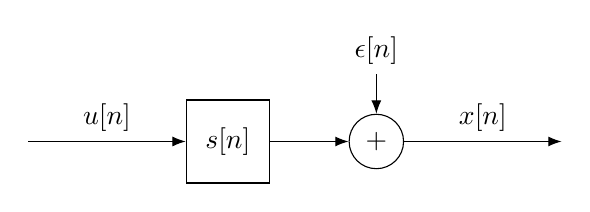
\begin{tikzpicture}[auto, node distance=2cm,>=Latex]
    % Nodos
    \node [input, name=input] {};
    \node [block, right=of input] (filter) {\(s[n]\)};
    \node [sum, right=of filter] (sum) {\(+\)};
    \node [output, right=of sum] (output) {};
    \node [above=0.5cm of sum] (noise) {\(\epsilon[n]\)};
    % Flechas
    \draw [->] (input) -- node {\(u[n]\)} (filter);
    \draw [->] (filter) -- node {} (sum);
    \draw [->] (sum) -- node [name=x] {\(x[n]\)} (output);
    \draw [->] (noise) -- node {} (sum);
\end{tikzpicture}
\caption{The signal model used in this chapter.}
\label{fig:linear_filter}
\end{figure}

For simplicity, we will assume that the input signal starts at $n=0$, that is, $u[n]=0$ for $n<0$. Also, we will assume that it is known; thus, a satistical model for $u[n]$ is unnecessary for our analysis).

The filtering problem consists in estimating the filter $s[n]$ from the input signal and a finite set of $N$ samples from the output, $x[0],\ldots, x[N-1]$. Also, we will tackle the output prediction problem: predicting unobserved values of the output for a given input signal $u[n]$.

Our goal is to solve the filtering problem using the tools from estimation theory developed in Chapter \ref{Estimation Theory}. To do so, we will first represent the target variables (the filter coefficients) and the observations (the output signal) in vector form, and the relation between them using a vector equation. Thus, we will join the nonzero coefficients in an $M$-dimensional vector
\begin{align}
\s &= \begin{bmatrix}
		s[0] \\ s[1] \\ \vdots \\ s[M-1]
      \end{bmatrix}_{M\times 1}.
\end{align}
Also, we will represent any $M$-length window of consecutive input values in vector form as
\begin{align}
\uu[n] &= \begin{bmatrix}
   	    	  u[n] \\ u[n-1] \\ \vdots \\ u[n-M+1]
          \end{bmatrix}_{M\times 1},
\end{align}
we can write
\begin{equation}
\label{eq:signal_model}
x[n] = \uu[n]^\top \s + \varepsilon[n].
\end{equation}

Note that, for any $n$, $\uu[n]$ contains only the input values that are relevant to compute $x[n]$.
% The filtering problem consists in estimating the filter coefficients $\s$ from a set of observed inputs and outputs, as well as estimating the output $x_*$ corresponding to a new input $\uu_*$.

Taking $n=0,1,\ldots,N-1$ in Eq. \eqref{eq:signal_model}, we get a system of $N$ linear equations relating the filter coefficients and the observations. We can join all of them into a single matrix equation by defining the observation vector
\begin{align}
\label{f:defx}
\x &= \begin{bmatrix}
                 x[0] \\ x[1] \\ \vdots \\ x[N-1]
      \end{bmatrix}_{N\times 1},
\end{align}
the input matrix
\begin{align}
\label{f:defU}
\UU &= [\uu[0]~~\uu[1]~\ldots~\uu[M-1]~\ldots~\uu[N-1] ]   \nonumber\\
    &= \begin{bmatrix}
                u[0]  & u[1]   & \ldots & u[M-1] & \ldots & u[N-1] \\
                0     & u[0]   & \ldots & u[M-2] & \ldots & u[N-2] \\
               \vdots & \vdots & \ddots & \vdots & \ldots & \vdots \\
               0      & 0      & \ldots & u[0]   & \ldots & u[N-M] 
       \end{bmatrix}_{M\times N},
\end{align}
and the noise vector
\begin{align}
\label{f:defeps}
\pmb{\epsilon} &= \begin{bmatrix}
                  \varepsilon[0] \\ \varepsilon[1] \\ \vdots \\ \varepsilon[N-1]
                  \end{bmatrix}_{N\times 1},
\end{align}
Using \eqref{f:defx}, \eqref{f:defU} \eqref{f:defeps}, we can write the signal model \eqref{eq:signal_model} as
\begin{framed}
\begin{equation}
\label{eq:signal_model_vec}
\x =\UU^\top \s + \pmb{\epsilon}
\end{equation}
\end{framed}

The filtering problem reduces to the problem of estimating $\s$ given $\x$ knowing \eqref{eq:signal_model_vec} and the noise statistics.

% Versión traspuesta, otra opción razonable de hacer las cosas...
%\begin{equation}
%\UU = 
%\left[ \begin{array}{l}
%\uu[0]  \\
%\uu[1]  \\
%\uu[M-1]  \\
%\vdots  \\
%\uu[N-1]  \\
%\end{array} \right]
%=
%\left[ \begin{array}{llll}
%u[0] & 0 & \ldots & 0 \\
%u[1] & u[0] & \ldots & 0 \\
%u[M-1] & u[M-2] & \ldots & u[0] \\
%\vdots & \vdots & \ddots & \vdots \\
%u[N-1] & u[N-2] & \ldots& u[N-M] \\
%\end{array} \right]
%\end{equation}


%%%%%%%%%%%%%%%%%%%%%
\section{ML solution}
%%%%%%%%%%%%%%%%%%%%%

Eq. \eqref{eq:signal_model} shows that, given $\s$, $x[n]$ is Gaussian with mean
\begin{align}
\EE\{x[n] \mid \s \} = \uu[n]^\top \s + \EE\{\varepsilon[n]\} = \uu[n]^\top \s 
\end{align}
and variance
\begin{align}
\EE\{(x[n]-\uu[n]^\top \s)^2 \mid\s \} = \sigma_\varepsilon^2 
\end{align}
that is, the likelihood function is
\begin{equation}
p(x[n] \mid \s ) = \Normal(x[n] \mid \uu[n]^\top\s, \sigma_\varepsilon^2),
\end{equation}
where the notation $\Normal(x \mid \mu, v) $ is used to refer to the \emph{normal} (Gaussian) pdf of a random variable with mean $\mu$ and variance $v$, evaluated at $x$.

Given $\s$, $x[n]$ depends on $\epsilon[n]$ only, which is an IID process. Thus, all samples from $x[n]$ are independent given $\s$, that is,
\begin{equation}
p_{{\bf X}|{\bf S}}(\x \mid \s) = \prod_{n=0}^{N-1} \Normal(x[n] \mid \uu[n]^\top\s, \sigma_\varepsilon^2) 
           = \Normal(\x \mid \UU^\top\s, \sigma_\varepsilon^2\eye).
\end{equation}

The value of $\s$ that maximizes $p(\x | \s)$ is
\begin{align}
\hat\s_\text{ML} 
   &= \argmax_{\s} p_{{\bf X}|{\bf S}}( \x \mid \s ) 
    = \argmax_{\s} \log p_{{\bf X}|{\bf S}}( \x \mid \s ) \nonumber \\
   &= \argmin_{\s} \frac{1}{2} (\x - \UU^\top\s)^\top(\sigma_\varepsilon^2\eye)^{-1}
                              (\x - \UU^\top\s) 
                + \frac{1}{2} \log|\sigma_\varepsilon^2\eye|+\frac{N}{2}\log(2\pi) 
                \nonumber \\
   &= \argmin_{\s} ||\x - \UU^\top\s||^2     \nonumber \\
\label{sml_comp}
\end{align}

This minimum can be easily obtained by taking the gradient with respect to $\s$, equalizing to zero and clearing, leading to
\begin{framed}
\begin{align}
\hat\s_\text{ML} &= (\UU \UU^\top)^{-1} \UU\x.
\label{sml}
\end{align}
\end{framed}

%%%%%%%%%%%%%%%%%%%%%%%%%%%
\section{Bayesian Solution}
%%%%%%%%%%%%%%%%%%%%%%%%%%%

To obtain a Bayesian estimator of $\s$ it is necessary to know its prior probability distribution, $p(\s)$. A common choice for this distribution is
\begin{equation}
p_{\bf S}(\s) = \Normal(\s | \mathbf{0}, \sigma_s^2\eye),
\end{equation}
since it accommodates any set of real coefficients and assumes they have a zero mean and a dispersion determined by $\sigma_s^2 $. It is also possible to set $\sigma_s^2 \rightarrow \infty$ to approach a uniform distribution. In any case, the use of this prior distribution enables the analytic derivation of the posterior distribution.

Given the likelihood, $p(\x | \s)$, and the prior distribution $p(\s)$, the posterior distribution $p(\s | \x) $ can be obtained. While it is feasible to directly apply Bayes' theorem and simplify the expression as much as possible, this process can be quite tedious. Instead, we will achieve the result in two steps.

First we will determine the joint pdf of $\s$ and $\x$. A simple way to do this is to observe that
\begin{equation}
\begin{bmatrix} \s \\ \x \end{bmatrix} =
	\begin{bmatrix} \eye  \\ \UU^\top          \end{bmatrix} \s + 
	\begin{bmatrix} \bf 0 \\ \pmb{\varepsilon} \end{bmatrix}
\end{equation}
%
that is, vector $[\s^\top~\x^\top]^\top$ is a linear combination of two Gaussian random vectors and, thus, is jointly Gaussian:
\begin{equation}
p_{{\bf S},{\bf X}}(\s,\x) 
	= \Normal\left(\begin{bmatrix} \s \\ \x \end{bmatrix}
                    \, \left| \,	                
	                \begin{bmatrix} {\bf m_S} \\ {\bf m_X} \end{bmatrix},
                    \begin{bmatrix} {\bf V_S}             & {\bf V_{SX}}   \\ 
                                    {\bf V}_{\bf SX}^\top & {\bf V_{X}}   
                    \end{bmatrix}
                    \right.
                    \right)
\end{equation}
where
\begin{align}
{\bf m_S}    &= \EE\{\s\} = {\bf 0}    \\
{\bf m_X}    &= \EE\{\x\} = {\bf U}^\top \EE\{\s\} + \EE\{\pmb{\epsilon}\} = {\bf 0}  \\
{\bf V_S}    &= \text{Var}\{\s\} = \sigma_s^2\eye     \\
{\bf V_{SX}} &= \EE\{\s\x^\top\} = \EE\{\s\s^\top\} \UU + \EE\{\s\pmb{\epsilon}^\top\}  = \sigma_s^2\UU \\
{\bf V_X} &= \EE\{\x\x^\top\} = \UU^\top \EE\{\s\s^\top\} \UU + \EE\{\pmb{\epsilon}\pmb{\epsilon}^\top\}  
           = \sigma_s^2\UU^\top\UU + \sigma_\varepsilon^2 \eye
\end{align}
Therefore,
\begin{align}
p_{{\bf S},{\bf X}}(\s,\x) 
	&= \Normal\left(
	      \begin{bmatrix} \s \\ \x \end{bmatrix}
          \, \left| \,	                
	      \begin{bmatrix} {\bf 0} \\ {\bf 0} \end{bmatrix},
          \begin{bmatrix} \sigma_s^2\eye     & \sigma_s^2\UU \\ 
                          \sigma_s^2\UU^\top & \sigma_s^2\UU^\top\UU + 
                                               \sigma_\varepsilon^2 \eye
          \end{bmatrix}
          \right.
          \right)
\label{eq:jointsx}
\end{align}
From previous chapter, we know that if $p_{{\bf S},{\bf X}}(\s,\x) $ is Gaussian, the conditional distribution $p_{{\bf S}|{\bf X}}(\s \mid \x) $ is also Gaussian, with mean and covariance
\begin{align}
\label{Filt:msx}
{\bf m}_{{\bf S}|{\bf X}} 
      &= {\bf m}_{\bf S} + {\bf V}_{\bf SX}{\bf V_X}^{-1}({\bf x}-{\bf m}_{\bf X})    \nonumber \\
      &= \UU \left(\UU^\top\UU + \tfrac{\sigma_\varepsilon^2}{\sigma_s^2} \eye \right)^{-1}\x \\
\label{Filt:vsx}
{\bf V}_{{\bf S}|{\bf X}} 
      &= {\bf V_S}- {\bf V}_{\bf SX}{\bf V_X}^{-1}{\bf V}_{\bf SX}^\top                \nonumber\\
      &= \sigma_s^2\eye 
       - \sigma_s^2\UU 
         \left(\UU^\top \UU + \tfrac{\sigma_\varepsilon^2}{\sigma_s^2}\eye\right)^{-1} \UU^\top   
\end{align}
The above expressions involve the computation of the inverse of an $N\times N$ matrix, which may be not feasible for large signal records (the computational cost is $\bigO (N^3)$. However, using the {\em matrix inversion lemma} (see the Appendix in Sec. \ref{Sec:mil}), we can obtain the following alternative expressions:
\begin{framed}\begin{align}
\label{Filt:sMMSEgaussMN2}
{\bf m}_{{\bf S}|{\bf X}} &= \PP \UU \x         \\
{\bf V}_{{\bf S}|{\bf X}} &= \sigma_\varepsilon^2 \PP   
\end{align}\end{framed}
where
\begin{framed}
\begin{equation}
\label{Filt:Pdef}
\PP = (\UU\UU^\top  + \tfrac{\sigma_\varepsilon^2}{\sigma_s^2}\eye)^{-1}.
\end{equation}
\end{framed}

Eq. \eqref{Filt:Pdef} involves the inversion of a matrix $M \times M$, which is usually much smaller than $N\times N$. 

Using these expressions, the MMSE, MAP and MAD estimates of $\s$ are:
\begin{framed}
\begin{equation}
\hat\s_\text{MSE} =\hat\s_\text{MAP} =\hat\s_\text{MAD} = \PP  \UU \x
\label{smmse}
\end{equation}
\end{framed}

Also, note that taking $\sigma_\varepsilon^2\rightarrow 0$ (negligible noise) and/or $\sigma_s^2\rightarrow\infty$ (which can be interpreted as assuming an infinitely wide uniform prior) these Bayesian solutions become equivalent to the ML in \eqref{sml}.


%%%%%%%%%%%%%%%%%%%%%%%%%%%%%%%%%%%%%%%%%%%%%%%%%%%%%%%%%%
\subsection{Probabilistic prediction of the filter output}

Once we have resolved several estimators of filter $\s$, we now begin to consider the problem of predicting a new output $x[k]$ at some time $k>N$. Continuing with the Bayesian perspective, we will obtain the posterior pdf of the target variable, $x[k]$, in light of the outputs already observed, $\x$. That is, we aim to calculate $p (x[k] \mid \x)$.

First, it should be noted that $\x, x[k]$ and $\s$ are jointly Gaussian. This follows from Eq. \eqref{eq:jointsx}, which can be extended to any arbitrary number of outputs, including $x[k]$. This necessarily implies that $\x$ and $x[k]$ are jointly Gaussian (when marginalizing $\s$) and finally that $p(x[k] | \x) $ must be Gaussian. Given that
\begin{equation}
x[k] = \uu[k]^\top\s+\varepsilon[k]
\end{equation}
is a linear transformation of $\s$ with independent white noise, we can easily compute the posterior mean and variance, respectively, as follows:
\begin{align}
\EE\{x[k]\mid \x\} &= \uu[k]^\top\EE\{\s\mid \x\} + \EE\{\varepsilon[k] \mid\x\}
                    = \uu[k]^\top\hat\s_\text{MSE}   \\
\text{Var}\{x[k] \mid \x\} 
	&= \EE\left\{\left(\uu[k]^\top \left(\s-\hat\s_\text{MSE}\right) 
	             + \varepsilon[k] \right)^2 \mid\x \right\}   \nonumber\\
    &= \uu[k]^\top \EE\{\left(\s-\hat\s_\text{MSE}\right)\left(\s-\hat\s_\text{MSE}\right)^\top 
                        \mid \x\} \uu[k]
       + \EE\{\varepsilon[k]^2 \mid\x\}    \nonumber\\
    &= \uu[k]^\top {\bf V}_{{\bf S}|{\bf X}} \uu[k] + \sigma_\varepsilon^2   \nonumber\\
    &= \sigma_\varepsilon^2 \uu[k]^\top \PP \uu[k] + \sigma_\varepsilon^2
\end{align}

Therefore, the Bayesian prediction of the output is succinctly given by
%
%\begin{equation}
%p(x[k] \mid \x) = \Normal(x[k] \mid \uu[k]^\top\PP  \UU \x,~~
%                    \sigma_\varepsilon^2+\sigma_\varepsilon^2\uu[k]^\top\PP \uu[k])
%\end{equation}.
\begin{framed}
\begin{equation}
\hat{x}_{\text{MSE} }[k] = \hat{x}_{\text{MAP} }[k] 
                         = \hat{x}_{\text{MAD} }[k]
                         = \uu[k]^\top\hat\s_\text{MSE}.
\label{Filt:xpred}
\end{equation}
\end{framed}

Eq. \eqref{Filt:xpred} shows that the optimal prediction of the output at any time $k>N$ can be computed by passing the input signal $u[n]$ though the filter with the coefficients in the Bayesian estimation of $\s$ (see Fig. \ref{fig:linear_filter2}).

%%%%%%%%%%%%%%%%%%%
\begin{figure}[htb]  % "htb" shows the location preference: here, up, down
    \centering
    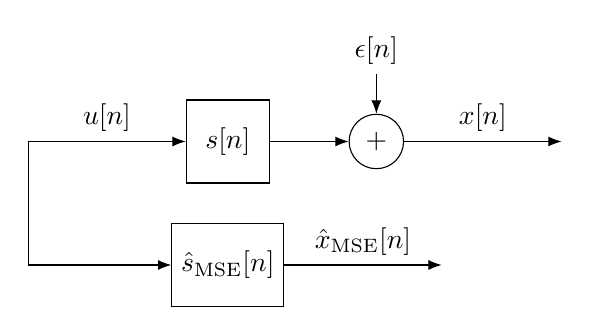
\begin{tikzpicture}[auto, node distance=2cm,>=Latex]
    % Nodos
    \node [input, name=input] {};
    \node [block, right=of input] (filter) {\(s[n]\)};
    \node [sum, right=of filter] (sum) {\(+\)};
    \node [output, right=of sum] (output) {};
    \node [above=0.5cm of sum] (noise) {\(\epsilon[n]\)};
    \node [block, below=0.5 cm of filter] (filterZ) {\(\hat{s}_\text{MSE}[n]\)}; % Nuevo filtro z[n]
    \node [output, right=of filterZ] (outputZ) {}; % Salida de z[n] como y'[n]

    % Flechas
    \draw [->] (input) -- node {\(u[n]\)} (filter);
    \draw [->] (filter) -- node {} (sum);
    \draw [->] (sum) -- node [name=y] {\(x[n]\)} (output);
    \draw [->] (noise) -- node {} (sum);
    \draw [->] (input) |- (filterZ); % Conexión de x[n] a z[n]
    \draw [->] (filterZ) -- node [name=yp] {\(\hat{x}_\text{MSE}[n]\)} (outputZ); % Salida de z[n] 
\end{tikzpicture}
\caption{The best prediction of future values of the output (knowing the input) can be computed by passing the input signal through a filter with the coefficients of the Bayesian estimation of $\s$.}
\label{fig:linear_filter2}
\end{figure}




% Para ello, calculamos
%\begin{align*}
%p(x_*|\x) &= \int_{\mathbb{R}^M} p(x_*, \s | \x) d\s ~~~~\text{      (marginalización de  $\s$)} \\
%&= \int_{\mathbb{R}^M} p(x_*|\s,\x) p(\s|\x) d\s~~~~\text{      (conjunta como producto de  condicional y marginal)} \\
%&= \int_{\mathbb{R}^M} p(x_*|\s) p(\s|\x) d\s~~~~\text{      (dado el filtro $\s$, las salidas son independientes entre sí)}. 
%\end{align*}

%%%%%%%%%%%%%%%%%%%%%%%%%
\section{Online calculus}
%%%%%%%%%%%%%%%%%%%%%%%%%

It is possible to obtain the above solutions online, that is, as new input-output pairs are obtained. While complete calculations could be repeated each time a new sample arrives, there are often more efficient ways to do this.

Note that estimating $\s$ using Eqs. \eqref{sml} or \eqref{smmse} requires inverting an $M \times M$ matrix. This has a cost $\bigO (M^3)$, that is, if we double the size of the filter, $M$ we multiply its computational cost by eight. Suppose now that you want to estimate $\s$ as new input-output pairs are received, that is, we are given first $\{u[0], x[0] \}$, then $\{u[1], x[1] \} $ and so on. In this case, we could reuse the results of the previous estimate to calculate the new updated estimate of $\s$, thus reducing the cost $\bigO(M^3) $ that would have a {\em naive} method that simply recalculates everything again every time a sample arrives.

%%%%%%%%%%%%%%%%%%%%%%%%%%%%%%
\subsection{Bayesian solution}

$\hat\s_\text{MSE}$ can be obtained exactly as more samples are available (i.e. as $N$ increases) without redoing all calculations, by reusing the previous solution. To do this, it is defined
\begin{align}
\PP_N &= (\UU \UU^\top + \tfrac{\sigma_\varepsilon^2}{\sigma_s^2}\eye)^{-1}, \\ \pp_N &= \UU \x
\end{align}
and the following recursive calculation is used (the first equation corresponds to the direct application of the matrix inversion lemma to the $\PP$ update):
\begin{align*}
\PP_{N+1} 
	&= \PP_N -\frac{\PP_N\uu[N+1]\uu[N+1]^\top 
	   \PP_N}{1  +\uu[N+1]^\top  \PP_N\uu[N+1]}  \\
\pp_{N+1} 
    &= \pp_N  +\uu[N+1] x[N+1] \\
\s_{N+1}
    &= \PP_{N+1}\pp_{N+1} ,
\end{align*}
which only has a cost $\bigO(M^2)$ per step (as opposed to applying the complete original equation at each step, which would cost $\bigO(M^3) $). This algorithm is called \emph{recursive least squares} (RLS).

%%%%%%%%%%%%%%%%%%%%%%%%
\subsection{ML solution}

An online approximation to $\hat\s_\text{ML}$ with computational cost $\bigO(M)$ can be obtained just by noting that
\begin{equation}
\hat\s_\text{ML} = \argmax_{\s} p(\x|\s) =  \argmin_{\s} ||\x - \UU^\top\s||^2
\end{equation}
and then use stochastic gradient to minimize $||\x - \UU^\top \s ||^2$.

Notice that
\begin{equation}
||\x - \UU^\top\s||^2 = \sum_{n=0}^{N-1} (x[n] - \uu[n]^\top\s)^2,
\end{equation}
so a gradient descent method would calculate the gradient of that expression and iteratively shift the estimate of the minimum in the opposite direction of the gradient in each step. A descent by stochastic gradient performs the same operation, but considering only one of the additions of the mentioned sum in each step. So,
the updating of coefficients that must be iterated to perform the minimization is in this case
\begin{equation}
\hat\s_{n+1} = \hat\s_n + \mu \left(x[n] - \uu[n]^\top \hat\s_n\right)\uu[n],
\end{equation}
where $\mu$ is an adaptation step that should be ``small enough''. This algorithm is called \emph{least mean squares} (LMS).

%%%%%%%%%%%%%%%%%%%%%%%%
%\section{Wiener filter}
%%%%%%%%%%%%%%%%%%%%%%%%
%
%The Wiener filter $\s_\text{Wiener}$ is the filter that minimizes the expected square error between a desired output $x[n]$ and the output produced when used to filter the input $u[n]$. In this section, both $x[n]$ and $u[n]$ are considered null half signals and $u[n]$ is treated as a stochastic process and not as a deterministic signal, as has been done up to now.
%
%This problem can be posed as a linear estimation problem of minimum mean square error (MMSE), so the formulation of the previous chapter can be used to give rise to the following solution:
%\begin{equation}
%\s_\text{Wiener} = \Ruu^{-1}\rux,
%\end{equation}
%where $\Ruu$ is the autocorrelation matrix of the input signal $u[n]$ and $\rux$ is the cross-correlation vector between $u[n]$ and $x[n]$. Unfortunately, these two quantities are generally unknown, so in most cases, the Wiener filter cannot be calculated. However, it is common to use the above expression using sample estimates for the correlation matrix $\hRuu = \tfrac{1}{N} \UU \UU^\top $ and the cross-correlation vector $\hrux = \tfrac{1}{N} \UU \x$. The result is an approximation to the Wiener filter $\hat\s_\text{Wiener} = \hRuu^{-1}\hrux$ that minimizes the sample quadratic error (often called ``least-squares estimate'') and which matches the ML solution, that is $\hat\s_\text{Wiener} = \hat \s_\text{ML}$.
%
%As the number of samples available for the estimation of the $\Ruu$ and $\rux$ statistics increases, these estimates become more precise, so that $\hat\s_\text {Wiener}$ and therefore $\hat\s_\text{ML}$ match asymptotically with the exact Wiener filter.


%%%%%%%%%%%%%%%%%%
\section{Problems}
%%%%%%%%%%%%%%%%%%

%%%%%%%%%%%%
\begin{prob}
\label{ProbFiltrado}

Consider the sequence
$$
u[1] \ldots u[7] \equiv 0.7,~-0.1,~0.7,~-0.2,~-0.1,~1.5,~-1.1
$$
which is fed as input to a linear filter of three coefficients, $\s = [s_1, s_2, s_3]^\top$. The following elements of the output sequence are known, (corrupted with Gaussian noise of variance 0.25):
$$
x[1] \ldots x[6] \equiv  -0.60,~1.13,~0.57,~0.42,~1.25,~-2.58
$$

\begin {itemize}
\item [a)] What is the ML estimate of $\s$ given the data? % (Wiener filter based on approximate statistics).
\item [b)] Use the obtained filter to predict $x[7]$, $\hat{x}_\text{ML}$.
\item [c)] Calculate the MSE, MAP and MAD estimates of $\s$ assuming that the prior pdf of its components is $s_i \sim \Normal(0,1)$ and that they are independent.
\item [d)] Get the MSE estimate of $x[7]$, $\hat{x}_\text{MSE}$.
\item [e)] Calculate the MSE in prediction b). (That is, the mean of $ (\hat{x}_\text{ML} -x[7])^2$ given the data).
\item [f)] Calculate the MSE in prediction d). (That is, the mean of $(\hat{x}_\text{MMSE} -x[6])^2 $ given the data)
\end{itemize}

\end{prob}
%%%%%%%%%%


%%%%%%%%%%%%%%%%%%%%%%%%%%%%%%%%%%%%%%%%%%%%%%%
\section{Appendix: the matrix inversion lemma}
\label{Sec:mil}

In this section we apply the matrix inversion lemma (also known as the Woodbury matrix identity) to obtain expression. This lemma states that, for any matrices ${\bf U}$, ${\bf C}$, ${bf V}$ and any non-singular matrix ${\bf A}$, 
\begin{align}
\left({\bf A} + {\bf V}{\bf C}{\bf U} \right)^{-1}
    = {\bf A}^{-1} 
    - {\bf A}^{-1}{\bf V} \left({\bf C}^{-1} 
    + {\bf U}{\bf A}^{-1}{\bf V} \right)^{-1} {\bf U}{\bf A}^{-1}
\end{align}
Proving this equality is not difficult: multiplying the right-hand side of the equality by ${\bf A} + {\bf U}{\bf C}{\bf V}$, it is easy to see that the result is the identity matrix.

Taking 
\begin{align}
{\bf A} &= \tfrac{\sigma_\varepsilon^2}{\sigma_s^2} \eye  \\
{\bf C} &= \eye      \\
{\bf V} &= \UU^\top
\end{align}
we get
\begin{align}
\label{Filt:mil}
\left(\UU^\top \UU + \tfrac{\sigma_\varepsilon^2}{\sigma_s^2}\eye \right)^{-1} 
    &= \tfrac{\sigma_s^2}{\sigma_\varepsilon^2}\eye 
	 - \left(\tfrac{\sigma_s^2}{\sigma_\varepsilon^2}\right)^2 \UU^\top 
	   \left(\eye + \tfrac{\sigma_s^2}{\sigma_\varepsilon^2} \UU \UU^\top \right)^{-1} 
	   \UU     \nonumber \\
    &= \tfrac{\sigma_s^2}{\sigma_\varepsilon^2}\eye 
	 - \tfrac{\sigma_s^2}{\sigma_\varepsilon^2} \UU^\top 
	   \left(\UU \UU^\top + \tfrac{\sigma_\varepsilon^2}{\sigma_s^2} \eye \right)^{-1} 
	   \UU   \nonumber\\
    &= \tfrac{\sigma_s^2}{\sigma_\varepsilon^2}\eye 
	 - \tfrac{\sigma_s^2}{\sigma_\varepsilon^2} \UU^\top 
	   \PP \UU
\end{align}
Where $\PP$ is given by \eqref{Filt:Pdef}. Note that, by definition,
\begin{align}
\left(\UU \UU^\top + \tfrac{\sigma_\varepsilon^2}{\sigma_s^2} \eye \right) \PP 
= \PP\left(\UU \UU^\top + \tfrac{\sigma_\varepsilon^2}{\sigma_s^2} \eye \right)  
= \eye 
\end{align}
so that
\begin{align}
\UU \UU^\top \PP = \PP \UU \UU^\top  = \eye - \tfrac{\sigma_\varepsilon^2}{\sigma_s^2} \PP
\end{align}
We will use these equalities below. Using \eqref{Filt:mil} into \eqref{Filt:msx}, we get
\begin{align}
\label{Filt:msx2}
{\bf m}_{{\bf S}|{\bf X}}
      &= \UU \left(\UU^\top\UU + \tfrac{\sigma_\varepsilon^2}{\sigma_s^2} \eye \right)^{-1}\x  
         \nonumber\\
      &= \tfrac{\sigma_s^2}{\sigma_\varepsilon^2} \UU \x 
    	   - \tfrac{\sigma_s^2}{\sigma_\varepsilon^2} 
    	     \UU \UU^\top  \PP 
	     \UU \x  \nonumber\\
      &= \tfrac{\sigma_s^2}{\sigma_\varepsilon^2} \UU \x 
    	   - \tfrac{\sigma_s^2}{\sigma_\varepsilon^2} 
    	     \left(\eye - \tfrac{\sigma_\varepsilon^2}{\sigma_s^2} \PP \right)
	     \UU \x  \nonumber\\
      &= \tfrac{\sigma_s^2}{\sigma_\varepsilon^2} \UU \x 
    	   - \tfrac{\sigma_s^2}{\sigma_\varepsilon^2} \UU \x 
    	   + \PP \UU \x  \nonumber\\
      &= \PP \UU \x  \\
{\bf V}_{{\bf S}|{\bf X}} 
      &= \sigma_s^2\eye 
       - \sigma_s^2\UU \left(\UU^\top \UU + \tfrac{\sigma_\varepsilon^2}{\sigma_s^2}\eye\right)^{-1}
          \UU^\top    \nonumber\\
      &= \sigma_s^2
         \left[  \eye 
               - \UU
                 \left(\tfrac{\sigma_s^2}{\sigma_\varepsilon^2}\eye 
     	             - \tfrac{\sigma_s^2}{\sigma_\varepsilon^2} \UU^\top\PP\UU
                 \right)
                 \UU^\top
         \right]    \nonumber\\
      &= \sigma_s^2
         \left[  \eye
               - \tfrac{\sigma_s^2}{\sigma_\varepsilon^2} \UU \UU^\top
               + \tfrac{\sigma_s^2}{\sigma_\varepsilon^2} \UU \UU^\top\PP\UU
                 \UU^\top
         \right]    \nonumber\\
      &= \sigma_s^2
         \left[  \eye
               - \tfrac{\sigma_s^2}{\sigma_\varepsilon^2} \UU \UU^\top
               + \tfrac{\sigma_s^2}{\sigma_\varepsilon^2} 
                 \left(\eye - \tfrac{\sigma_\varepsilon^2}{\sigma_s^2} \PP\right)\UU
                 \UU^\top
         \right]    \nonumber\\
      &= \sigma_\varepsilon^2 \PP
\end{align}



%%%%%%%%%%%%%%%%%%%%%%%%%%%%%%
% Chapter: Spectral estimation
\chapter{Spectral Estimation}
\mainmatter %%%%%%%%%%%%%%%%%%%%%%%%%%%%%%%%%%%%%%%%%%%%%%%%%%%%%%%
\tableofcontents
% \include{Contents/stochastic_processes/MC9_PSD_DRG}
\section{Introduction}

This chapter studies a very important estimation problem, which is that of estimating the power spectral density (PSD) of a stationary process. We will consider two families of estimators: 1) classical (or non-parametric) and parametric estimators, which are based on a model for the PSD.

Computing the estimate of $S_x(e^{j \omega})$, which we will denote by $\hat{S}_x(e^{j \omega})$, from an arbitrarily large number of realizations of a stationary process (see Figure \ref{fig:realizations_stochastic_process}) would be a (relatively) easy task. Of course, this is an idealized scenario as we do not have access to all realizations and, even more, we also do not have access to all time samples of the same realization. Thus, the objective in this chapter is to compute $\hat{S}_x(e^{j \omega})$ from $N$ samples of a single realization of the process $x[n]$.

The spectral estimation problem is defined only for wide-sense stationary (WSS) processes for which the mean function is time-independent, that is, $\mu_x = \mu_x[n] = \mathbb{E}[x[n]]$, and the auto-correlation function depends only on the time difference, i.e., $r_{x}[m] = r_{x}[n,n-m] = \mathbb{E}[x[n] x^{\ast}[n-m]]$. For non-stationary processes, the usual practice is to apply the estimators to small windows, since on a local scale we can assume that non-stationary processes are WSS. For instance, this is typically done when analyzing speech signals, which are usually described using non-stationary processes. Moreover, since only one realization is available, the process must be ergodic such that expectations can be substituted by time averages.

\begin{figure}
    \begin{center}
	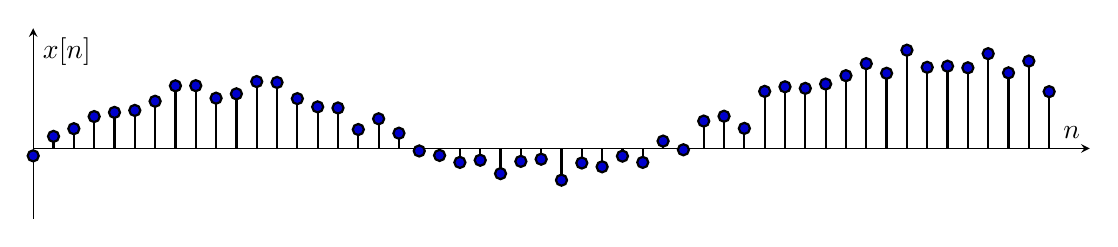
\begin{tikzpicture}
		\begin{axis}[%
		axis x line=middle,
		axis y line=middle,
		ticks=none,
		enlarge x limits=0,
		enlarge y limits=0.15,
		xmin=0,
		xmax=52,
		ymin=-1,
		width=15cm,
		height=4cm,
		domain = 0:50,
		samples = 51,
		xlabel={$n$},
		ylabel={$x[n]$}]
		\addplot+[ycomb,black,thick] {sin(2*180*x/35) + 0.3*rand + x/50 };
		\end{axis}
	\end{tikzpicture}
	\end{center}
    \begin{center}
	\huge{$\vdots$}
	\end{center}
	\begin{center}
	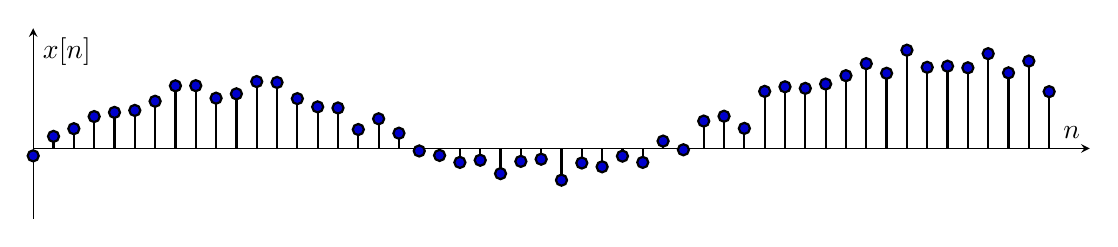
\begin{tikzpicture}
	\begin{axis}[%
		axis x line=middle,
		axis y line=middle,
		ticks=none,
		enlarge x limits=0,
		enlarge y limits=0.15,
		xmin=0,
		xmax=52,
		ymin=-1,
		width=15cm,
		height=4cm,
		domain = 0:50,
		samples = 51,
		xlabel={$n$},
		ylabel={$x[n]$}]
		\addplot+[ycomb,black,thick] {sin(2*180*x/35) + 0.3*rand + x/50};
\end{axis}
\end{tikzpicture}
	\end{center}
\caption{Realizations of a discrete stochastic process}
\label{fig:realizations_stochastic_process}
\end{figure}

\section{Preliminaries: Spectral analysis of deterministic signals}
\label{sec:preliminaries_deterministic_signals}
	
Before going into the spectral analysis of stochastic processes, it is convenient to study the case of deterministic signals, which will help us to understand the concept of spectral resolution. Thus, the problem is to compute the Fourier transform of the deterministic signal $x[n]$. However, this relatively ``simple'' task has two problems. First, we do not have access to the whole signal $x[n]$, but only to a finite record thereof
\begin{equation*}
   x_w[n]  = \begin{cases}
   x[n], & n = 0, \ldots, N-1, \\
   0, & \text{otherwise.}
   \end{cases}
\end{equation*}
Defining now the window
\begin{equation*}
w_{R,N}[n]  = \begin{cases}
1, & n = 0, \ldots, N-1, \\
0, & \text{otherwise,}
\end{cases}
\end{equation*}
we may rewrite $x_w[n] = w_{R,N}[n] x[n]$, which allows us to compute the Fourier transform of $x_w[n]$ as\footnote{In the ``Signals and Systems'' parlance, this Fourier transform is named Discrete Time Fourier Transform (DTFT).}
\begin{equation}
\label{eq:DTFT}
X_w(e^{j \omega}) = \mathcal{F} \left(x_w[n]\right) = \sum_{n = 0}^{N-1} x_w[n] e^{- j \omega N} = \frac{1}{2 \pi} W_{R,N}(e^{j \omega}) \circledast X(e^{j \omega}),
\end{equation}
where $\circledast$ denotes the circular convolution. So, the Fourier transform of the windowed signal, $x_w[n]$, is related to that of $x[n]$ through the Fourier transform of the window $w_{R,N}[n]$, which is given by
\begin{equation*}
W_{R,N}(e^{j \omega}) = e^{-j \omega (N-1)/2} \frac{\sin\left(\frac{\omega N}{2}\right)}{\sin\left(\frac{\omega}{2}\right)} = e^{-j \omega (N-1)/2} P_N(e^{j \omega}),
\end{equation*}
and its amplitude $|P_N(e^{j \omega})|$ is depicted in Figure \ref{fig:FT_rectangularwindow}. As this figure shows, the width of the main lobe is $4 \pi/N$.

\begin{figure}
	\pgfmathsetmacro{\mypi}{3.141592}
	\pgfmathsetmacro{\windowlength}{10}
	\begin{center}
		\begin{tikzpicture}
		\begin{axis}[%
		axis x line=middle,
		axis y line=middle,
		enlarge x limits=0.05,
		enlarge y limits=0.2,
		xtick={-\mypi,-2*\mypi/\windowlength,2*\mypi/\windowlength,\mypi},
		xticklabels={$-\pi$,$-\frac{2\pi}{N}$,$\frac{2\pi}{N}$,$\pi$},
		xmin=-\mypi,
		xmax=\mypi,
		ymin=0,
		ytick=\empty,
		width=10cm,
		height=7.5cm,
		domain = -\mypi:\mypi,
		samples = 512,
		xlabel={$\omega$},
		ylabel={$|P_N(e^{j \omega})|$}]
		%\addplot+[ycomb,black,thick] {x*\mypi};
		\addplot[black,thick] {abs(sin(deg(x*\windowlength/2))/sin(deg(x/2)))};
		\end{axis}
		\end{tikzpicture}
	\end{center}
	\caption{Module of the Fourier transform of the rectangular window}
	\label{fig:FT_rectangularwindow}
\end{figure}

The second issue is that the DTFT in \eqref{eq:DTFT} is a function of a continuous variable. Hence it cannot be computed nor stored in a computer. The solution is simple and consists in discretizing the spectrum, which yields the Discrete Fourier Transform (DFT). Thus, we are only able to compute $X_w(e^{j \omega_k}),$ with $\omega_k = 2 \pi k/N$ and $k = 0, \ldots, N-1$. The DFT is typically computed using the fast Fourier transform (FFT) algorithm. 

The aforementioned procedure based on the DFT/FFT gets only $N$ samples of the spectrum for length-$N$ signals, but we can get more samples by zero-padding the signals, i.e., by simply adding $N_\text{fft} - N$ zeros after the $N$ samples. This procedure increases the number of frequencies but it does not increase the resolution as it does not modify the window.
	
%%%%%%%%%%%%%%%
\begin{example}[Spectral analysis of a complex exponential]
	\label{ex:spectral_analysis_deterministic}
	
	This example considers the spectral analysis of a finite record of a complex exponential, i.e., $x[n] = e^{j \omega_0 n}, n = 0, \ldots, N-1$. Using the DTFT of a complex exponential, given by
\begin{equation*}
X(e^{j \omega}) = 2 \pi \delta(\omega - \omega_0),
\end{equation*}
and $W_N(e^{j \omega})$, $X_w(e^{j \omega})$ becomes
\begin{equation*}
X_w(e^{j \omega}) = e^{-j (\omega - \omega_0) (N-1)/2} \frac{\sin\left(\frac{(\omega - \omega_0) N}{2}\right)}{\sin\left(\frac{\omega - \omega_0}{2}\right)} =  e^{-j (\omega - \omega_0) (N-1)/2} P_N\left(\omega - \omega_0\right),
\end{equation*}
and its magnitude squared is
\begin{equation*}
|X_w(e^{j \omega})|^2 = \left|P_N\left(e^{j (\omega - \omega_0)}\right)\right|^2.
\end{equation*}
Figure \ref{fig:FT_complexexponential} plots, in logarithmic scale, $|X_w(e^{j \omega})|^2$ and $|X_w(e^{j \omega_k})|^2$ for two different values of $N_\text{fft}$.
\begin{figure}
	\pgfmathsetmacro{\mypi}{3.141592}
	\pgfmathsetmacro{\windowlength}{14}
	\pgfmathsetmacro{\myomega}{\mypi/8}
	\begin{center}
		\begin{tikzpicture}
		\begin{axis}[%
		axis x line=bottom,
		axis y line=middle,
		enlarge x limits=0.05,
		enlarge y limits=0.2,
		xtick={-\mypi,\myomega,\mypi},
		xticklabels={$-\pi$,$\omega_0$,$\pi$},
		xmin=-\mypi,
		xmax=\mypi,
		ymin=1e-3,
		ytick=\empty,
		ymode=log,
		width=8cm,
		height=6cm,
		domain = -\mypi:\mypi,
		samples = 512,
		xlabel={$\omega$},
		ylabel={$|X_w(e^{j \omega})|^2$}]
		%\addplot+[ycomb,black,thick] {x*\mypi};
		\addplot[black,thick] {(sin(deg((x-\myomega)*\windowlength/2))/sin(deg((x-\myomega)/2)))^2};
		\addplot+[only marks,mark=*,black,thick,each nth point=32] {(sin(deg((x-\myomega)*\windowlength/2))/sin(deg((x-\myomega)/2)))^2};
		\end{axis}
		\end{tikzpicture}
		\hspace{0.5cm}
		\begin{tikzpicture}
\begin{axis}[%
axis x line=bottom,
axis y line=middle,
enlarge x limits=0.05,
enlarge y limits=0.2,
xtick={-\mypi,\myomega,\mypi},
xticklabels={$-\pi$,$\omega_0$,$\pi$},
xmin=-\mypi,
xmax=\mypi,
ymin=1e-3,
ytick=\empty,
ymode=log,
width=8cm,
height=6cm,
domain = -\mypi:\mypi,
samples = 512,
xlabel={$\omega$},
ylabel={$|X_w(e^{j \omega})|^2$}]
\addplot[black,thick] {(sin(deg((x-\myomega)*\windowlength/2))/sin(deg((x-\myomega)/2)))^2};
\addplot+[only marks,mark=*,black,thick,each nth point=16] {(sin(deg((x-\myomega)*\windowlength/2))/sin(deg((x-\myomega)/2)))^2};
\end{axis}
\end{tikzpicture}
	\end{center}
	\caption{Fourier transform (in logarithmic scale) of a windowed complex exponential}
	\label{fig:FT_complexexponential}
\end{figure}
		
As we have seen in this example, the spectral analysis of deterministic signals depends on two factors. First, the number of available samples, which determines the window and, therefore, the shape of the windowed spectrum. As we have seen in Figure \ref{fig:FT_complexexponential}, the rectangular window has a narrow main lobe at the expense of high secondary lobes. This effect could be reduced by pre-multiplying $x_w[n]$ by a different window, which would reduce the height of the secondary lobes, but it would widen the main lobe.

\end{example}
%%%%%%%%%%%%%

%%%%%%%%%%%%%%%
\begin{example}[Spectral analysis of two complex exponentials]
	\label{ex:spectral_analysis_deterministic_two}
	
	This example considers the spectral analysis of a finite record of the sum of two complex exponential, i.e., $x[n] = e^{j \omega_0 n} + e^{j \omega_1 n}, n = 0, \ldots, N-1$, which will help us to understand the concept of resolution. Using \eqref{eq:DTFT}, we have
	\begin{equation*}
	X_w(e^{j \omega}) = e^{-j (\omega - \omega_0) (N-1)/2} P_N\left(\omega - \omega_0\right)+  e^{-j (\omega - \omega_1) (N-1)/2} P_N\left(\omega - \omega_1\right).
	\end{equation*}
	and its magnitude squared is
	\begin{multline*}
	|X_w(e^{j \omega})|^2 = \left|P_N\left(e^{j (\omega - \omega_0)}\right)\right|^2 + \left|P_N\left(e^{j (\omega - \omega_1)}\right)\right|^2  \\  + e^{j (\omega_0 - \omega_1) (N-1)/2} P_N\left(e^{j (\omega - \omega_0)}\right) P_N\left(e^{j (\omega - \omega_1)}\right)\\ +  e^{- j (\omega_0 - \omega_1) (N-1)/2} P_N\left(e^{j (\omega - \omega_0)}\right) P_N\left(e^{j (\omega - \omega_1)}\right).
\end{multline*}
Taking into account Euler's formula, $|X_w(e^{j \omega})|^2$ can be simplified as
	\begin{multline*}
|X_w(e^{j \omega})|^2 = \left|P_N\left(e^{j (\omega - \omega_0)}\right)\right|^2 + \left|P_N\left(e^{j (\omega - \omega_1)}\right)\right|^2  \\  + 2 \cos \left(\frac{(\omega_0 - \omega_1) (N-1)}{2} \right) P_N\left(e^{j (\omega - \omega_0)}\right) P_N\left(e^{j (\omega - \omega_1)}\right).
\end{multline*}
Figure \ref{fig:FT_twocomplexexponential} plots, in logarithmic scale, $|X_w(e^{j \omega})|^2$ for two different separations between the frequencies of the exponentials. As we can see in this figure, for small frequency separations, it is impossible to identify in the spectrum the two complex exponentials.
	\begin{figure}
		\pgfmathsetmacro{\mypi}{3.141592}
		\pgfmathsetmacro{\windowlength}{14}
		\pgfmathsetmacro{\myomega}{\mypi/8}
		\pgfmathsetmacro{\myomegabis}{3*\mypi/8}
		\pgfmathsetmacro{\myomegabisbis}{1.5*\mypi/8}
		\begin{center}
	\begin{tikzpicture}
\begin{axis}[%
axis x line=bottom,
axis y line=middle,
enlarge x limits=0.05,
enlarge y limits=0.2,
xtick={-\mypi,\myomega,\myomegabis,\mypi},
xticklabels={$-\pi$,$\omega_0$,$\omega_1$,$\pi$},
xmin=-\mypi,
xmax=\mypi,
ymin=1e-3,
ytick=\empty,
ymode=log,
width=8cm,
height=6cm,
domain = -\mypi:\mypi,
samples = 512,
xlabel={$\omega$},
ylabel={$|X_w(e^{j \omega})|^2$}]
\addplot[black,thick] {(sin(deg((x-\myomega)*\windowlength/2))/sin(deg((x-\myomega)/2)))^2 + (sin(deg((x-\myomegabis)*\windowlength/2))/sin(deg((x-\myomegabis)/2)))^2  + 2*cos(deg((\myomega - \myomegabis)*(\windowlength - 1)/2))*(sin(deg((x-\myomega)*\windowlength/2))/sin(deg((x-\myomega)/2)))*(sin(deg((x-\myomegabis)*\windowlength/2))/sin(deg((x-\myomegabis)/2)))};
\end{axis}
\end{tikzpicture}
	\begin{tikzpicture}
\begin{axis}[%
axis x line=bottom,
axis y line=middle,
enlarge x limits=0.05,
enlarge y limits=0.2,
xtick={-\mypi,\myomega,\mypi},
xticklabels={$-\pi$,$\omega_0$,$\pi$},
extra x ticks={\myomegabisbis},
extra x tick labels={$\omega_1$},
extra x tick style={tick label style={yshift=5mm}},
xmin=-\mypi,
xmax=\mypi,
ymin=1e-3,
ytick=\empty,
ymode=log,
width=8cm,
height=6cm,
domain = -\mypi:\mypi,
samples = 512,
xlabel={$\omega$},
ylabel={$|X_w(e^{j \omega})|^2$}]
\addplot[black,thick] {(sin(deg((x-\myomega)*\windowlength/2))/sin(deg((x-\myomega)/2)))^2 + (sin(deg((x-\myomegabisbis)*\windowlength/2))/sin(deg((x-\myomegabisbis)/2)))^2  + 2*cos(deg((\myomega - \myomegabisbis)*(\windowlength - 1)/2))*(sin(deg((x-\myomega)*\windowlength/2))/sin(deg((x-\myomega)/2)))*(sin(deg((x-\myomegabisbis)*\windowlength/2))/sin(deg((x-\myomegabisbis)/2)))};
\end{axis}
\end{tikzpicture}
		\end{center}
		\caption{Fourier transform (in logarithmic scale) of the sum of two complex exponentials}
		\label{fig:FT_twocomplexexponential}
	\end{figure}
	
\end{example}
%%%%%%%%%%%%%

\section{Non-parametric methods in spectral estimation}

In this section, we turn our attention to the case of stochastic signals and, in particular, to the development of non-parametric spectral estimation methods. We will therefore study the periodogram and variations thereof. 

Before proceeding, let us note that throughout this section, we will only consider DTFTs. However, we have to keep in mind that, in practice, we can only compute the DFT (using the FFT algorithm), as we have seen in Section \ref{sec:preliminaries_deterministic_signals}.

\subsection{The periodogram}

Despite the title section, we will start with an estimator known as correlogram, which is based on a first definition of the PSD.
\begin{definition}
	\label{wiener_khinchin}
	Given a WSS process $x[n]$, the power spectral density is defined as
	\begin{equation*}
	S_x(e^{j \omega}) = \mathcal{F}(r_{x}[m]),
	\end{equation*}
	where
	\begin{equation*}
	r_{x}[m] = \mathbb{E}[x[n] x^{\ast}[n-m]],
	\end{equation*}
	is the auto-correlation function of the process $x[n]$.
\end{definition}

Based on Definition \ref{wiener_khinchin}, the first estimator of the PSD is given by
\begin{equation*}
	\hat{S}_x(e^{j \omega}) = \mathcal{F}(\hat{r}_{x}[m]),
\end{equation*}
where $\hat{r}_{x}[m]$ is an estimator of the auto-correlation function. Concretely, we have two alternatives for this estimator: a biased and an unbiased estimator. The biased estimator of the auto-correlation, given the finite length $x[n], n = 0, \ldots, N-1$, is
\begin{equation}
	\label{eq:autocorrelation_biased}
	\hat{r}_{x}^{b}[m] = \frac{1}{N} \sum_{n = m}^{N-1} x[n] x^{\ast}[n-m], \quad m = 0, \ldots, N-1,
\end{equation}
and $\hat{r}_{x}^{b}[m] = \left[ \hat{r}_{x}^{b}[-m] \right]^{\ast}, m = -N+1, \ldots, -1$, whereas the unbiased estimator is
\begin{equation}
	\label{eq:autocorrelation_unbiased}
\hat{r}_{x}^{u}[m] = \frac{1}{N-m} \sum_{n = m}^{N-1} x[n] x^{\ast}[n-m], \quad m = 0, \ldots, N-1,
\end{equation}
and $\hat{r}_{x}^{u}[m] = \left[ \hat{r}_{x}^{u}[-m] \right]^{\ast}, m = -N+1, \ldots, -1$. Consequently, the PSD estimators are
\begin{equation}
\label{eq:correlogram}
\hat{S}_x^{b}(e^{j \omega}) = \mathcal{F}(\hat{r}_{x}^{b}[m]),
\end{equation}
and
\begin{equation*}
\hat{S}_x^{u}(e^{j \omega}) = \mathcal{F}(\hat{r}_{x}^{u}[m]).
\end{equation*}
Actually, only the estimator in \eqref{eq:correlogram}, which is known as the correlogram, is a valid PSD estimator since it ensures $\hat{S}_x^{b}(e^{j \omega}) \geq 0$, whereas $\hat{S}_x^{u}(e^{j \omega}) \not \geq 0$.

The periodogram, which is a term coined by Arthur Schuster in 1898, is based on a second definition of the power spectral density. This definition states that
\begin{equation*}
	S_x(e^{j \omega}) = \lim_{N \rightarrow \infty} \ E \left[\frac{1}{2N -1} \left| \sum_{n = -N+1}^{N-1} x[n] e^{-j \omega n} \right|^2 \right].
\end{equation*}
The periodogram is obtained from the above definition by simply dropping the expectation and considering a finite number of samples, i.e.,
\begin{equation}
	\label{eq:periodogram}
	\hat{S}_x^{p}(e^{j \omega}) = \frac{1}{N} \left| \sum_{n = 0}^{N-1} x[n] e^{-j \omega n} \right|^2 = \frac{1}{N} \left| X(e^{j \omega}) \right|^2,
\end{equation}
where $X(e^{j \omega})  = \mathcal{F}(x[n])$.

In the following, we will shed some light on why we have started this section with the correlogram. Let us start by rewriting $\hat{r}_{x}^{b}[m]$ as
\begin{equation*}
\hat{r}_{x}^{b}[m] = \frac{1}{N} \sum_{n = m}^{N-1} x[n] x^{\ast}[n-m] = \frac{1}{N} \sum_{n = -\infty}^{\infty} x[n] x^{\ast}[n-m]  = \frac{1}{N} \left(x[n] \ast x^{\ast}[-n]\right),
\end{equation*}
and taking its Fourier transform yields
\begin{equation*}
\hat{S}_x^{b}(e^{j \omega}) = \mathcal{F}(\hat{r}_{x}^{b}[m]) = \frac{1}{N} \mathcal{F} \left(x[n] \ast x^{\ast}[-n]\right).
\end{equation*}
Finally, applying the properties of the Fourier transform, $\hat{S}_x^{b}(e^{j \omega})$ simplifies to
\begin{equation*}
\hat{S}_x^{b}(e^{j \omega}) = \frac{1}{N} \mathcal{F} \left(x[n] \right) \mathcal{F} \left(x^{\ast}[-n]\right) = \frac{1}{N} X(e^{j \omega}) X^{\ast}(e^{j \omega}) = \frac{1}{N} \left| X(e^{j \omega}) \right|^2 = \hat{S}_x^{p}(e^{j \omega}),
\end{equation*}
which is the periodogram in \eqref{eq:periodogram}. That is, the periodogram and the correlogram are identical.

\subsubsection{Bias and variance of the periodogram}

To understand why we need more refined estimators of the power spectral density, now we shall perform the statistical analysis of the periodogram (or correlogram), i.e.,  we will compute its bias and variance as we would do with any other estimator.

The first question is whether the periodogram is a biased estimator of the PSD, that is, 
\begin{equation*}
E\left[\hat{S}_x^{p}(e^{j \omega}) \right] \mathop{=}^{?} S_x(e^{j \omega}).
\end{equation*}
To compute the bias of the periodogram, it is easier to consider the equivalence with the correlogram, which allows us to write
\begin{equation*}
E\left[\hat{S}_x^{p}(e^{j \omega}) \right] = E\left[\mathcal{F}(\hat{r}_{x}^{b}[m]) \right] = \mathcal{F}\left(E\left[ \hat{r}_{x}^{b}[m]\right]\right),  
\end{equation*}
where we have used that the expectation and the Fourier transform are both linear operators. Thus, the periodogram is biased if $\hat{r}_{x}^{b}[m]$ is a biased estimate of the auto-correlation function. Now, using the definition of  $\hat{r}_{x}^{b}[m]$, we get\footnote{It is easy to prove that $\hat{r}_{x}^{u}[m]$ is indeed an unbiased estimate of the auto-correlation function, which is left as an exercise for the student.}
\begin{multline*}
E\left[ \hat{r}_{x}^{b}[m]\right] = E\left[ \frac{1}{N} \sum_{n = m}^{N-1} x[n] x^{\ast}[n-m] \right] = \frac{1}{N} \sum_{n = m}^{N-1} E\left[ x[n] x^{\ast}[n-m] \right] \\ = \frac{1}{N} \sum_{n = m}^{N-1} r_{x}[m] = \frac{N - |m|}{N} r_{x}[m] \neq r_{x}[m],
\end{multline*}
which shows that $\hat{r}_{x}^{b}[m]$ is indeed a biased estimate of the auto-correlation function, with the exception of $m = 0$, and makes the periodogram a biased estimate of the PSD.

It is possible to obtain a closed-form expression for the bias of the periodogram by noting that
\begin{equation}
\label{eq:bias_auto-correlation}
E\left[\hat{r}_{x}^{b}[m]\right]  = \frac{N - |m|}{N} r_{x}[m] = w_{T,N}[m] r_{x}[m],
\end{equation}
where the triangular, or Barlett window, is defined as
\begin{equation*}
w_{T,N}[m] = \begin{cases} \frac{N - |m|}{N}, & |m| \leq N-1, \\
0, & \text{otherwise},
\end{cases}
\end{equation*}
and is depicted in Figure \ref{fig:triangularwindow}. The bias given in \eqref{eq:bias_auto-correlation} shows us that the larger the $m$ the larger the bias.
\begin{figure}
	\pgfmathsetmacro{\windowlength}{10}
	\begin{center}
		\begin{tikzpicture}
		\begin{axis}[%
		axis x line=middle,
		axis y line=middle,
		ticks=none,
		enlarge x limits=0.1,
		enlarge y limits=0.15,
		xmin=-\windowlength,
		xmax=\windowlength,
		ymin=0,
		ymax=1.2,
		width=10cm,
		height=7.5cm,
		domain = -\windowlength:\windowlength,
		samples = 2*\windowlength + 1,
		xlabel={$m$},
		ylabel={$w_{T,N}[m]$}]
		\addplot+[ycomb,black,thick] {(\windowlength - abs(x))/\windowlength};
		\end{axis}
		\end{tikzpicture}
	\end{center}
	\caption{Triangular window}
	\label{fig:triangularwindow}
\end{figure}


Using \eqref{eq:bias_auto-correlation}, the bias of the periodogram becomes
\begin{equation}
\label{eq:bias_periodogram}
E\left[\hat{S}_x^{p}(e^{j \omega}) \right] = \mathcal{F}\left(w_{T,N}[m] r_{x}[m]\right) = \frac{1}{2 \pi} W_{T,N}(e^{j \omega}) \circledast S_x(e^{j \omega}),
\end{equation}
where
\begin{align*}
W_{T,N}(e^{j \omega}) &= \mathcal{F}\left(w_{T,N}[m]\right) = \frac{1}{N} \mathcal{F}\left(w_{R,N}[m] \ast w_{R,N}[-m]\right) = |W_{R,N}(e^{j \omega})|^2 \nonumber  \\  &= \frac{1}{N} \frac{\sin^2\left(\frac{\omega N}{2}\right)}{\sin^2\left(\frac{\omega}{2}\right)},
\end{align*}
is the Fourier transform of the triangular window and is depicted in Figure \ref{fig:FT_triangularwindow}. Comparing Figures \ref{fig:FT_rectangularwindow} and \ref{fig:FT_triangularwindow}, it can be seen that the level of secondary lobes is smaller for the triangular window. By analogy with Example \ref{ex:spectral_analysis_deterministic_two}, we can say that the bias of the periodogram is related with its resolution.

\begin{figure}
	\pgfmathsetmacro{\mypi}{3.141592}
	\pgfmathsetmacro{\windowlength}{10}
	\begin{center}
		\begin{tikzpicture}
		\begin{axis}[%
		axis x line=middle,
		axis y line=middle,
		enlarge x limits=0.05,
		enlarge y limits=0.2,
		xtick={-\mypi,-2*\mypi/\windowlength,2*\mypi/\windowlength,\mypi},
		xticklabels={$-\pi$,$-\frac{2\pi}{N}$,$\frac{2\pi}{N}$,$\pi$},
		xmin=-\mypi,
		xmax=\mypi,
		ymin=0,
		ytick=\empty,
		width=10cm,
		height=7.5cm,
		domain = -\mypi:\mypi,
		samples = 512,
		xlabel={$\omega$},
		ylabel={$W_{T,N}(e^{j \omega})$}]
		\addplot[black,thick] {(sin(deg(x*\windowlength/2))/sin(deg(x/2)))^2};
		\end{axis}
		\end{tikzpicture}
	\end{center}
	\caption{Fourier transform of the triangular window}
	\label{fig:FT_triangularwindow}
\end{figure}

We have shown in \eqref{eq:bias_periodogram} that the periodogram is biased. However, there are some cases when it is not. For instance, considering the asymptotic regime, it is unbiased:
\begin{equation*}
\lim_{N \rightarrow \infty} \hat{S}_x^{p}(e^{j \omega}) = S_x(e^{j \omega}).
\end{equation*}
Another case is when the process $x[n]$ is white noise. For this kind of processes, $r_{x}[m] = \sigma^2_x \delta[m]$ and, therefore
\begin{equation*}
E\left[\hat{r}_{x}^{b}[m]\right]  = \frac{N - |m|}{N} r_{x}[m] = \sigma^2_x \delta[m] = r_{x}[m].
\end{equation*}
Since the estimate of the auto-correlation is unbiased for white processes, it is easy to show that the periodogram is also unbiased.

The analysis of the variance of the periodogram is cumbersome and can only be done in particular cases. For white noise, it can be shown that
\begin{equation*}
 \mathop{Var}\left(\hat{S}_x^{p}(e^{j \omega})\right) = S_x^{2}(e^{j \omega}),
\end{equation*}
and in general we can say that
\begin{equation*}
\mathop{Var}\left(\hat{S}_x^{p}(e^{j \omega})\right) \appropto S_x^{2}(e^{j \omega}),
\end{equation*}
where $\appropto$ denotes approximately proportional to.  This expression tells us that the variance does not decrease for larger data records. That is, the periodogram is not a consistent estimate of the PSD.

\subsection{The Blackman-Tukey estimator}

One of the reasons for the behavior of the periodogram variance is the poor quality of the estimate $\hat{r}_{x}^{b}[m]$ for values of $m$ close to $N$. This problem is what the Blackman-Tukey (BT) estimator tries to improve. The idea is to ignore or weight the samples of $\hat{r}_{x}^{b}[m]$ for $m$ close to $N$. Thus, the BT estimator is
\begin{equation}
\label{eq:BT_definition}
\hat{S}_x^{BT}(e^{j \omega}) = \mathcal{F}(w_M[m] \hat{r}_{x}^{b}[m]) = \sum_{m = -N + 1}^{N-1} w_M[m] \hat{r}_{x}^{b}[m] e^{-j \omega m},
\end{equation}
where $w[m]$ is a window that must fulfill
\begin{equation*}
w_{M}[m] = \begin{cases} f(|m|), & |m| \leq M-1, \\
0, & \text{otherwise},
\end{cases}
\end{equation*}
where $f(|m|)$ is a monotonically decreasing function of $|m|$ and $M \leq N$. This window ignores the lags of the estimated auto-correlation for $|m|>M-1$ and weights  the lags for large $m$. The choice of the window  is critical to achieve good performance, but, in any case, it must guarantee that $\hat{S}_x^{BT}(e^{j \omega}) \geq 0$.

Using the properties of the Fourier transform, we may rewrite $\hat{S}_x^{BT}(e^{j \omega})$ as
\begin{equation*}
\hat{S}_x^{BT}(e^{j \omega}) = \frac{1}{2 \pi} W_M(e^{j \omega}) \circledast \hat{S}_x^{p}(e^{j \omega}) = \frac{1}{2 \pi} \int_{-\pi}^{\pi} W_{M}(e^{j \psi}) \hat{S}_x^{p}(e^{j (\omega - \psi)}) d \psi,
\end{equation*} 
where $W_M(e^{j \omega}) = \mathcal{F}(w_M[n])$. Then, the Blackman-Tukey estimator is locally smoothing the periodogram, which reduces its variance. However, there is no free lunch and we will show that this variance reduction translates into lower resolution (or larger bias). Concretely, the bias of the BT estimator is
\begin{equation*}
E\left[\hat{S}_x^{BT}(e^{j \omega})\right] = \frac{1}{2 \pi} W_M(e^{j \omega}) \circledast E\left[\hat{S}_x^{p}(e^{j \omega})\right] = \frac{1}{2 \pi} W_M(e^{j \omega}) \circledast  W_{T,N}(e^{j \omega}) \circledast S_x(e^{j \omega}).
\end{equation*}
Finally, since $w_M[n]$ is shorter than $w_{T,N}[n]$, it can be shown that $W_M(e^{j \omega})$ is wider than $W_{T,M}(e^{j \omega})$, which translates into a lower resolution. This behavior is depicted in Figure \ref{fig:comparison_windows} for $w_M[n] = w_{T,M}[n]$. Note that the $y$-axis is in logarithmic scale.
\begin{figure}
	\pgfmathsetmacro{\mypi}{3.141592}
	\pgfmathsetmacro{\windowlength}{10}
	\pgfmathsetmacro{\windowlengthbis}{6}
	\begin{center}
		\begin{tikzpicture}
		\begin{axis}[%
		axis x line=bottom,
		axis y line=middle,
		enlarge x limits=0.05,
		enlarge y limits=0.2,
		xtick={-\mypi,-2*\mypi/\windowlengthbis,-2*\mypi/\windowlength,2*\mypi/\windowlength, 2*\mypi/\windowlengthbis,\mypi},
		xticklabels={$-\pi$,$-\frac{2\pi}{M}$,$-\frac{2\pi}{N}$,$\frac{2\pi}{N}$,$\frac{2\pi}{M}$,$\pi$},
		xmin=-\mypi,
		xmax=\mypi,
		ymin=1e-3,
		ymode=log,
		ytick=\empty,
		width=10cm,
		height=7.5cm,
		domain = -\mypi:\mypi,
		samples = 512,
		xlabel={$\omega$}]
		\addplot[black,thick] {(sin(deg(x*\windowlength/2))/sin(deg(x/2)))^2};
		\addplot[blue,thick] {2.8*(sin(deg(x*\windowlengthbis/2))/sin(deg(x/2)))^2};
		\legend{$W_{T,N}(e^{j \omega})$,$W_{T,M}(e^{j \omega})$};
		\end{axis}
		\end{tikzpicture}
	\end{center}
	\caption{Fourier transform (in logarithmic scale) of two triangular windows of different lengths}
	\label{fig:comparison_windows}
\end{figure}

\subsection{Estimators based on the averaged periodogram}

The Blackman-Tukey estimator yields a smaller variance than that of the periodogram because, as we have seen, it smooths the periodogram. An alternative to reduce the variance is to average several periodograms. However, the question is: How do we obtain such periodograms? The answer is easy and consists in dividing the $N$ observations into windows of length $M < N$. 

The Barlett method is one of the possible estimators based on the averaged periodogram. First, it divides the $N$ observations into $L$ non-overlapping windows of length $M$ as
\begin{equation*}
	x_l[n] = x[(l-1) M + n],
\end{equation*}
where $n = 0, \ldots, M-1,$ and $l = 1, \ldots, L$, and computes the periodogram of each window, that is,
\begin{equation*}
\hat{S}_{x,l}^{p}(e^{j \omega}) = \frac{1}{M} \left| \sum_{n = 0}^{M-1} x_l[n] e^{-j \omega n} \right|^2 = \frac{1}{M} \left| X_l(e^{j \omega}) \right|^2.
\end{equation*}
Then, the Barlett estimator is given by simply averaging the individual periodograms
\begin{equation*}
\hat{S}_{x}^{B}(e^{j \omega}) = \frac{1}{L} \sum_{l = 1}^{L}\hat{S}_{x,l}^{p}(e^{j \omega}).
\end{equation*}
Although it is out of the scope of these notes, we must point out that $\hat{S}_{x}^{B}(e^{j \omega})$ is somehow related to $\hat{S}_{x}^{BT}(e^{j \omega})$.

There are two further improvements of the periodogram. The first one is based on the Barlett estimator but substituting the individual periodograms by Blackman-Tukey estimates. The second one is based on dividing the $N$ observations into $L$ overlapping windows. The combination of both improvements is known as the Welch method.

One final question remains: What happens to the bias and variance of these methods. Regarding the bias (resolution), it is going to be smaller than that of the periodogram since $M < N$, as also happened to the Blackman-Tukey estimate. As for the variance, it is going to be reduced by a factor of $L$, the number of windows. That is,
\begin{equation*}
\mathop{Var}\left(\hat{S}_x^{ap}(e^{j \omega})\right) \approx \frac{1}{L} \mathop{Var}\left(\hat{S}_x^{p}(e^{j \omega})\right),
\end{equation*}
where $\hat{S}_x^{ap}(e^{j \omega})$ is any averaged periodogram (either Barlett or Welch methods) and $\approx$ is due to the non-independence between the windows. It would be an equality when the windows are independent, i.e., the Barlett method.

\section{Parametric methods in spectral estimation}

The problem of non-parametric methods is that they estimate an infinite number of parameters (the PSD at each frequency) from a sequence of $N$ observations. Clearly, this is an ill-posed problem since there are (many) more parameters to estimate than observations. To overcome this issue, we could postulate a parametric model for the PSD and estimate only the parameters of such model using the $N$ observations. For instance, the model could be $S_x(e^{j \omega})  = a + b \cos^2(\omega)$ and, hence, we only have to estimate $a$ and $b$.

Parametric approaches, as described above, can provide a significant performance boost if the signal fits the postulated model, otherwise the performance could be even worse than that of non-parametric methods. It is therefore of the utmost importance to select the proper model.

\subsection{Rational models for parametric spectral estimation}

These models consider a white Gaussian noise $u[n]$ with zero mean and variance $\sigma^2$ that goes through a causal and stable filter\footnote{A filter is said to be causal and stable if and only if all its poles are inside the unit circle.} $h[n]$ that has the following Fourier transform
\begin{equation*}
	H(e^{j \omega}) = \frac{B(e^{j \omega})}{A(e^{j \omega})} = \frac{\displaystyle \sum_{k = 0}^{q} b_k e^{-j \omega k}}{\displaystyle 1 + \sum_{k = 1}^{p} a_k e^{-j \omega k}},
\end{equation*}
which implies that
\begin{equation}
	\label{eq:signal_model_ARMA}
	x[n] = u[n] \ast h[n] = - \sum_{k = 1}^{p} a_k x[n -k] + \sum_{k = 0}^{q} b_k u[n-k].
\end{equation}
For these models, the PSD  is given by
\begin{equation}
\label{eq:PSD_ARMA}
S_x(e^{j \omega}) = S_u(e^{j \omega}) |H(e^{j \omega})|^2 = \sigma^2 \left|\frac{\displaystyle \sum_{k = 0}^{q} b_k e^{-j \omega k}}{\displaystyle 1 + \sum_{k = 1}^{p} a_k e^{-j \omega k}}\right|^2,
\end{equation}
and we only have to estimate $\sigma^2$, $a_1, \ldots, a_p$, and $b_0, \ldots, b_q$. 

According to Weierstrass theorem, for large values $p$ and $q$, the PSD model in \eqref{eq:PSD_ARMA} can approximate arbitrarily close any continuous PSD. Hence, there is a strong interest in this kind of models, which are named as auto-regressive moving average (ARMA or ARMA(p,q)). There are two special cases of the ARMA model that are particularly interesting: the auto-regressive (AR or AR(p)) and the moving average (MA or MA(q)). For the former, the PSD is given by
\begin{equation*}
S_x(e^{j \omega}) = \frac{\sigma^2}{\displaystyle \left|1 + \sum_{k = 1}^{p} a_k e^{-j \omega k}\right|^2},
\end{equation*}
whereas, for the latter, it is
\begin{equation*}
S_x(e^{j \omega}) =  \sigma^2 \left|\sum_{k = 0}^{q} b_k e^{-j \omega k}\right|^2.
\end{equation*}
AR models are good choices if we suspect the PSD has large peaks and MA models are good choices for PSDs with large valleys.

The estimation of the model parameters is typically carried out in the time domain, for which the auto-correlation structure is required. Once the auto-correlation function is available, which will depend in general on the model parameters in a non-linear fashion, the estimation procedure consists in substituting the theoretical auto-correlation by an estimate and then solving a non-linear system of equations. The PSD estimate is obtained by substituting the estimated parameters in the corresponding model. This procedure, which is conceptually simple, is actually rather involved. However, there is an exception, which is the AR model since the dependency of auto-correlation on the parameters is linear.

\subsection{The auto-correlation function of ARMA processes}

This section computes the auto-correlation function of ARMA processes, which is defined as
\begin{equation*}
	r_{x}[m] = \mathbb{E}[x[n] x^{\ast}[n-m]].
\end{equation*}
Substituting $x[n]$ by \eqref{eq:signal_model_ARMA}, $r_{x}[m]$ becomes
\begin{align*}
r_{x}[m] &= E\left[ \left(- \sum_{k = 1}^{p} a_k x[n -k]  + \sum_{k = 0}^{q} b_k u[n-k] \right) x^{\ast}[n-m]\right] \nonumber \\
&=  - \sum_{k = 1}^{p} a_k E\left[x[n -k] x^{\ast}[n-m]\right] + \sum_{k = 0}^{q} b_k  E\left[u[n-k]  x^{\ast}[n-m]\right] \nonumber \\
&=  - \sum_{k = 1}^{p} a_k r_{x}[m-k] + \sum_{k = 0}^{q} b_k  r_{ux}[m-k].
\end{align*}
where the cross-correlation function between $u[n]$ and $x[n]$ is
\begin{equation*}
r_{ux}[m] =   E\left[u[n]  x^{\ast}[n-m]\right].
\end{equation*}
Now, taking into account that
\begin{equation*}
x[n] = u[n] \ast h[n] = \sum_{l = -\infty}^{\infty} h[l] u[n-l],
\end{equation*}
the cross-correlation function becomes
\begin{align*}
r_{ux}[m] &=   E\left[u[n]  \sum_{l = -\infty}^{\infty} h^{\ast}[l] u^{\ast}[n-m-l]\right] \nonumber \\
&=   \sum_{l = -\infty}^{\infty} h^{\ast}[l] E\left[u[n]   u^{\ast}[n-m-l]\right] \nonumber \\
&=   \sum_{l = -\infty}^{\infty} h^{\ast}[l] r_u [m+l], \nonumber \\
&=   \sum_{l = -\infty}^{\infty} h^{\ast}[-l] r_u [m-l], \nonumber \\
&=   r_u [m] \ast h^{\ast}[-m],
\end{align*}
where the auto-correlation of $u[n]$ is
\begin{equation*}
r_{u}[m] = \mathbb{E}[u[n] u^{\ast}[n-m]] = \sigma^2 \delta[m],
\end{equation*}
because it is a white process. Then, $r_{ux}[m]$ simplifies to
\begin{equation*}
r_{ux}[m] =  \sigma^2 h^{\ast}[-m],
\end{equation*}
and plugging $r_{ux}[m]$ into $r_{x}[m]$, the desired auto-correlation becomes
\begin{equation*}
r_{x}[m] =  - \sum_{k = 1}^{p} a_k r_{x}[m-k] + \sigma^2 \sum_{k = 0}^{q} b_k  h^{\ast}[k-m].
\end{equation*}
The second term in the right-hand side of the the above equation can be expanded as
\begin{equation*}
\sigma^2 \sum_{k = 0}^{q} b_k  h^{\ast}[k-m] = \sigma^2  \left(b_0 h[-m] + b_1 h[1-m] + \ldots + b_q h[q-m]\right),
\end{equation*}
and since the filter is causal ($h[m] = 0, \forall m<0$), it becomes
\begin{align*}
\sigma^2  \sum_{k = 0}^{q} b_k  h^{\ast}[k-m] &= \begin{cases}
\sigma^2  \left(b_m h[0] + b_{m+1} h[1] + \ldots + b_q h[q-m]\right), & 0 \leq  m \leq q, \\ 
0, & m > q,
\end{cases} \nonumber \\
&= \begin{cases}
\displaystyle \sigma^2  \sum_{k = m}^{q} b_k  h^{\ast}[k-m], & 0 \leq  m \leq q, \\ 
0, & m > q.
\end{cases}
\end{align*}
Putting all pieces together we get
\begin{equation}
\label{eq:correlation_ARMA}
r_{x}[m] = \begin{cases}
\displaystyle - \sum_{k = 1}^{p} a_k r_{x}[m-k] + \sigma^2  \sum_{k = m}^{q} b_k  h^{\ast}[k-m], & 0 \leq  m \leq q, \\ 
\displaystyle  - \sum_{k = 1}^{p} a_k r_{x}[m-k], & m > q, \\
r_{x}^{\ast}[-m], & m < 0.
\end{cases}
\end{equation}
Keeping in mind that $h[m]$ will depend on $a_1, \ldots, a_p$, and $b_0, \ldots, b_q$, it is easy to see in \eqref{eq:correlation_ARMA} that the relationship between the model parameters ($\sigma^2$, $a_1, \ldots, a_p$, and $b_0, \ldots, b_q$) and the auto-correlation is non-linear, which complicates tremendously the estimation of such parameters from an estimate of the auto-correlation function. This is shown in the following example for a particular ARMA model.

\begin{example}[Auto-correlation function of an ARMA(1,1) process]
	
In this example, we will consider an ARMA(1,1) process, which has the following frequency response
\begin{equation*}
H(e^{j \omega}) = \frac{1 - b e^{-j \omega}}{1 - a e^{-j \omega}},
\end{equation*}
and the corresponding impulse response is
\begin{equation*}
h[n] = a^n s[n] - b a^{n-1} s[n-1],
\end{equation*}
where
\begin{equation*}
s[n] = \begin{cases}
1, & n \geq 0, \\
0, & n < 0.
\end{cases}
\end{equation*}
Now, we specialize \eqref{eq:correlation_ARMA} for the case of $p = 1, q = 1, b_0 = 1, b_1 = -b,$ and $a_1 = -a$, which yields
\begin{align*}
	r_x[0] &= a r_x[-1]  + \sigma^2 \left(1 + (-b) (a-b)^{\ast}\right), \\
	r_x[1] &= a r_x[0]  + \sigma^2  (-b), \\
	r_x[2] &= a r_x[1] , \\
	r_x[3] &= a r_x[2] , \\
	&\phantom{=} \vdots
\end{align*}
where we have taken into account that $h[0] = 1$ and $h[1] = a - b$. To recover the three model parameters, we need three equations, which are
\begin{equation*}
	\begin{bmatrix}
	r_x[0] & r_x[-1] \\
	r_x[1] & r_x[0] \\
	r_x[2] & r_x[1] 
	\end{bmatrix}
	\begin{bmatrix}
	1 \\ -a
	\end{bmatrix} = 
	\begin{bmatrix}
	\sigma^2 \left(1 - b (a-b)^{\ast}\right) \\
	\sigma^2  (-b) \\
	0
	\end{bmatrix}.
\end{equation*}
The first issue to solve the above system of equations is that we do not know $r_x[m]$, but as explained before it can be substituted by any estimator of the auto-correlation function, such as \eqref{eq:autocorrelation_biased} or \eqref{eq:autocorrelation_unbiased}, yielding
\begin{equation*}
	\begin{bmatrix}
	\hat{r}_x[0] & \hat{r}_x^{\ast}[1] \\
	\hat{r}_x[1] & \hat{r}_x[0] \\
	\hat{r}_x[2] & \hat{r}_x[1] 
\end{bmatrix}
\begin{bmatrix}
	1 \\ -a
\end{bmatrix} = 
\begin{bmatrix}
	\sigma^2 \left(1 - b (a-b)^{\ast}\right) \\
	\sigma^2  (-b) \\
	0
\end{bmatrix},
\end{equation*}
where we have used $\hat{r}_x[-1] = \hat{r}_x^{\ast}[1]$. The second issue is that the system of equations is non-linear, which makes it difficult to solve, even for this simple ARMA model.
\end{example}

\subsection{AR processes}

In the following, we will consider AR (= ARMA(p,0)) processes, which are the most commonly used ones among the three kind of processes studied in this course. There are several reasons. The first one is that the estimation of the parameters is much simpler. Actually, it can be done by simply solving a system of equations. Moreover, from the expression of an AR model
\begin{equation*}
x[n]  = u[n] - \sum_{k = 1}^{p} a_k x[n -k],
\end{equation*}
where we have assumed without loss of generality that $b_0 = 1$, we note that they can be used to predict future samples by ignoring the input, i.e.,
\begin{equation*}
x[n]  =  - \sum_{k = 1}^{p} \hat{a}_k x[n -k],
\end{equation*}
where the coefficient of the model have been replaced by some estimates. That is, from a record of $N$ samples, $x[0], \ldots, x[N-1]$, we can estimate the model parameters and, afterwards, we can predict $x[N], x[N+1], \ldots$

Let's now turn our attention to the estimation of the AR model parameters. Before proceeding, we shall require the impulse response of the system, which is given by
\begin{equation*}
h[n] = \left.x[n]\right|_{u[n] = \delta[n]} = \delta[n] - \sum_{k = 1}^{p} a_k h[n -k],
\end{equation*}
and since the filter is causal, we find that $h[0] = 1$, and allows us to particularize \eqref{eq:correlation_ARMA} as follows
\begin{equation}
\label{eq:correlation_AR}
r_{x}[m] = \begin{cases}
\displaystyle - \sum_{k = 1}^{p} a_k r_{x}[m-k] + \sigma^2  \overbrace{h^{\ast}[0]}^1, & m = 0, \\ 
\displaystyle  - \sum_{k = 1}^{p} a_k r_{x}[m-k], & m > 0, \\
r_{x}^{\ast}[-m], & m < 0.
\end{cases}
\end{equation}
Equation \eqref{eq:correlation_AR} shows that the auto-correlation function of the AR model does not depend on $h[n]$, which is the term that introduces non-linear relationships. Since we need to obtain $p+1$ parameters, i.e., $a_1, \ldots, a_p$ and $\sigma^2$, we need $p+1$ equations, which are
\begin{align*}
r_x[0] &= -a_1 r_x[-1] - a_2 r_x[-2] + \ldots -a_p r_x[-p] + \sigma^2, \\
r_x[1] &= -a_1 r_x[0] - a_2 r_x[-1] + \ldots -a_p r_x[-p+1], \\
r_x[2] &= -a_1 r_x[1] - a_2 r_x[0] + \ldots -a_p r_x[-p+2], \\
	&\phantom{=} \vdots \\
r_x[p] &= -a_1 r_x[p-1] - a_2 r_x[p-2] + \ldots -a_p r_x[0].
\end{align*}
The last $p$ equations depend only on $a_1, \ldots, a_p$. Writing them in matrix form, we get
\begin{equation*}
\begin{bmatrix}
r_x[0] & r_x[-1] & \cdots & r_x[-p+1] \\
r_x[1] & r_x[0] & \cdots & r_x[-p+2] \\
\vdots & \vdots & \ddots & \vdots \\
r_x[p-1] & r_x[p-2] & \cdots & r_x[0] 
\end{bmatrix}
\begin{bmatrix}
-a_1 \\ -a_2 \\ \vdots \\ -a_p
\end{bmatrix} = 
\begin{bmatrix}
r_x[1] \\ r_x[2] \\ \vdots \\ r_x[p]
\end{bmatrix},
\end{equation*}
which are known as the Yule-Walker equations. Hence, the filter coefficients are obtained by solving a linear system of equations
\begin{equation*}
\begin{bmatrix}
\hat{a}_1 \\ \hat{a}_2 \\ \vdots \\ \hat{a}_p
\end{bmatrix} = - \mathbf{R}_x^{-1} \mathbf{r}_x,
\end{equation*}
where 
\begin{equation*}
\mathbf{r}_x = \begin{bmatrix}
r_x[1] & r_x[2] & \cdots & r_x[p]
\end{bmatrix}^T,
\end{equation*}
and
\begin{equation*}
\mathbf{R}_x  =\begin{bmatrix}
r_x[0] & r_x^{\ast}[1] & \cdots & r_x^{\ast}[p-1] \\
r_x[1] & r_x[0] & \cdots & r_x^{\ast}[p-2] \\
\vdots & \vdots & \ddots & \vdots \\
r_x[p-1] & r_x[p-2] & \cdots & r_x[0] 
\end{bmatrix},
\end{equation*}
and we have used $r_{x}[-m] = r_{x}^{\ast}[m]$. The matrix $\mathbf{R}_x$ has a special structure, namely, it is constant along diagonals, and is therefore known as Toeplitz. This fact is important for solving the system of equations (computing the matrix inverse) as it reduces the complexity from $\mathcal{O}(p^3)$ to $\mathcal{O}(p^2)$. The remaining parameter to be estimated, the variance, is easily obtained as
\begin{equation*}
\hat{\sigma}^2 = r_x[0] + \hat{a}_1 r_x^{\ast}[1] + \hat{a}_2 r_x^{\ast}[2] + \ldots + \hat{a}_p r_x^{\ast}[p].
\end{equation*}
Finally, as we have already seen before, in practical scenarios the auto-correlation function is not available and must therefore be replace by an estimate.

\subsection{MA processes}

The last model considered in this course is MA (= ARMA(0,q)) processes, which have the following signal model
\begin{equation*}
x[n]  = \sum_{k = 0}^{q} b_k u[n-k].
\end{equation*}
In this case, the impulse response of the system is
\begin{equation*}
h[n] = b_n, \quad n = 0, \ldots, q,
\end{equation*}
and the auto-correlation in \eqref{eq:correlation_ARMA} becomes
\begin{equation*}
r_{x}[m] = \begin{cases}
\displaystyle \sigma^2  \sum_{k = m}^{q} h[k]  h^{\ast}[k-m], & 0 \leq  m \leq q, \\ 
0, & m > q, \\
r_{x}^{\ast}[-m], & m < 0.
\end{cases}
\end{equation*}
or, equivalently,
\begin{equation*}
r_{x}[m] = \begin{cases}
\displaystyle \sigma^2  h[m] \ast  h^{\ast}[-m], & 0 \leq  m \leq q, \\ 
0, & m > q, \\
r_{x}^{\ast}[-m], & m < 0.
\end{cases}
\end{equation*}
As in the ARMA model, the relationship between the auto-correlation function and the model parameters is non-linear, which is again shown in the following toy example.

\begin{example}[Auto-correlation function of a MA(1) process]
	
	In this example, we will consider a MA(1) process, which has the impulse response
	\begin{equation*}
	h[n] = h[0] \delta[n] + h[1] \delta[n-1].
	\end{equation*}
	For this $h[n]$, it is easy to find that
\begin{equation*}
h[m] \ast  h^{\ast}[-m] =
\begin{cases}
|h[0]|^2 + |h[1]|^2, & m = 0 \\
h^{\ast}[0] h[1], & m = 1 \\
h[0] h^{\ast}[1], & m = -1 \\
0, & |m| > 1.
\end{cases}
\end{equation*}
and the auto-correlation becomes
\begin{align*}
r_x[0] &= \sigma^2 \left(|h[0]|^2 + |h[1]|^2\right), \\
r_x[1] &= \sigma^2 h^{\ast}[0] h[1], \\
r_x[2] &= 0, \\
&\phantom{=} \vdots 
\end{align*}
Then, we have a non-linear system with $2$ equations and $3$ parameters, which cannot be solved. One could be tempted to add the equation corresponding to $r_x[-1]$ but it would not help as it is not independent. The actual solution is easier and is based on the fact that there is an amplitude ambiguity. That is, we will get the same output for $u[n]$ and $h[n]$ and for $u[n]/K$ and $K h[n]$. Thus, we can set one of the parameters to one, for instance, $h[0] = 1$, which yields
\begin{align*}
r_x[0] &= \sigma^2 \left(1 + |h[1]|^2\right), \\
r_x[1] &= \sigma^2 h[1].
\end{align*}
Dividing both equation we get
\begin{equation*}
\frac{r_x[0]}{r_x[1]} = \frac{1 + |h[1]|^2}{h[1]},
\end{equation*}
which is a second order polynomial and, as a consequence, there are two solutions for $h[1]$. Finally, for each of these solution, the estimate of the variance becomes
\begin{equation*}
\hat{\sigma}^2 = \frac{r_x[1]}{\hat{h}[1]}.
\end{equation*}

\end{example}

\backmatter%%%%%%%%%%%%%%%%%%%%%%%%%%%%%%%%%%%%%%%%%%%%%%%%%%%%%%%
%\include{Contents/glossary}
%\include{Contents/solutions}
\printindex
%%%%%%%%%%%%%%%%%%%%%%%%%%%%%%%%%%%%%%%%%%%%%%%%%%%%%%%%%%%%%%%%%%%%%%

\end{document}

%% Use the following syntax and markup for your references if 
%% the subject of your book is from the field 
%% "Computer Science, Economics, Engineering, Geosciences, Life Sciences"
%% Contribution 
%\bibitem{basic-contrib} Brown B, Aaron M (2001) The politics of nature. In: Smith J (ed) The rise of modern genomics, 3rd edn. Wiley, New York 
%% Online Document
%\bibitem{basic-online} Dod J (1999) Effective Substances. In: The dictionary of substances and their effects. Royal Society of Chemistry. Available via DIALOG. \\
%\url{http://www.rsc.org/dose/title of subordinate document. Cited 15 Jan 1999}
%% Journal article by DOI
%\bibitem{basic-DOI} Slifka MK, Whitton JL (2000) Clinical implications of dysregulated cytokine production. J Mol Med, doi: 10.1007/s001090000086
%% Journal article
%\bibitem{basic-journal} Smith J, Jones M Jr, Houghton L et al (1999) Future of health insurance. N Engl J Med 965:325--329
%% Monograph
%\bibitem{basic-mono} South J, Blass B (2001) The future of modern genomics. Blackwell, London 

\end{thebibliography}

\end{document}



























